\makeindex
%\documentclass[12 pt, oneside]{amsart}
%\documentclass[12 pt,oneside]{amsbook}
\documentclass[12 pt,oneside]{report}
%\documentclass[12 pt,oneside]{uvathesis}
\usepackage{epsfig}
\usepackage{amsmath}
\usepackage{rotating}
\usepackage{caption}
\usepackage{subfig}
\usepackage{graphicx}
\usepackage{booktabs}
\usepackage{epstopdf}
\usepackage{listings}
\usepackage{cite}
\usepackage{upquote}
\usepackage{xcolor}
\usepackage{pdfpages}
\usepackage[section]{placeins}

%This should be the last one
\usepackage{hyperref}
\usepackage{url} 
\usepackage{breakurl} 
%\documentclass[12 pt, oneside]{report}

\definecolor{dkgreen}{rgb}{0,0.6,0}
\definecolor{gray}{rgb}{0.5,0.5,0.5}
\definecolor{mauve}{rgb}{0.58,0,0.82}
\lstset{frame=tb,
  language=Java,
  aboveskip=3mm,
  belowskip=3mm,
  showstringspaces=false,
%  columns=flexible,
  basicstyle={\footnotesize\ttfamily},
  numbers=none,
  numberstyle=\tiny\color{gray},
  keywordstyle=\color{blue},
  commentstyle=\color{dkgreen},
  stringstyle=\color{mauve},
  breaklines=true,
  breakatwhitespace=true
  tabsize=1
}

\newcommand*{\TitleFont}{%
      \usefont{\encodingdefault}{\rmdefault}{b}{n}%
      \fontsize{16}{20}%
      \selectfont}

%%%%%%%%%%%%%%%%%%%%%%%%
%page shape
%%%%%%%%%%%%%%%%%%%%%%%%
%this file determines the shape of the page.

%%%%%%%%%%%%%%%%%%%%%%%%%%%%%%%%%%%%%%%%%

\usepackage{pagefix}
%changes size of page numbers
%to use this package 
%pagefix.sty must be in current dir.

%%%%%%%%%%%%%%%%%%%%%%%%%%%%%%%%%%%%%%%%%%%%%%
 
\setlength{\voffset}{3pt}
\setlength{\topmargin}{4pt}
\setlength{\headheight}{\baselineskip}
\setlength{\headsep}{25pt}
\setlength{\hoffset}{45pt}
\setlength{\oddsidemargin}{0pt}
\setlength{\marginparwidth}{0pt}
\setlength{\marginparpush}{0pt}
\setlength{\marginparsep}{0pt}
\setlength{\footskip}{14pt}
\setlength{\textwidth}{420pt}
\setlength{\textheight}{640pt}
 
%%%%%%%%%%%%%%%%%%%%%%%%%%%%%%%%%%%%%%%%%%%%%%%%%
%doublespacing:
\renewcommand{\baselinestretch}{1.5}

%%%%%%%%%%%%%%%%%%%%%%%%%%%%%%%%%%%%%%%%%%%%%%
 
%page numbers upper right corner:
%The oneside option must be used.

\pagestyle{plain}
%\markright{}

%%%%%%%%%%%%%%%%%%%%%%%%%%%%%%%%%%%%%%%%%%%%%%



\begin{document}

%%%%%%%%%%%%%%%%%%%%%%%%
% contents
%%%%%%%%%%%%%%%%%%%%%%%%
\input title.tex
\input abstract.tex
\input acknowledgement.tex

\tableofcontents
\listoffigures
\listoftables

%%%%%%%%%%%%%%%%%%%%%%%%%%%%%%%%%%%%%%%%%%%%%%%%%
%%%%%%%%%%%%introduction, prelim. %%%%%%%%%%%%%%%
%%%%%%%%%%%%%%%%%%%%%%%%%%%%%%%%%%%%%%%%%%%%%%%%%
%\setcounter{chapter}{1}
\input intro/intro.tex

%\setcounter{chapter}{2}
\input intro/src.tex

%\setcounter{chapter}{3}
\input setup/setup.tex

%\setcounter{chapter}{4}
\input analysis/analysis.tex

%\setcounter{chapter}{5}
\input cross_section/cross_section.tex

%\setcounter{chapter}{6}
\input cross_section/results.tex

%%%%%%%%%%%%% APPENDIX %%%%%%%%%%%%%%%%%%%%%%%%%%
\appendix
\chapter{Triggers in Data Analysis}
  This appendix is written specifically for people who analyze the Hall-A experiments or other experiments with similar trigger settings in Hall-A. It could also be useful for people who are interested in the event distributions in the trigger system and the trigger efficiency.
  
  When a scattered electron goes through the detectors located in the detector hut of each High Resolution Spectrometers (HRS), the signals created in specific detectors are used to form different triggers. The traditional single-arm production trigger, T1 for HRS-R or T3 for HRS-L, requires both the S1 and S2m scintillator planes to fire within a narrow time window. During the E08-014, a gas Cerenkov detector (GC) was also added into the production trigger in order to exclude most of pions events, and to reduce the total event rate as well as the dead-time. The new production triggers were the coincidence of logic signals from S1, S2m and GC. The original triggers were still used for the PID study but were assigned with different names, T6 for HRS-R and T7 for HRS-L, respectively. 

 Besides the main production triggers, there are two other important triggers, T2 for HRS-R and T4 for HRS-L, designed for the study of trigger efficiencies. Both T2 and T4 require only one of S1 and S2m logic signals to be coincident with the logic signal from a third detector plane, such as the GC in this experiment. The T2 and T4 triggers are generated by sending logic signals from S1, S2m and Cerenkov into a programmable module,called MLU~\cite{halla_daq}.

 Ideally, before the pre-scaling, T6 (T7) should be exactly the same as T1 (T3),if the GC has 100\% detection efficiency and there are no background events. However, T6 (T7) had much higher event rates than T1 (T3) mainly because of the pion contamination. During the data taking, the rates of  T1 and T3  were kept as high as possible until the dead time became high. T3, T4, T6 and T7 were prescaled to fix their rates no more than 50 $\sim$ 100Hz. T5, the coincident trigger of T1 and T3, was not used in this experiment and its rate was set to zero. T8 was the signal from the CPU clock and was also maintained at very low rate. 
\begin{table}[htbp]
 \begin{tabular}{lcccccccc}
 \toprule
 Trigger:       &    T1   &   T2   &   T3   &   T4   &   T5   &   T6   &   T7   &   T8\\
 \midrule
 TDC Channel:   &     1   &    2   &    3   &    4   &    5   &    6   &    7   &    8\\
 Decimal:       &     2   &   $\mathrm{2^{2}}$   &    $\mathrm{2^{3}}$   &   $\mathrm{2^{4}}$   &   $\mathrm{2^{5}}$   &  $\mathrm{2^{6}}$  &   $\mathrm{2^{7}}$  &   $\mathrm{2^{8}}$\\
 Hex:           &    0x02 &   0x04 &   0x08 &   0x10 &  0x20  &  0x40  &  0x80  &  0x100\\
 \bottomrule
 \end{tabular}
% \centering
\caption{Triggers and their corresponding data types in data stream}
\label{trigger_table}
\end{table}

 All these trigger signals are sent to a 16-channel TDC port. Signals produced by an event can generate several types of triggers in a very narrow time window. Once one of the triggers is accepted by the DAQ system, all of the event's signals from detectors and other instruments are recorded by TDCs and ADCs. The trigger signals associated with this event are also stored. The analyzer decodes the TDC values of these triggers in Hex format and issues these values into a pointer-like variable in the \emph{\bf{T}} tree, "DBB.evtypebits". Table~\ref{trigger_table} lists the triggers and their corresponding values in different digital types.

 Based on this table, events belonging to the same trigger can be identified by applying cuts on the trigger variable. Note that an event can be affiliated with more than one trigger types. There are several kinds of trigger cuts used during data analysis, where differences are listed below:
 \begin{enumerate}
\item \textbf{DBB.evtypebits=0x02}: \\
    Selecting events which are associated with T1 trigger only. The cut returns a value of "1".
\item \textbf{(DBB.evtypebits\&0x02)==0x02}: \\
    Selecting events which are associated with T1 trigger and may also be associated with other triggers. The cut returns a value of "1".
\item \textbf{DBB.evtypebits$\gg1$\&1}: \\
    The same as (2).
\item \textbf{DBB.evtypebits \&(1$\gg$1)}: \\
    Exactly the same as (2) and (3), but returning a value of "2" instead of "1" (all non-zero values mean "TRUE")

\emph{The following two trigger cuts are not recommended:}
\item \textbf{DBB.evtype==1}: \\
     Selecting events only triggered by T1, and not by any other triggers coming within 5~ms window when the TS registers an event.This is almost the same as (1) except a slight difference caused by unknown reasons. 
\item \textbf{fEvtHdr.fEvtType==1}:\\
     Exactly the same as (5)
\end{enumerate}
\begin{figure}[!ht]
 \begin{center}
  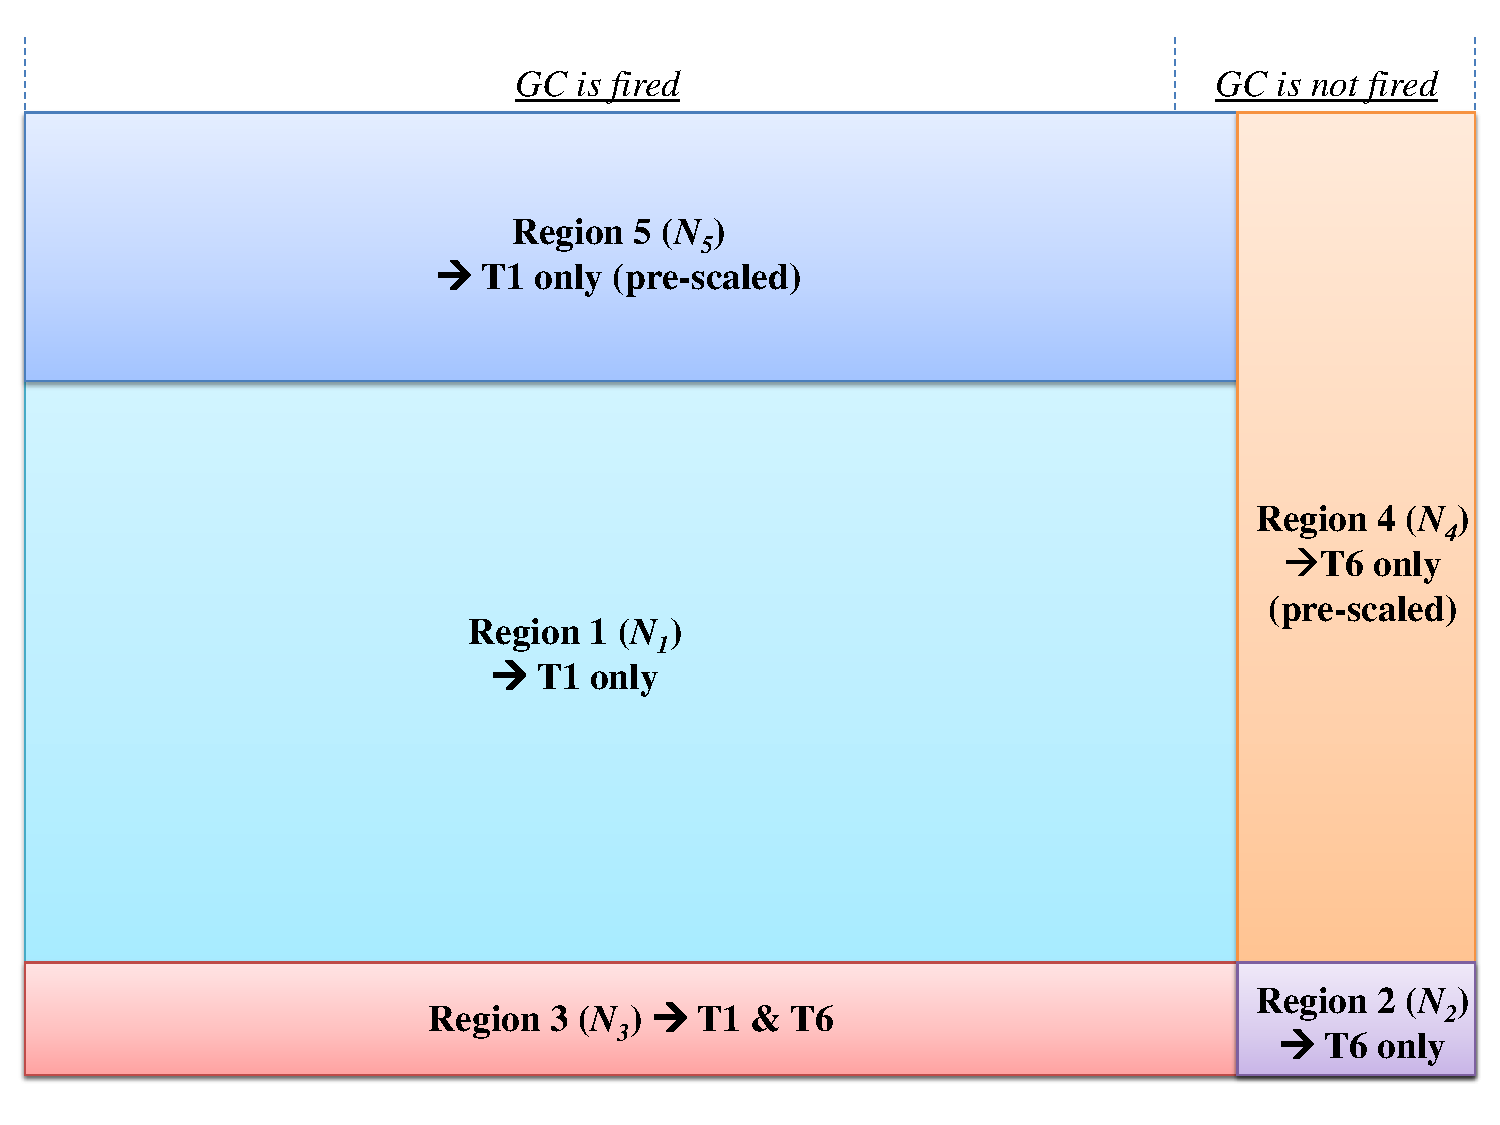
\includegraphics[width=0.6\textwidth]{./figures/trigger/trigger_region}
  \caption[A scheme of events with different trigger cuts]{A scheme of events with different trigger cuts. Each box denotes the number of events associated with certain trigger types. The size of each box does not necessarily reflect the real distribution of events in the data.}
  \label{trig_region}
 \end{center}
\end{figure}

  Not all the scattered electrons arriving in the detector hut can be recorded by the DAQ system because the detectors do not have 100\% detection efficiencies. Meanwhile, a certain portion of detected events are skipped as a result of pre-scaling. For each run, the pre-scale factors for different trigger types are recorded in the raw data as well as in the log files created at the start and at the end of each run. The total number of events from a trigger has to be corrected by the efficiency of the trigger system (i.e. the trigger efficiency) including the electronic, the computer and the detectors (S1, S2m and GC for E08014). The procedure to extract the trigger efficiency has been discussed in Section 5.5.1. In the rest of this section, all variables related to the number of events are assumed to have been corrected by the trigger efficiency.
   
  Assuming the total number of the scattered electrons which fire both S1 and S2m on HRS-R is given as the big box in Fig.~\ref{trig_region}, the area of each small box represents the number of electrons (events) associated with different trigger types after applying the pre-scale factors. Region 1 gives the number of events ($\mathrm{N_{1}}$) from T1 only, and region 2 gives the total number of event ($\mathrm{N_{2}}$) from T6 only. Region 3 represents the events associated with both T1 and T6 ($\mathrm{N_{3}}$). The portions of events which are not recorded due to the pre-scaling are given as $\mathrm{N_{4}}$ in Region 4 for T6 and $\mathrm{N_{5}}$ in Region 5 for T1, respectively. $\mathrm{N_{2}+ N_{4}}$ denotes the number of events which are not detected by the GC, and it should be small since the GC has a very high detection efficiency. So the relationship between the number of events in those regions and the pre-scale factors can given as:
 \begin{equation}
 PS1 = \frac{N_{1}+N_{3}+N_{5}}{N_{1}+N_{3}},  PS6 = \frac{N_{1}+N_{2}+N_{3}+N_{4}+N_{5}}{N_{2}+N_{3}}=\frac{N_{2}+N_{4}}{N_{2}},
\end{equation}
 where $\mathrm{N_{1}}$, $\mathrm{N_{2}}$ and $\mathrm{N_{3}}$ can be extracted from data by applying Trigger cuts as listed in Table~\ref{trigger_cut_table}.
\begin{table}[htbp]
 \begin{tabular}{lcc}
\toprule
 Events  &  Cut\\
\midrule
$N_{1}$  &  \textbf{DBB.evtypebits$\gg1\&1$\&\&!(DBB.evtypebits$\gg6\&1$)} \\
$N_{2}$  &  \textbf{DBB.evtypebits$\gg6\&1$\&\&!(DBB.evtypebits$\gg1\&1$)} \\
$N_{3}$  &  \textbf{DBB.evtypebits$\gg1\&1$\&\&DBB.evtypebits$\gg6\&1$}  \\
$N_{1}+N_{3}$  &  \textbf{DBB.evtypebits$\gg1\&1$}  \\
$N_{2}+N_{3}$  &  \textbf{DBB.evtypebits$\gg6\&1$}  \\
\bottomrule
  \end{tabular}
  \caption[Events types with different Trigger cuts]{Events types with different Trigger cuts}
  \label{trigger_cut_table}
\end{table}

 If the pre-scale factors are known, the total number of trigger events in the box can be mathematically calculated:
\begin{equation}
 N_{0} = N_{1}+N_{2}+N_{3}+N_{4}+N_{5}=PS6\times(N_{2}+N_{3}).
\end{equation}
However, since the pre-scale factor of T6 was set to be large enough to keep the trigger rate around 50Hz, the value of $N_{2}+N_{3}$ should be very small and the statistical error in $\mathrm{N_{0}}$ would be very large. However, $\mathrm{N_{1}}$ has much more statistics since T1 was maintained to have big trigger rate. Combined with $\mathrm{N_{4}}$ and $\mathrm{N_{5}}$, it gives the total number of electrons in that box as:
\begin{equation}
 N_{0} = N_{1}+N_{2}+N_{3}+N_{4}+N_{5}=PS1\times(N_{1}+N_{3})+PS6\times N_{2}.
\label{event0_1}
\end{equation}
where the term, $PS1\times(N_{1}+N_{3})$, denotes the number of events which fired the GC, while $PS6\times N_{2}$ is the number of electrons which did not fire the detector. 

\begin{figure}[!ht]
 \begin{center}
  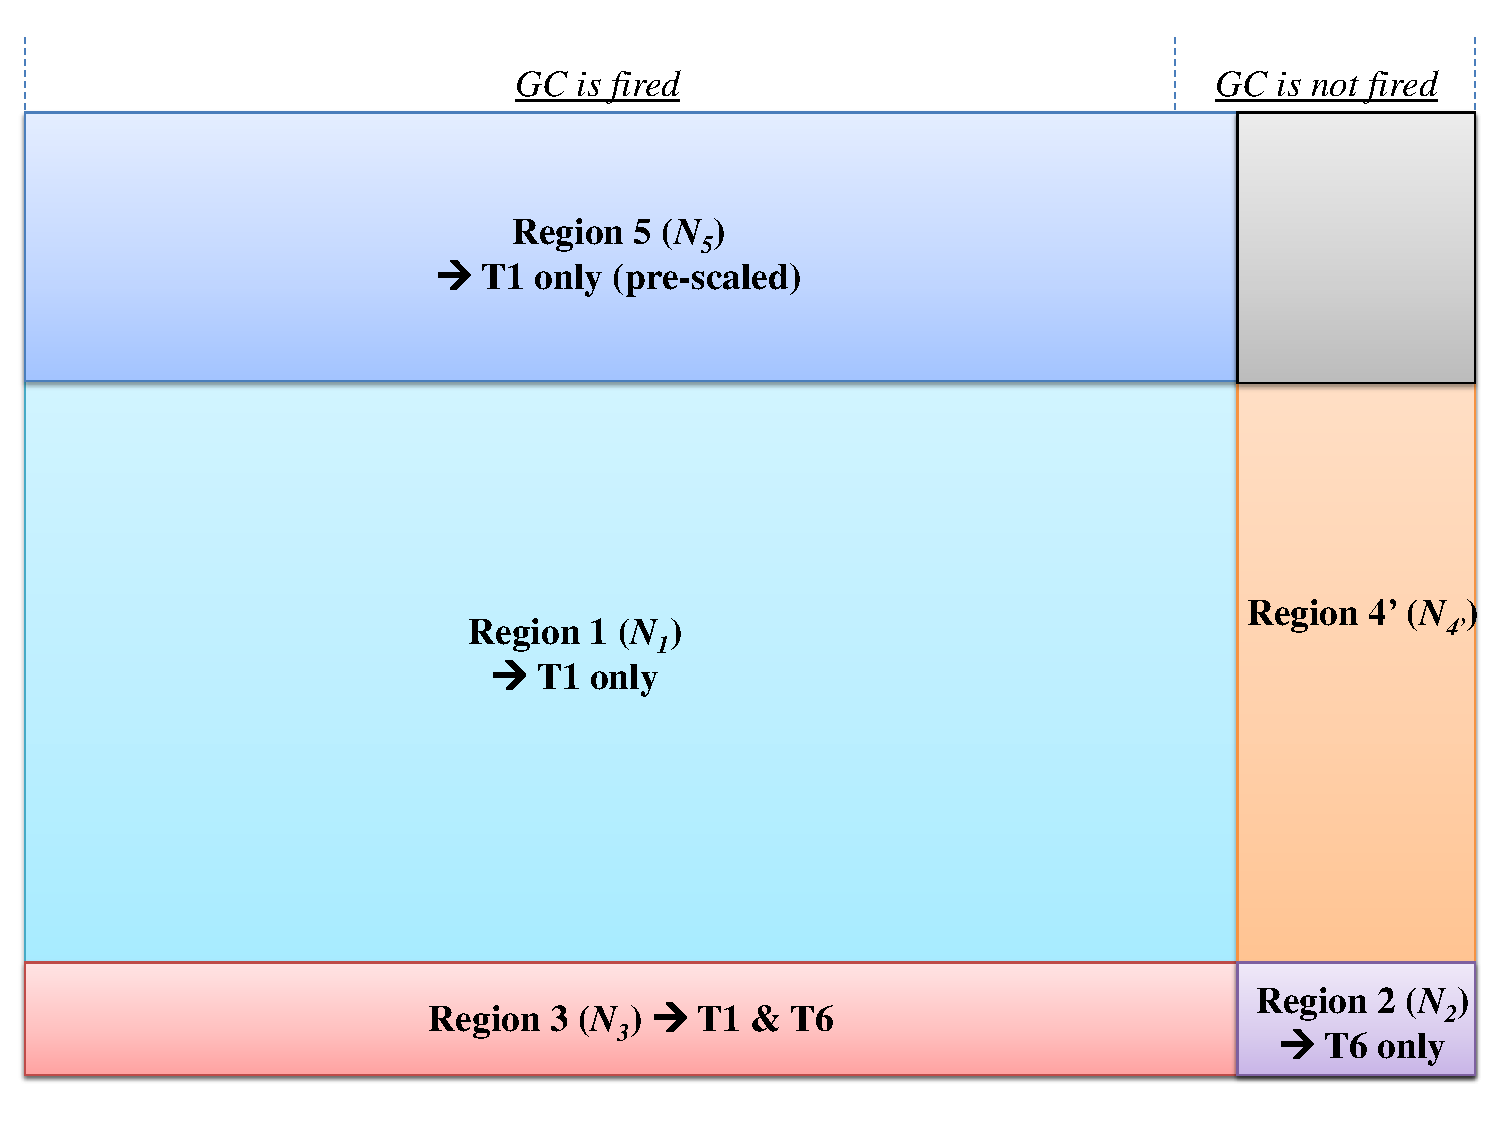
\includegraphics[width=0.6\textwidth]{./figures/trigger/trigger_region2}
  \caption[Another scheme of electrons with different trigger cuts]{Another scheme of electrons with different trigger cuts}
  \label{trig_region2}
 \end{center}
\end{figure}

Eq.~\ref{event0_1} can be further simplified. From Fig.~\ref{trig_region2}, a new region, called Region 4' ($N_{4'}$), can be defined:
\begin{equation}
\frac{N_{4'}}{N_{1}}=\frac{N_{2}}{N_{3}}=\frac{N_{2}+N_{4}}{N_{1}+N_{3}+N_{5}},
\end{equation}
which gives:
\begin{equation}
 N_{2}+N{4} = PS6\times N_{2} = PS1\times(N_{2}+N{4'}) = PS1\times(N_{2}+N_{1}N_{2}/N_{3}).
\end{equation}
and the relationship between PS1 and PS6 can be given by:
\begin{equation}
 PS6 = PS1(1+N_{1}/N_{3}).
\end{equation}

 So PS6 can be substituted by the formula above, and Eq.~\ref{event0_1} becomes:
\begin{equation}
 N_{0} = PS1\times(N_{1}+N_{3})\times \frac{N_{2}+N_{3}}{N_{3}}=\frac{PS1\times(N_{1}+N_{3})}{\epsilon},
\label{event0_2}
\end{equation}
where $\epsilon=\frac{N_{3}}{N_{2}+N_{3}}$ is the percentage of electrons firing GC when they pass through the detector, i.e. the exact definition of the GC detection efficiency. Since the number of events from T6 is very small, to reduce the statistical error, the typical way to get the detection efficiency of the GC is to select good electron samples from T1 events by applying a tight cut on the calorimeter and determining how many of them are detected by the GC (see Section 5.5.3): 
\begin{equation}
 \epsilon_{det}^{GC}=\frac{N^{GC}}{N^{Sample\_from\_Calo}}.
\end{equation}

 Based on the discussion above, $\mathrm{N_{0}}$ becomes straightforward: the total number of electrons passing through the HRS detectors is equal to the number of events triggered by S1, S2m and GC and corrected by the detection efficiency of the GC. It is important to emphasize that the value of $\mathrm{N_{0}}$ has to also be corrected by the trigger efficiency which is only related to the performance of S1 and S2m.
 
 The total number of trigger events from T3 on HRS-L can also be given in the same way.
\chapter{XEMC: A Package for Inclusive Cross Section Models}

\section{Overview}
 XEMC is a stand-alone package written in C++ to calculate the inclusive cross section of electron-nucleus scattering. It is composed of three cross section models for the inelastic (DIS) process, three cross section models for the quasi-elastic (QE) process, and a radiative correction (RC) subroutine based on the peak approximation. In this model, the Born cross section ($\mathrm{\sigma^{Born}_{model}}$) is the sum of the inelastic cross section ($\mathrm{\sigma^{DIS}_{model}}$) and the QE cross section ($\mathrm{\sigma^{QE}_{model}})$. The RC subroutine calculates the radiative cross section ($\mathrm{\sigma^{rad}_{model}}$) from the Born cross section. The parameters of kinematic settings and target configurations are all defined in an external file.
 
 Cross section models are usually developed based on theoretical calculations, world data and additional corrections. Different models are designed for specific kinematic regions, depending on the physics processes and the final states. The inclusive cross section measured by the E08-014 was above the QE peak and can be well modelled by the y-scaling~\cite{West1975263,PhysRevC.41.R2474,Boffi19931,john_thesis}. The QE model was further iterated through comparing with experimental data at the similar kinematics. The DIS contribution to the total cross section was small and was calculated with the most updated DIS model~\cite{Bosted:2012qc}. 
  
  The basic structure of the package will be briefly introduced here, followed by a discussion of the cross section models. The results calculated with this code will be compared with experiment results. And a simple example of how to use this code is also given in the end. 
  
\section{Code Structure}
\begin{figure}[!ht]
 \begin{center}
  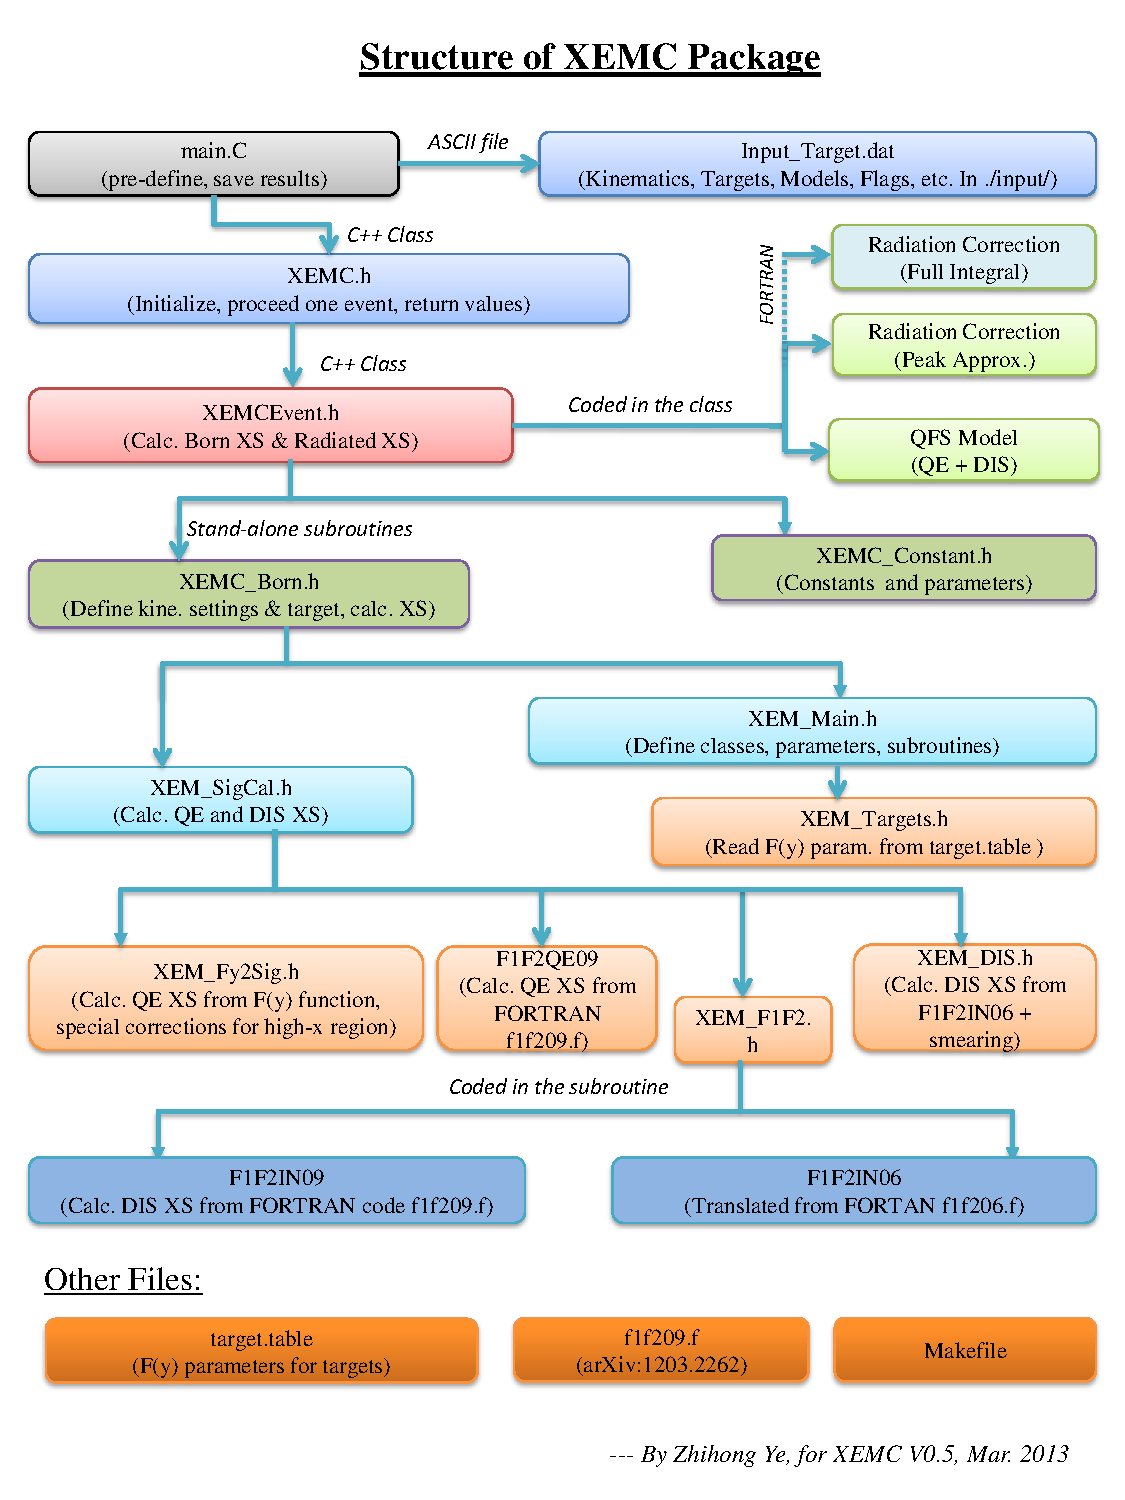
\includegraphics[angle=0,width=1.0\textwidth]{./figures/xemc/XEMC_Structure}
  \caption[Structure of XEMC package]{Structure of XEMC package}
  \label{xemc_struct}
 \end{center}
\end{figure}
\begin{figure}[!ht]
 \begin{center}
  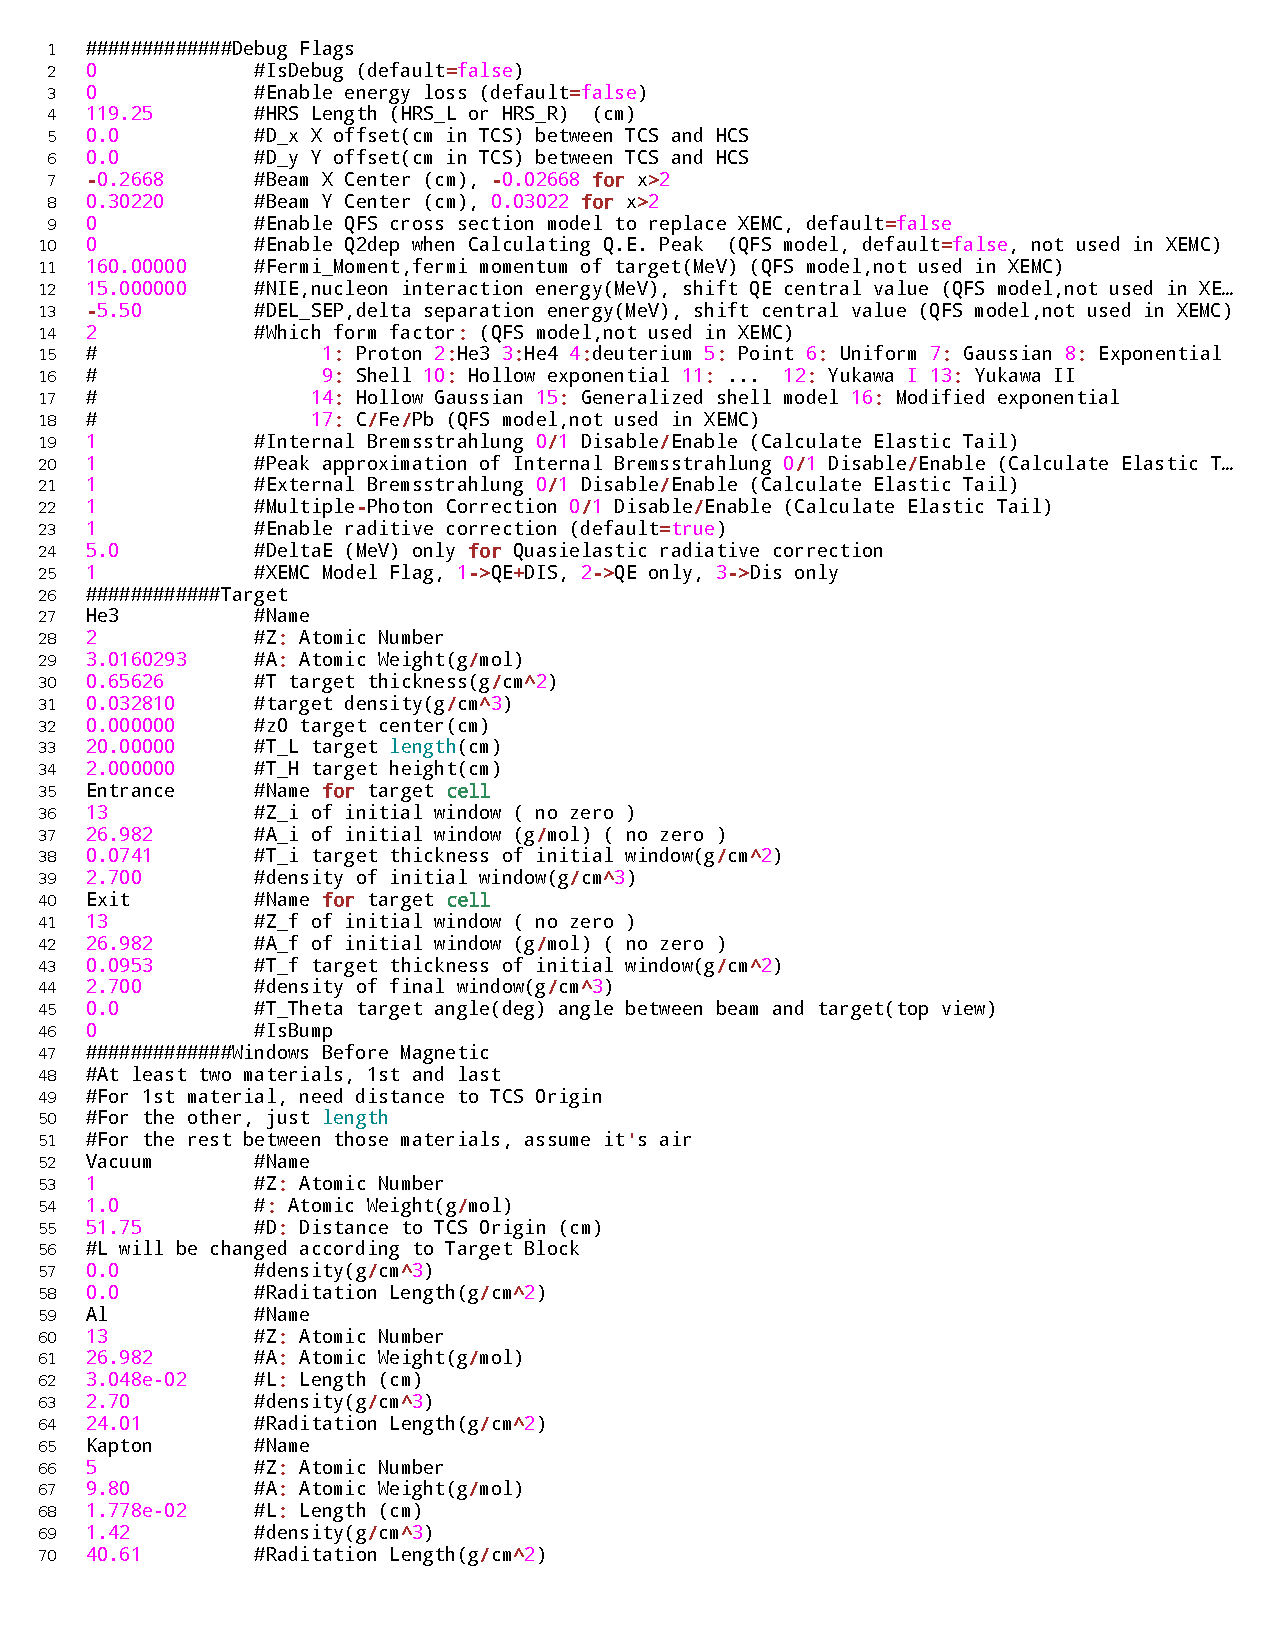
\includegraphics[angle=0,width=1.01\textwidth]{./figures/xemc/He3_Input}
 \caption[Input file for $\mathrm{^{3}He}$ target]{Input file for $\mathrm{^{3}He}$ target}
 \label{xemc_tgt_he3}
 \end{center}
\end{figure} 
Fig.~\ref{xemc_struct} shows the basic structure of the XEMC package. Outside the main code, the input file (Fig.~\ref{xemc_tgt_he3}) is defined to specify the choice of cross section models and any additional physics processes, such as the radiative correction. The reaction location can be corrected by giving the spectrometer center offset and beam position offset. The input file also includes the configuration of the target system, i.e. the target's name, mass and thickness. For cryo-targets, the materials of the target cell, the entrance and the exit of the target chamber are also given. Parameters in the input file are initialized only once in the code.

  A XEMC event has its specified values of the initial and scattered energies as well as the scattering angle. The Born cross section and radiated cross section of this event are calculated in \emph{XEMCEvent.h} where the QFS model is embedded by default.  Other Born cross section models are stored in an independent subroutine, \emph{$\mathrm{XEMC\_Born.h}$}, which will be introduced in next few sections. Once the target configuration and the kinematic setting are pre-defined, the RC subroutine in \emph{XEMCEvent.h} begins to calculate the radiated cross section. 

\section{Quasi-Elastic Cross Section Models}
 Three different QE cross section models, QE-XEM, QE-QFS, and QE-F1F209, are coded in this package. Each model will be introduced below.

 \subsection{QE-XEM} 
  \begin{figure}[!ht]
 \begin{center}
  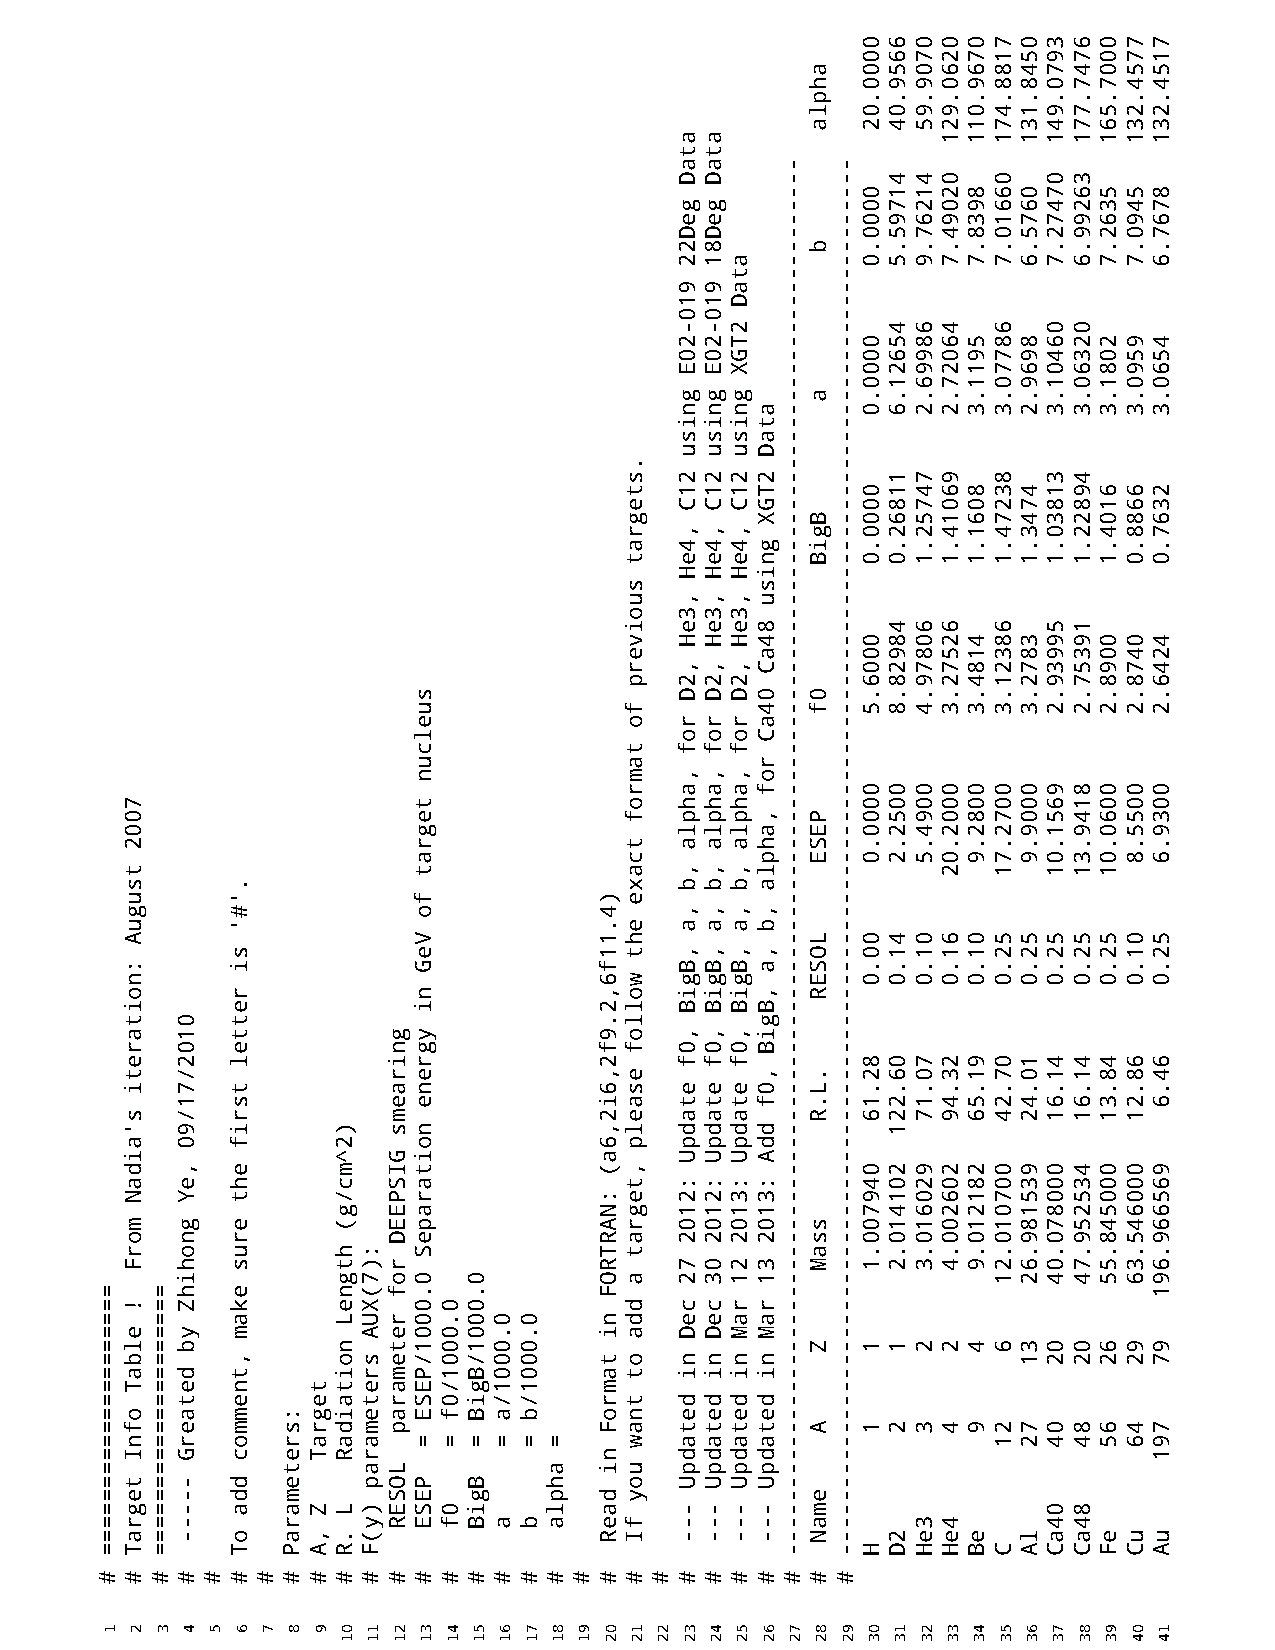
\includegraphics[angle=0,width=1.0\textwidth]{./figures/xemc/target_table}
  \caption[F(y) parameters for a list of targets]{F(y) parameters for a list of target. The file is called target.table which is in ASCII format. The values had been refitted with cross section results from the E02-019 and the E08-014. These values could be changed in the future.}
  \label{xemc_tgt_table}
 \end{center}
\end{figure} 

 QE-XEM was converted from the XEM cross section model, a FORTRAN package developed by the EMC collaboration in Hall-C at JLab~\cite{nadia_thesis,aji_thesis}. XEM includes a QE model (QE-XEM) based on y-scaling~\cite{West1975263,PhysRevC.41.R2474,Boffi19931,john_thesis}, a DIS model (DIS-XEM, see next section), and a RC subroutine. The entire subroutines have been converted into C++ (except the RC part) and coded in \emph{$XEMC\_Born.h$}. QE-XEM is the default QE model in the package.
 
  The scaling function, F(y) (Eq.~\eqref{fy_scaling_eq2} in Section 1.2.2), is directly fitted from experimental data. F(y) for $\mathrm{^{2}H}$ can be extracted from the function~\cite{PhysRevLett.56.1452}:
  \begin{equation}
  F(y) = (f_{0}-B)\frac{\alpha^{2}e^{-(\alpha y)^{2}}}{\alpha^{2}+y^{2}} + B e^{-b|y|},
  \label{fy_fit_func1}
  \end{equation}
where, $f_{0}$, $B$, $\alpha$, $a$ and $b$ are the parameters corresponding to the target. For heavy targets, the second term in the formula above is different:
  \begin{equation}
  F(y) = (f_{0}-B)\frac{\alpha^{2}e^{-(\alpha y)^{2}}}{\alpha^{2}+y^{2}} + B e^{-(by)^{2}}.
    \label{fy_fit_func2}
  \end{equation}

  For a list of targets, the parameters of $F(y)$ function ($f_{},~B,~\alpha,~a,~and~b$) are stored in an external ASCII file, called \emph{target.table}. To extract the parameters, one needs to  obtain the distribution of $F(y)$ from the experimental cross sections:
  \begin{equation}
   F(y) = \sigma_{EX}^{QE}\cdot\frac{1}{Z\sigma_{p}+N\sigma_{n}}\frac{q}{\sqrt{M^{2}+(y+q)^{2}}},
  \end{equation}
where $q=\sqrt{Q^{2}+\nu^{2}}$, and $y$ is the solution of the equation:
\begin{equation}
  M_{A}+\nu = \sqrt{M^{2}+q^{2}+y^{2}+2yq}+\sqrt{M_{A-1}^{2}+y^{2}},
\end{equation}
where $M$ is the mass of the struck nucleon, $M_{A}$ and $M_{A-1}$ are the masses of the target nucleus and the mass of the recoil system, respectively.

 The experimental QE cross sections, $\sigma_{EX}^{QE}$, can be extracted from the experimental Born cross sections subtracted by the DIS cross sections calculated from the model, i.e. $\sigma_{EX}^{QE}=\sigma_{EX}^{Born}-\sigma_{model}^{DIS}$. Hence, different DIS models yield different fitting values of the F(y) parameters. Fig.~\ref{xemc_tgt_table} gives a target table which lists the values of these parameters for all measured targets. The parameters have been determined from the the E02-019~\cite{nadia_thesis} and the E08-014 data with the DIS model, DIS-F1F209 (discussed in Section B.4.3). 
 
 \subsection{QE-QFS}
  QE-QFS is based on the QFS model, a phenomenological model~\cite{qfs_org,qfs_note} which has been used since 1960s. The model was designed to calculate both QE and DIS cross sections with the Plane-Wave Impulse Approximation (PWIA) and it works well at lower $Q^{2}$ region. The complete description of the QFS model can be found in Ref.~\cite{qfs_org,qfs_org2}. The subroutines of the model are coded in $XEMCEvent.h$ and were originally developed and maintained by the collaboration from Temple University~\cite{karl_thesis, hyao_thesis,whita}. 
   
 \subsection{QE-F1F209}
 QE-F1F209 is a part of the cross section model, F1F2QE09, which was developed by P. Bosted and V. Mamyan~\cite{Bosted:2012qc} based their work on empirical fit to electron-nucleus scattering. The model is coded in a stand-alone FORTRAN program, \emph{f1f209.f}. An external link is given in the XEMC package to call the subroutines in the FORTRAN code. To successfully compile the code, a library named \emph{libg2c.so} must be specified in the \emph{Makefile}.
 
\section{DIS Models}
 The DIS cross section model not only calculates the cross section of the deep inelastic scattering process but also includes other inelastic processes, such as resonance productions. There are three DIS models coded in the package. Since the kinematic settings of the E08-014 was well above the QE peak, the contribution from inelastic processes is relatively small, and these models were not iterated with the existing DIS data. 
 
\subsection{DIS-QFS}
 DIS-QFS is a part of the QFS subroutines~\cite{hyao_thesis}.  This model includes the following processes:
 \begin{itemize}
  \item Scattering from two interacting nucleons (MEC in Dip region between the QE peak and the resonances),
  \item Delta Electroproduction ($\Delta$),
  \item Resonance productions at 1500~MeV and 1700~MeV, and,
  \item Deep inelastic scattering (DIS).
 \end{itemize}
  
\subsection{DIS-XEM}
 DIS-XEM was specially designed for the XEM experiment based on P. Bosted's previous empirical fit, F1F2IN06~\cite{Bosted:2006}. To agree with the EMC data, the model included several corrections in different range of $0.8<x_{bj}<1.0$ , and the code became complicated and runs slowly, especially when performing radiative correction. The subroutines have been converted from FORTRAN into C++ and coded in \emph{$XEMC\_Born.h$}. 

\subsection{DIS-F1F209}
 DIS-F1F209 comes from F1F2IN09 and is coded in $f1f209.f$. It is the default DIS model in XEMC.

\section{Radiative Corrections}
\begin{figure}[!ht]
 \begin{center}
  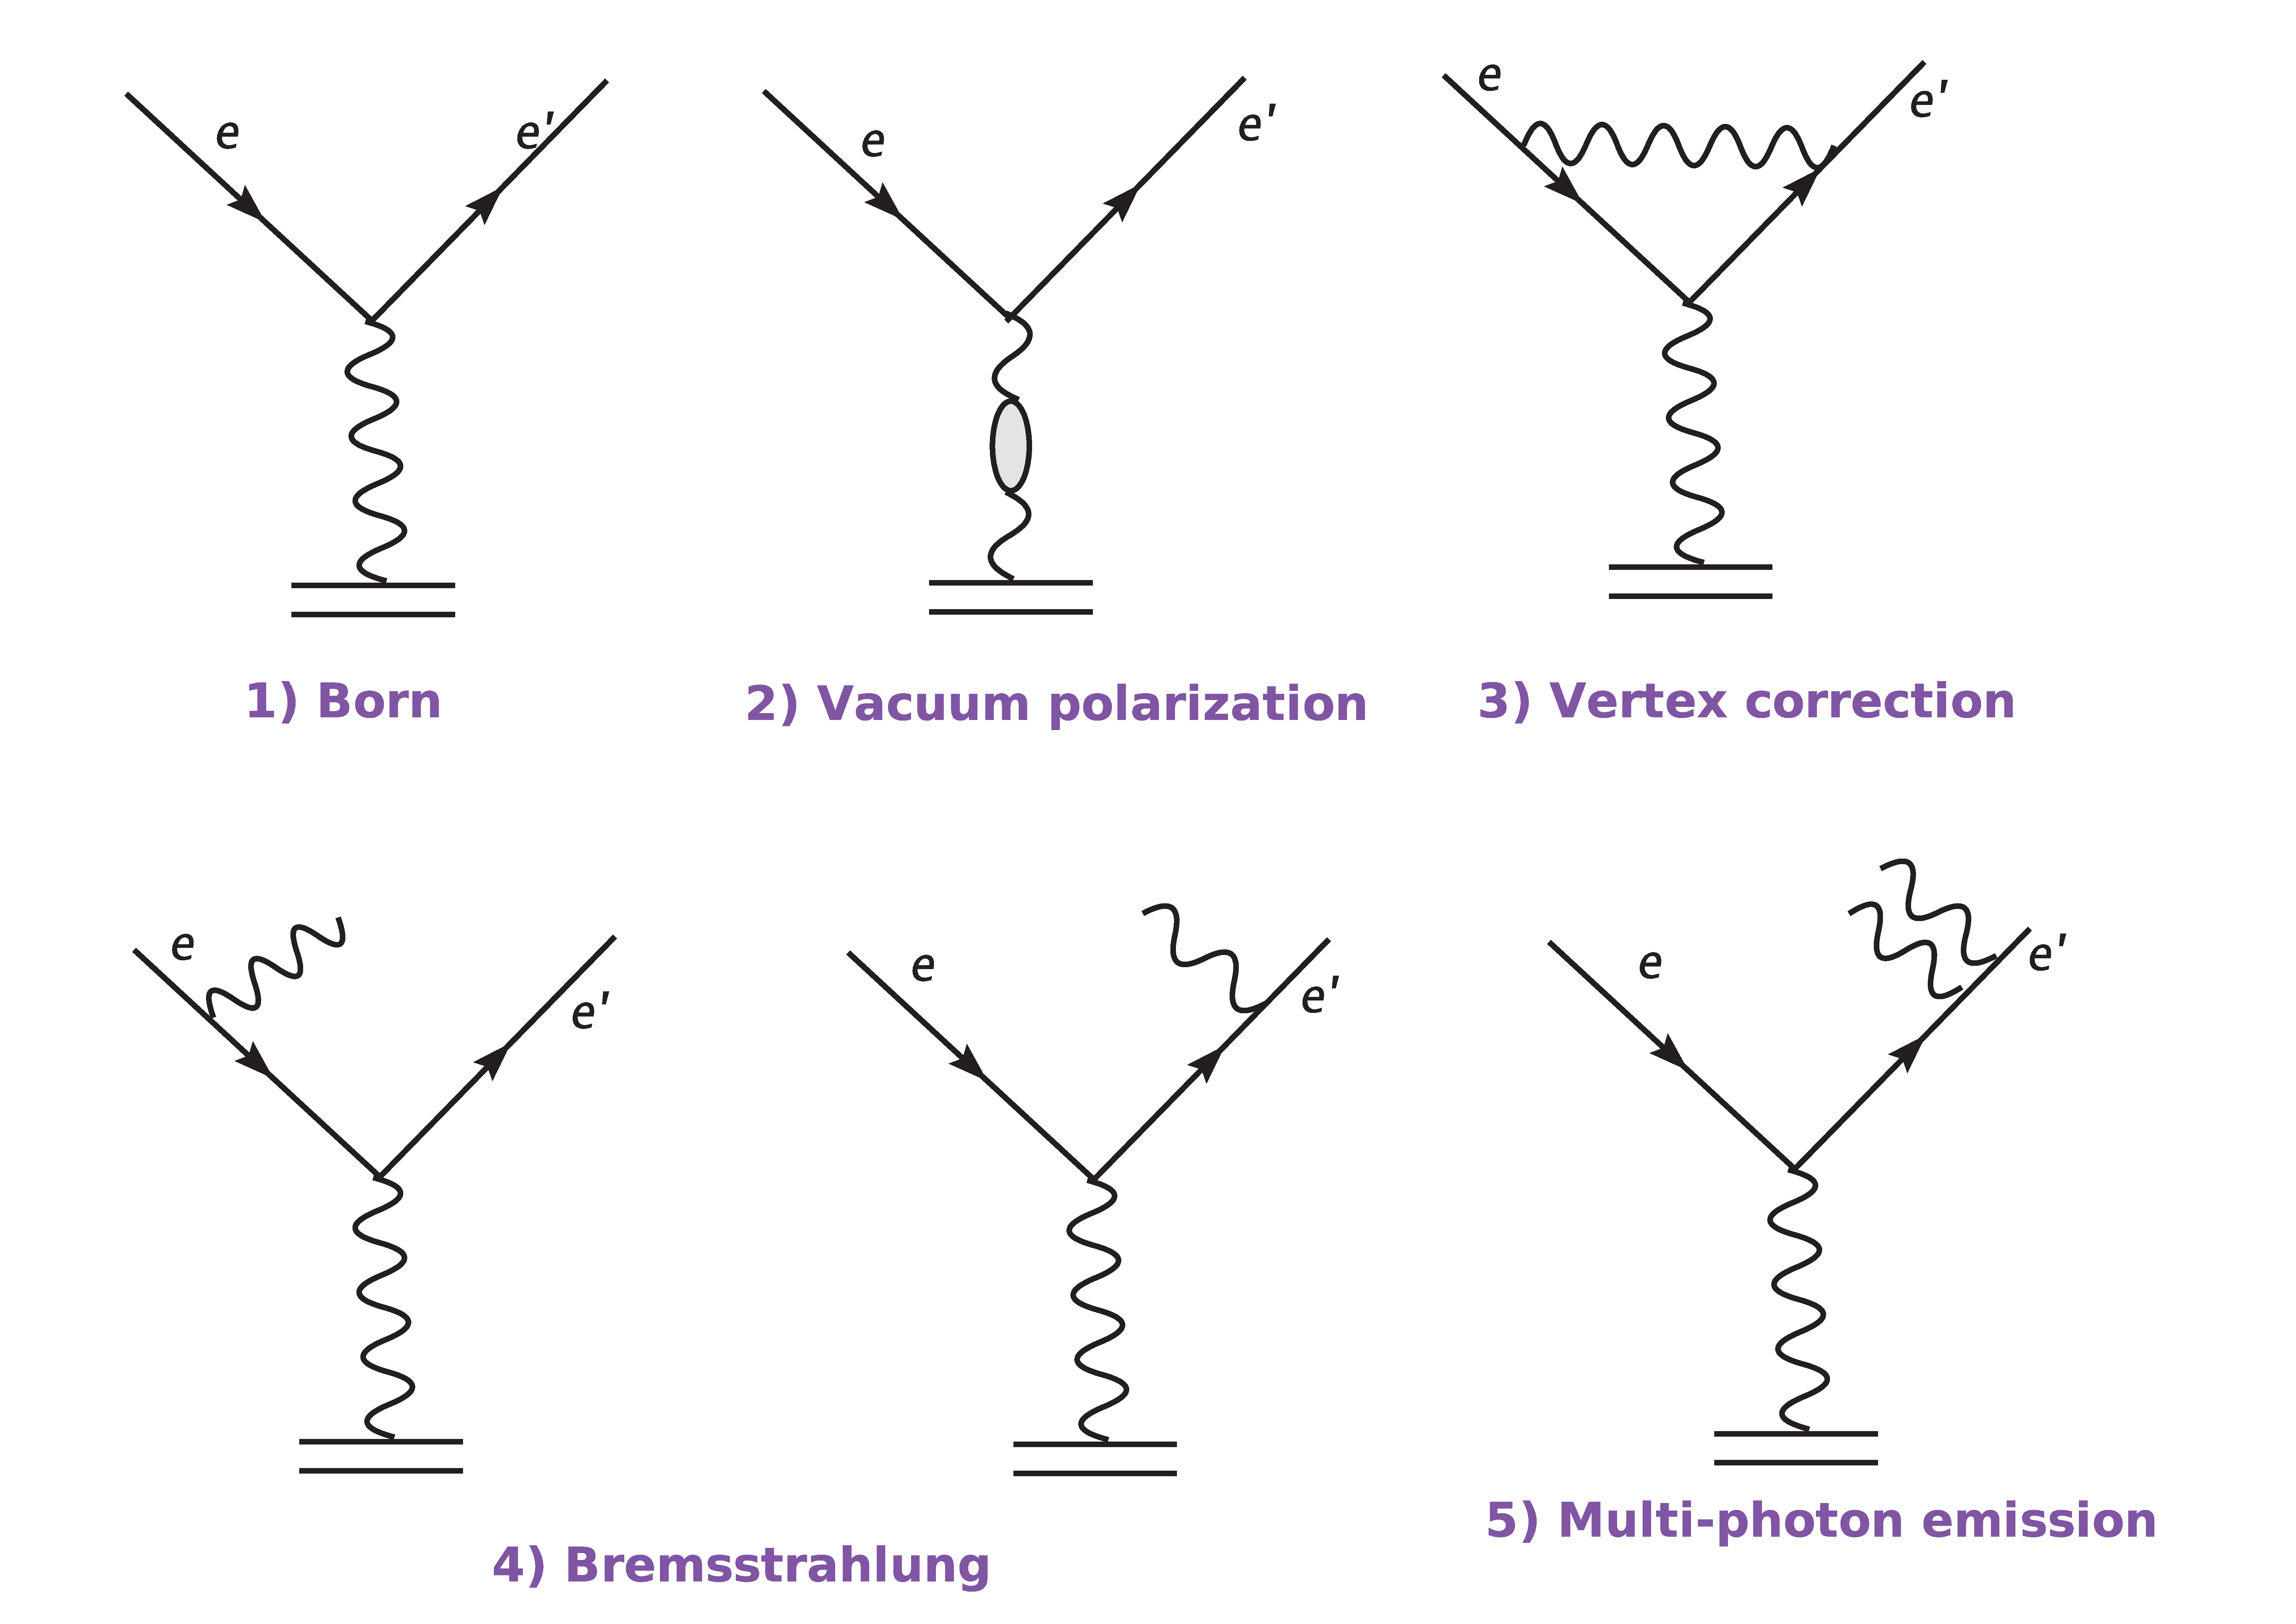
\includegraphics[angle=0,width=0.8\textwidth]{./figures/physics/radiated_feymann}
  \caption[Feynman diagrams for radiation effect]{Feynman diagrams for radiation effect in inclusive lepton-nucleon scattering. Only the lowest orders are shown here.}
  \label{rad_feynm}
 \end{center}
\end{figure} 
 The electron-nucleon scattering process can be modelled by one-photon-exchange-approximation (OPEA), where the electron and the nucleon interact by exchanging one virtual photon. The inclusive cross section of the process is called the Born cross section. There are higher order processes, called radiative effects, contributing to the measured cross sections, as shown in Fig.~\ref{rad_feynm}. The experimental raw cross section is named as the radiated cross section, which has to be corrected to obtain the experimental Born cross section: 
 \begin{equation}
  \sigma^{EX}_{Born} = \frac{\sigma^{Model}_{Born}}{\sigma^{Model}_{rad}}\cdot\sigma^{EX}_{rad},
 \end{equation}
where $\sigma^{Model}_{Born}$ and $\sigma^{Model}_{rad}$ are the Born and radiated cross section calculated from the model, while $\sigma^{EX}_{Born}$ and $\sigma^{EX}_{rad}$ are the Born and radiated cross sections measured from the experiment. The ratio term is generally called the radiative correction factor. 
 
  The radiation effects contain the external radiation and the internal radiation. The external radiation, including external bremsstrahlung and ionization, happens when the incoming or the outgoing electron radiates a real photon when it interacts with the nuclear medium other than the target nucleon. This effect mainly depends on the material and thickness of the target. The internal radiation contains the soft processes, such as internal bremsstrahlung, and the hard processes, such as vacuum polarization, vertex corrections and multiple-photon exchange. The initial and final energies of the electron are modified during those processes, which causes the measured cross section to deviate from the Born cross section.

   The idea of radiative correction is carefully discussed in~\cite{mo_sai_rad, stein_radiation}, and a radiative correction package, RadCor, was developed based on this idea~\cite{karl_thesis,hyao_thesis}. Peak approximation method was used in the package to reduce the CPU time of the radiated cross section calculation. Important subroutines in this package have been migrated to XEMC. 
   
 \section{Performance} 
  In this section, the cross sections calculated from XEMC with the QE-XEM model and the DIS-F1F209 model are directly compared with previous experiment data stored in the QES-Archive~\cite{qe_donal} (Fig.~\ref{xs_achieve_com1} and Fig.~\ref{xs_achieve_com2}) as well as the E02-019 data (Fig.~\ref{xs_nadia_b1} and Fig.~\ref{xs_nadia_b2}). Overall, the model and the data agree nicely. The performance of the radiative correction was examined with the E02-019 data of which the target configurations were known. From Fig.~\ref{xs_nadia_r1} and Fig.~\ref{xs_nadia_r2}, the radiated cross sections from XEMC agree well with the data above the QE region. At $x_{bj}<1$ a small deviation can be seen due to the use of the peak approximation method. The E08-014 data is well above the QE peak so the deviation wasn't important. 
\begin{figure}[!h]
  \begin{center}
    \subfloat[$\mathrm{^{2}D}$ from Arrington 1995]{
      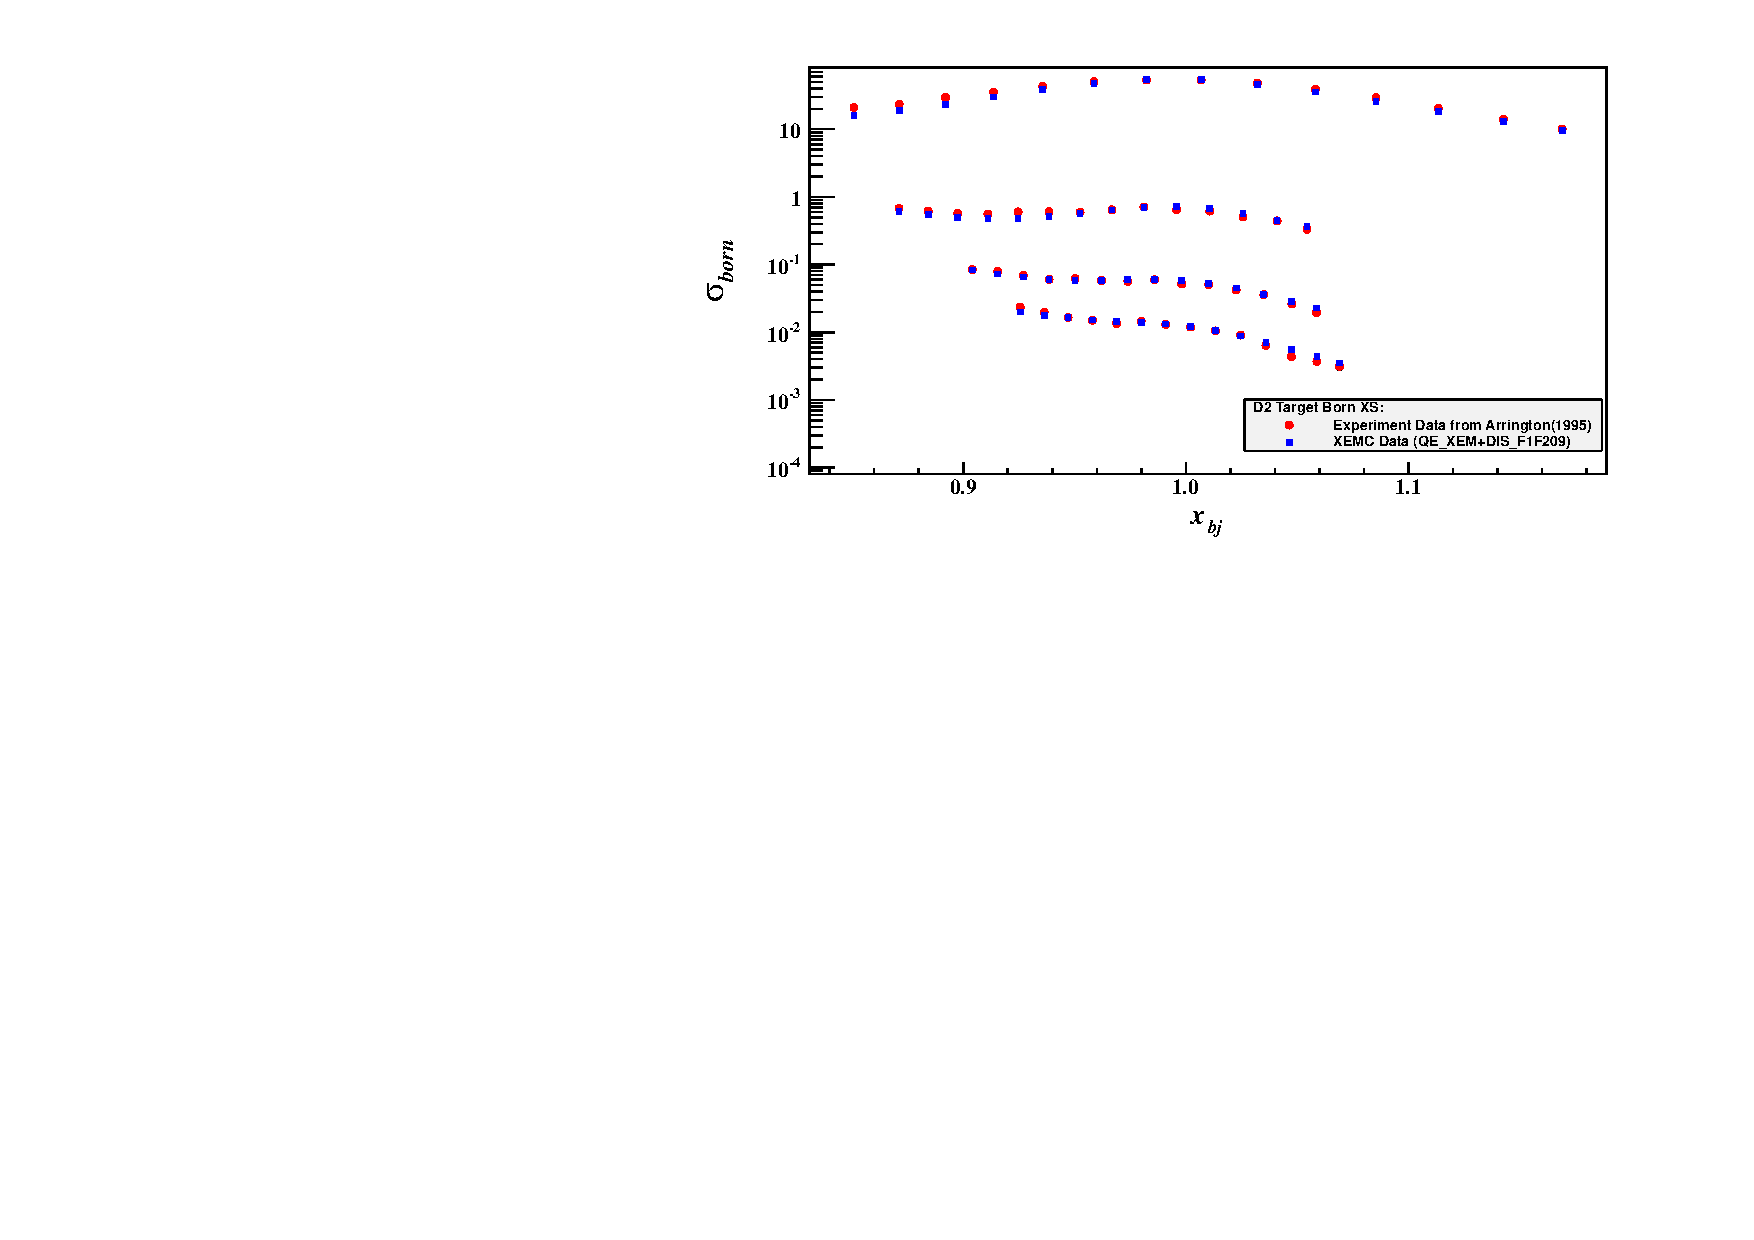
\includegraphics[type=pdf,ext=.pdf,read=.pdf,width=0.9\textwidth]{./figures/xemc/QEA_D2_Jan16_Born_Com_Arrington_1995}
    }
    \\
     \subfloat[$\mathrm{^{3}He}$ from Day 1979]{
      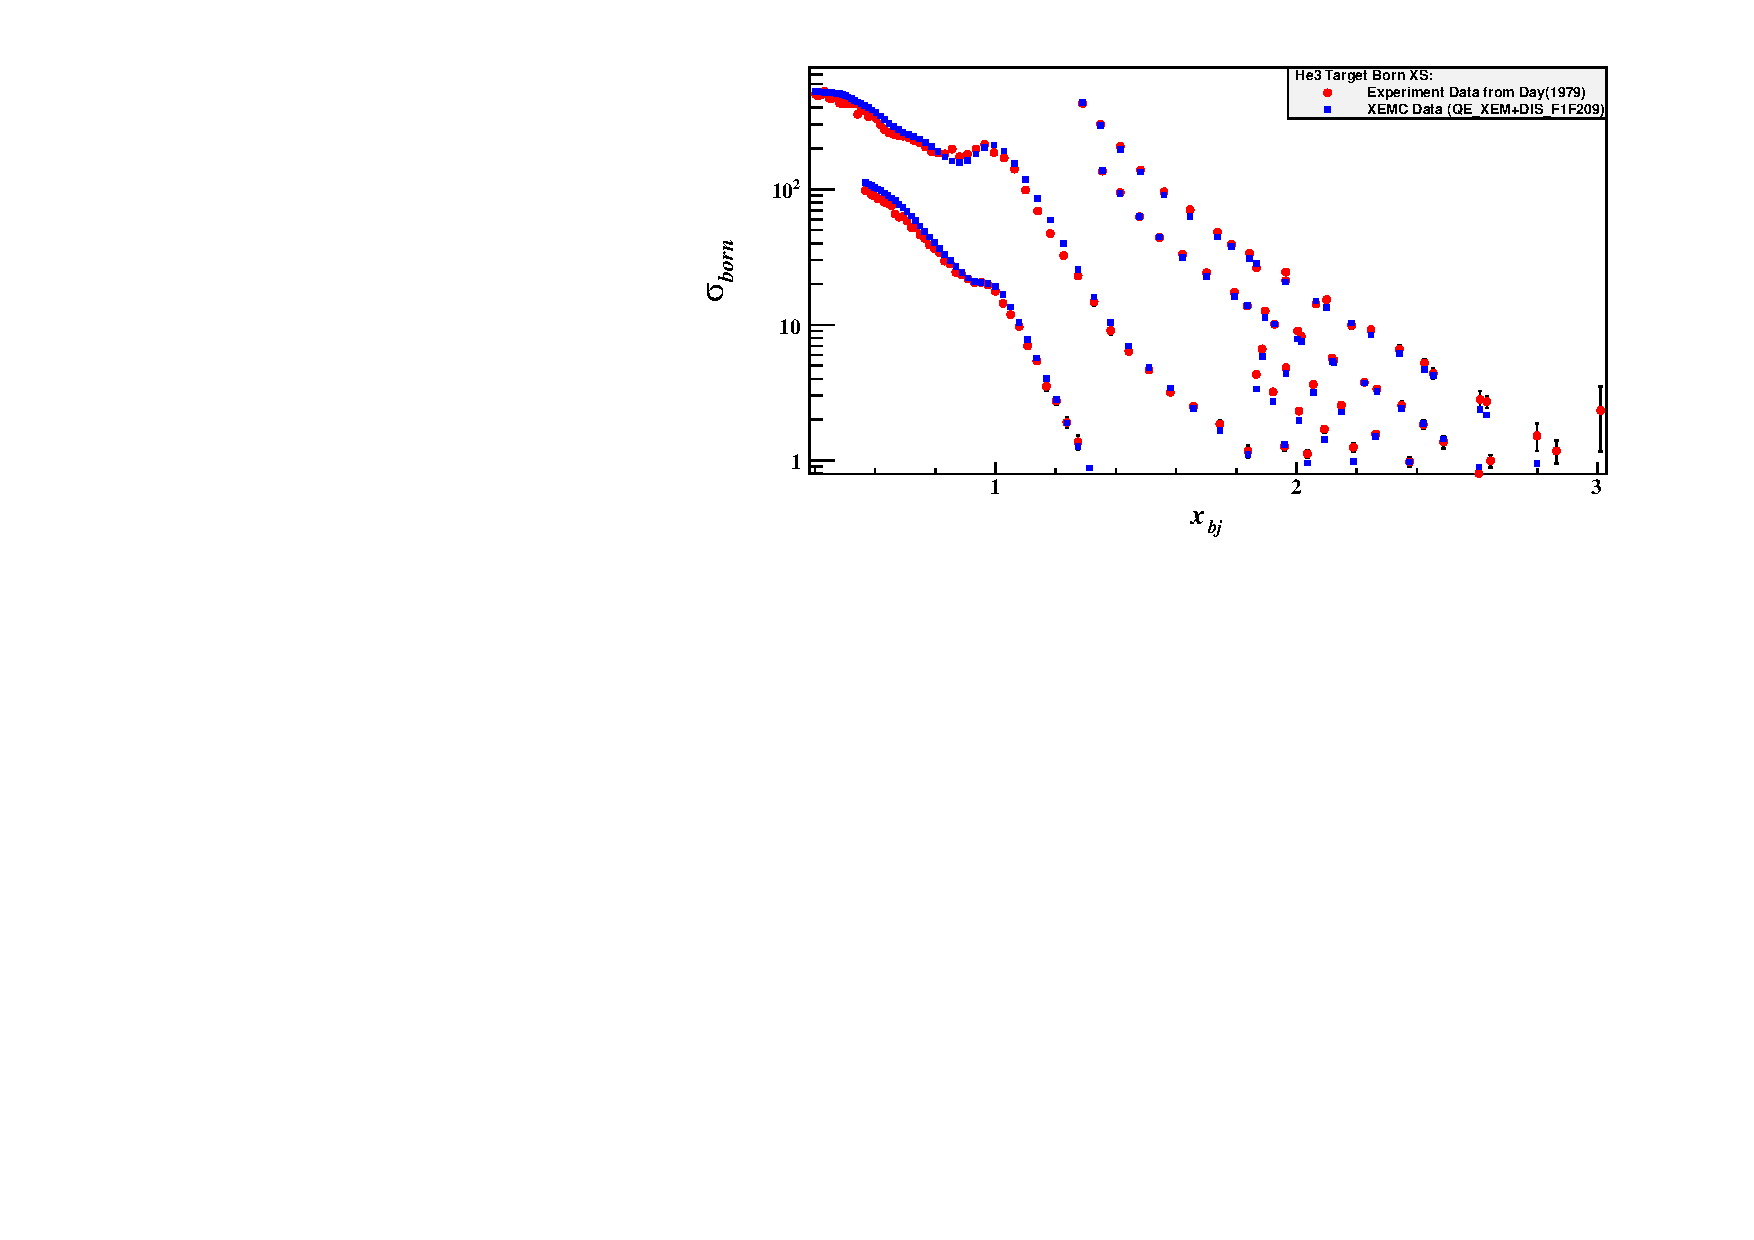
\includegraphics[type=pdf,ext=.pdf,read=.pdf,width=0.8\textwidth]{./figures/xemc/QEA_He3_Jan16_Born_Com_Day_1979}
    }
     \caption[Comparing XEMC models and experiment data for $\mathrm{^{2}D}$ and $\mathrm{^{3}He}$]{\footnotesize{Comparing XEMC models and experiment data for $\mathrm{^{2}D}$ and $\mathrm{^{3}He}$. Data is from QES-Archive~\cite{qe_donal}.}}
    \label{xs_achieve_com1}
  \end{center}
\end{figure}
\begin{figure}[!h]
  \begin{center}
     \subfloat[$\mathrm{^{4}He}$ from Meziani 1992]{
      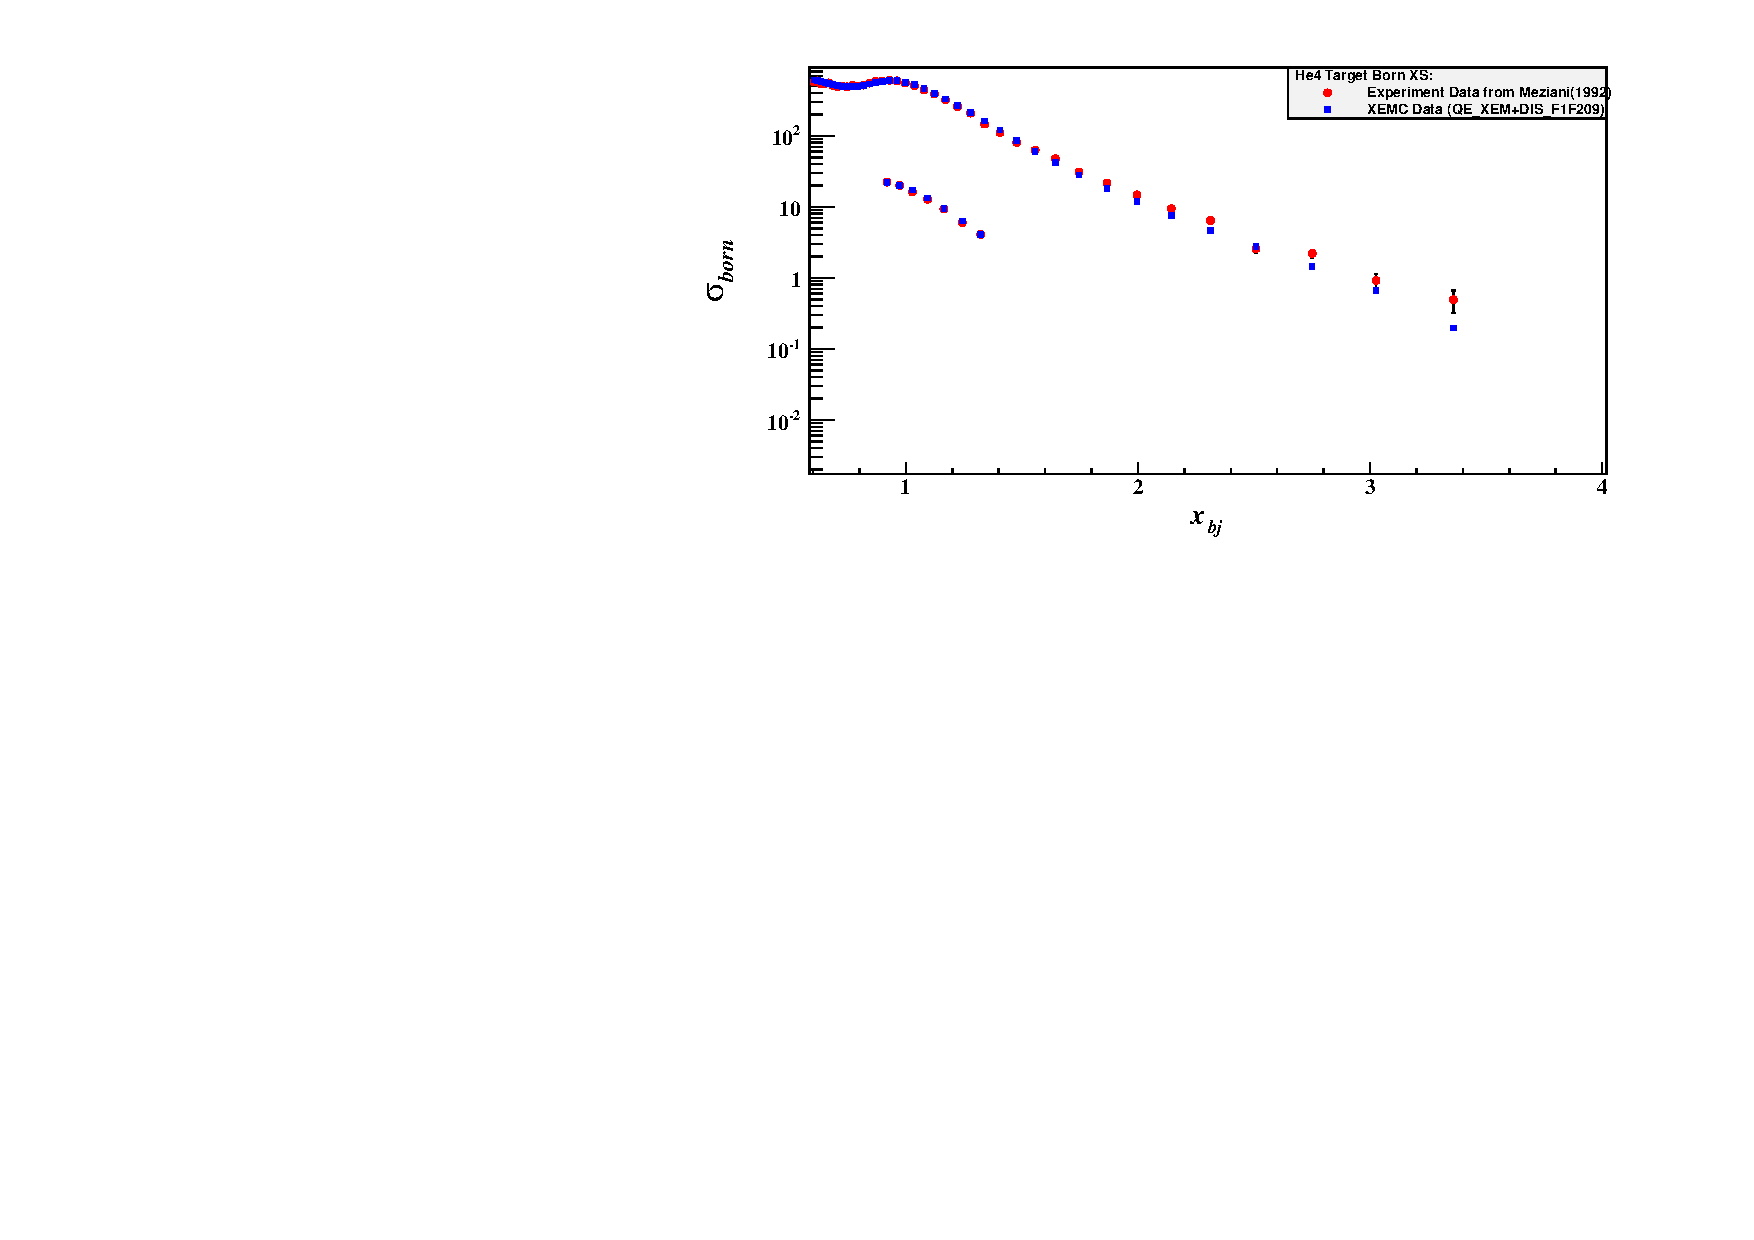
\includegraphics[type=pdf,ext=.pdf,read=.pdf,width=0.9\textwidth]{./figures/xemc/QEA_He4_Jan16_Born_Com_Meziani_1992}
      \label{target_run1}
    }
    \\
     \subfloat[$\mathrm{^{12}C}$ from Arrington 1998]{
      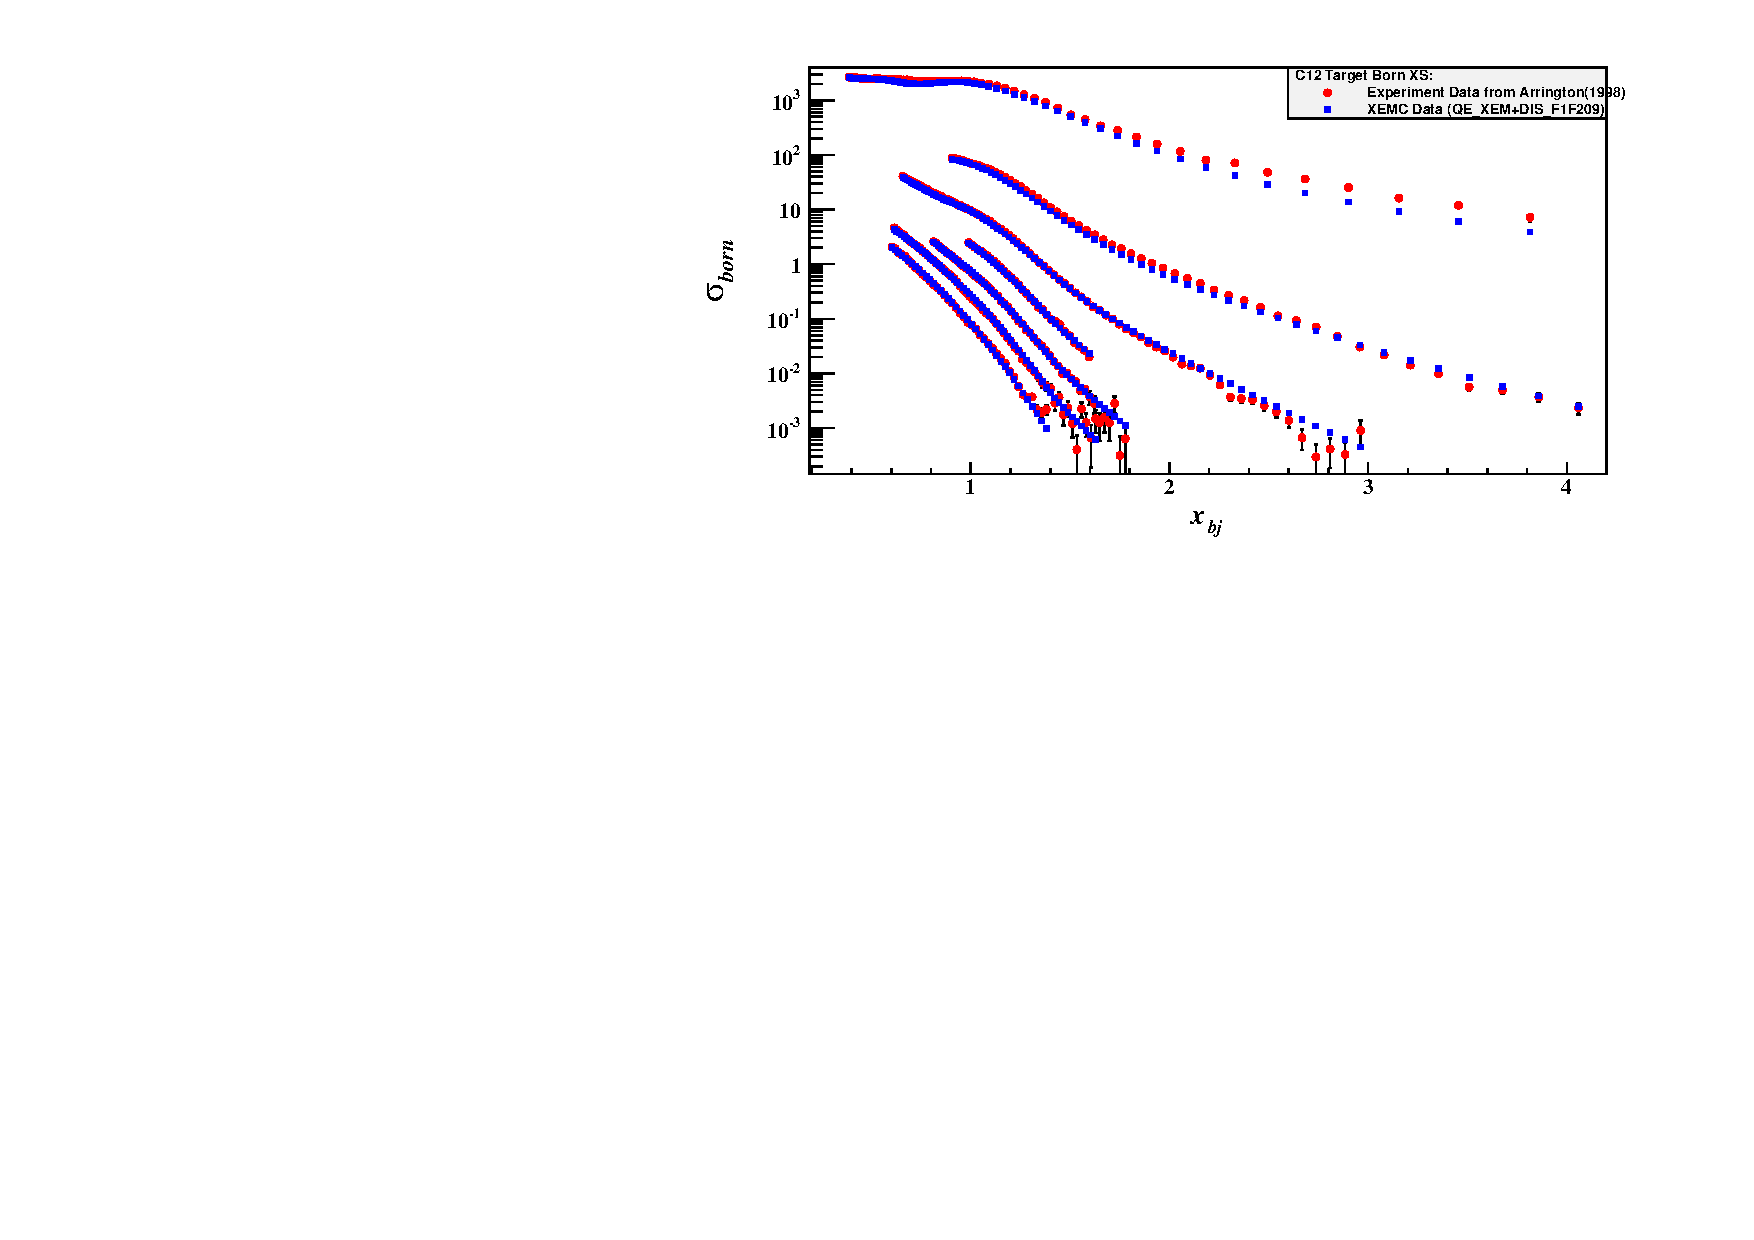
\includegraphics[type=pdf,ext=.pdf,read=.pdf,width=0.9\textwidth]{./figures/xemc/QEA_C12_Jan16_Born_Com_Arrington_1998}
    }
 \caption[Comparing XEMC models and experiment data for $\mathrm{^{4}He}$ and $\mathrm{^{12}C}$]{\footnotesize{Comparing XEMC models and experiment data for $\mathrm{^{4}He}$ and $\mathrm{^{12}C}$. Larger deviation can be seen in $\mathrm{^{12}C}$ data low $\mathrm{Q^{2}}$. Data is from QES-Archive~\cite{qe_donal}.}}   
  \label{xs_achieve_com2}
  \end{center}
\end{figure}
\begin{figure}[!h]
  \begin{center}
    \subfloat[$\mathrm{^{3}He}$ Born cross section]{
      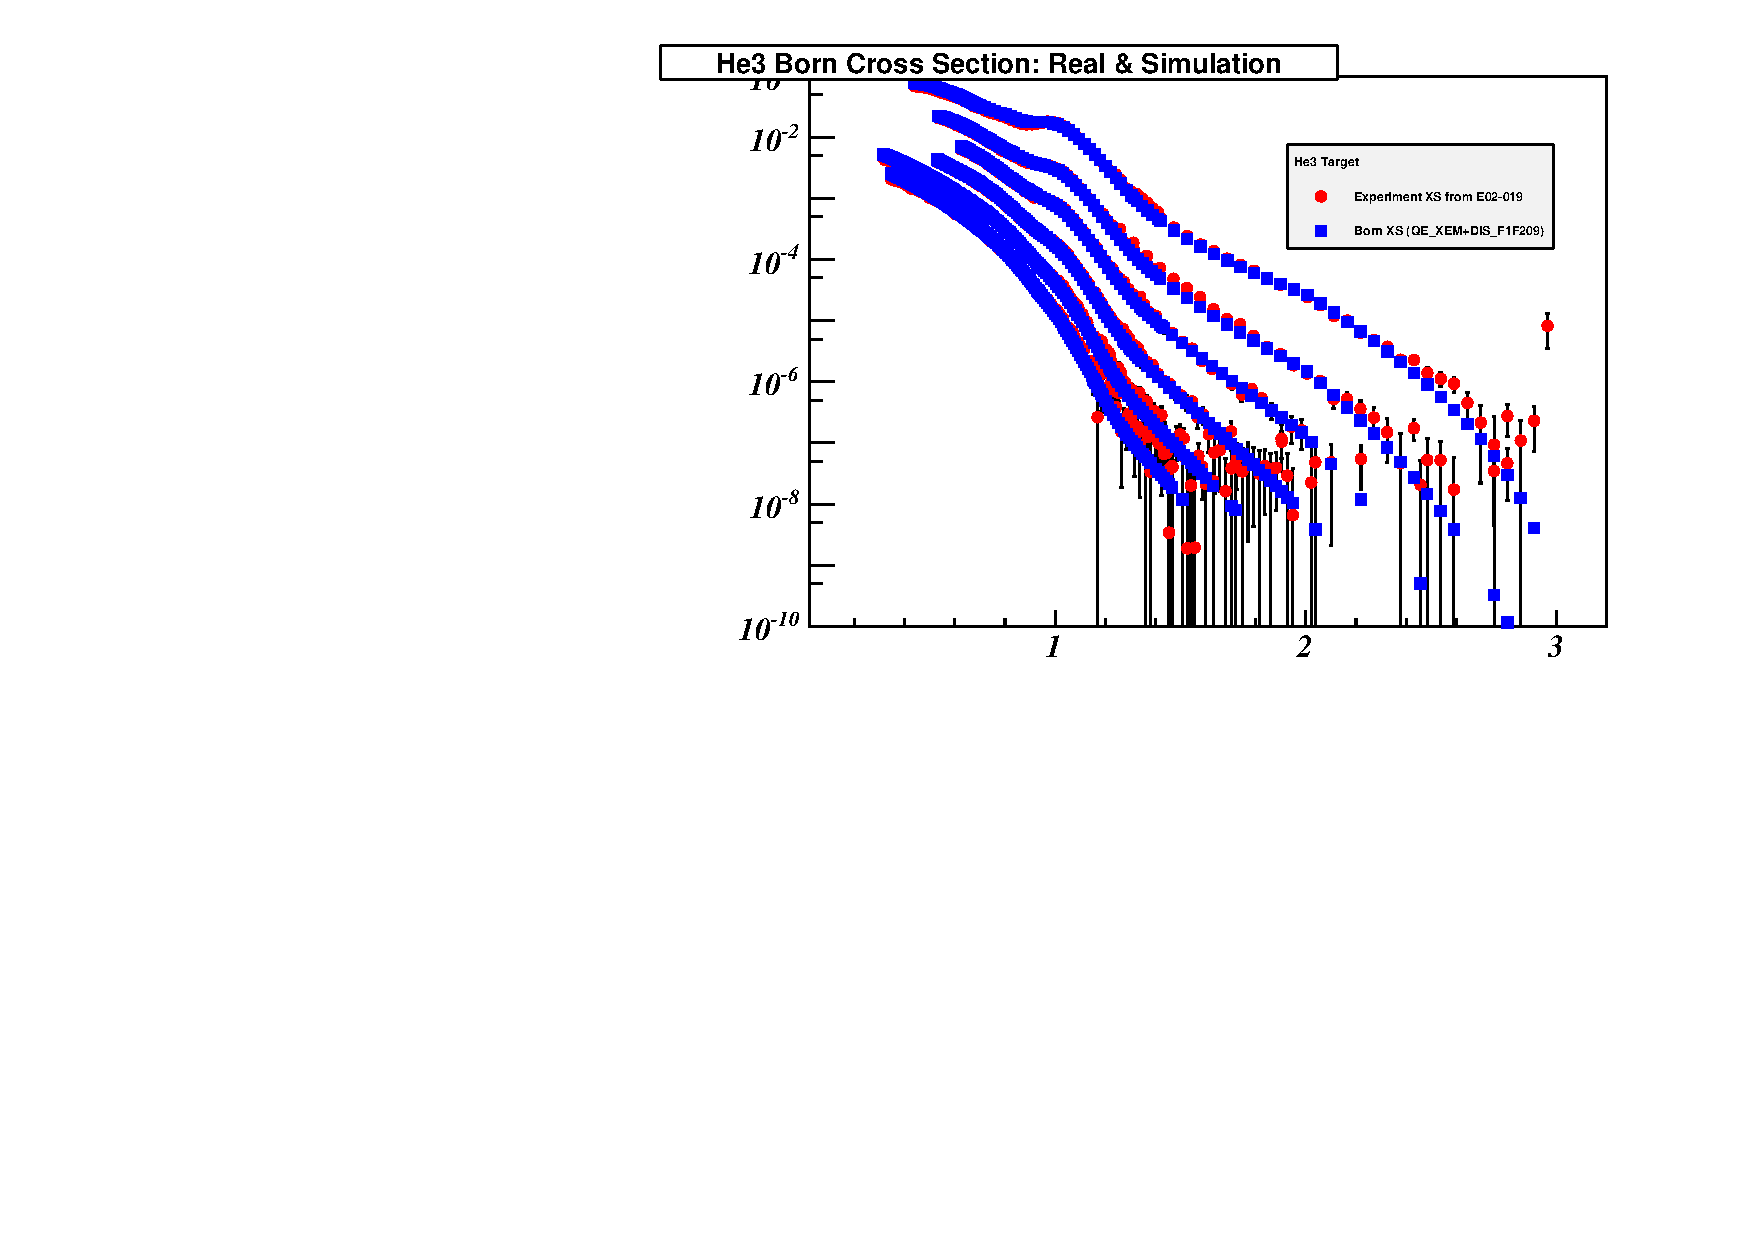
\includegraphics[type=pdf,ext=.pdf,read=.pdf,width=0.9\textwidth]{./figures/xemc/He3_XEMC_Born_Com}
      \label{xs_nadia_b1}
    }
    \\
       \subfloat[$\mathrm{^{3}He}$ radiated cross section]{
      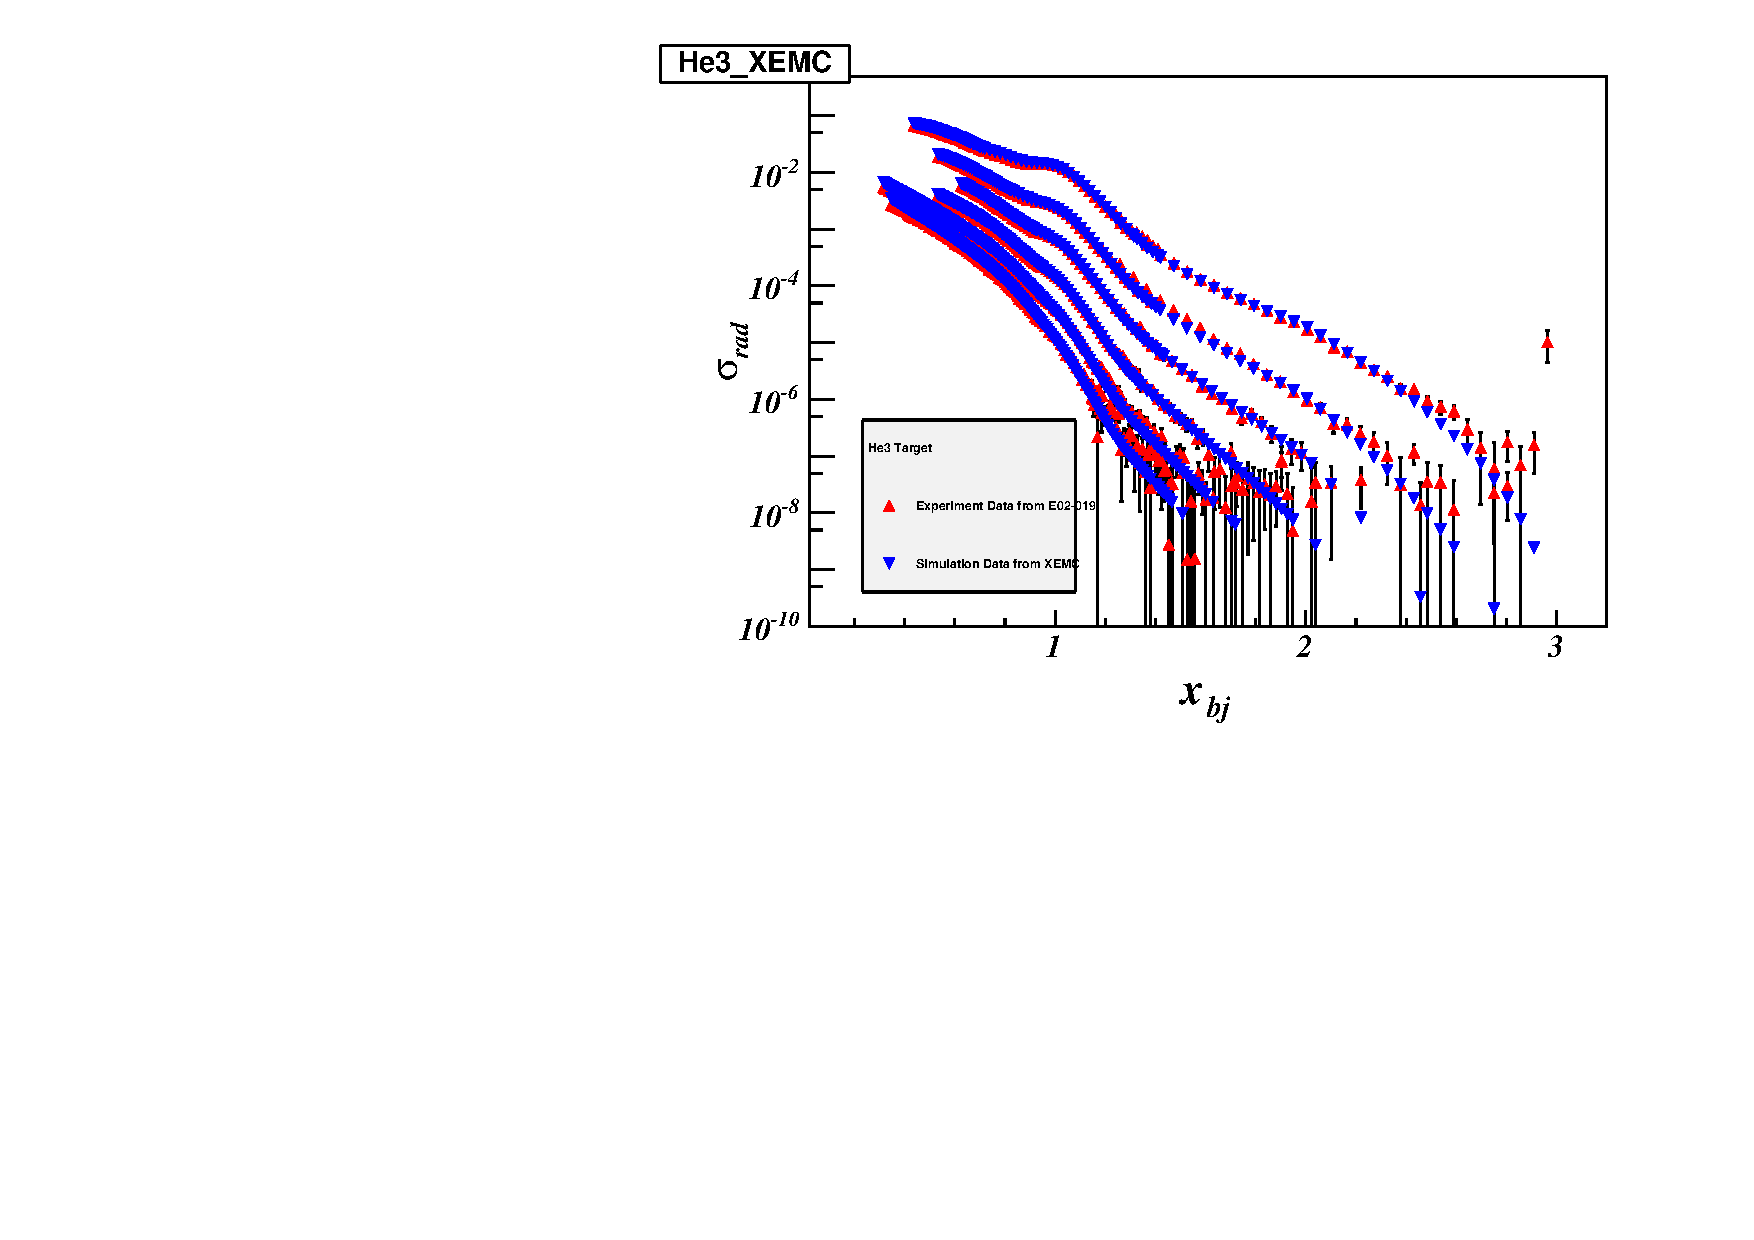
\includegraphics[type=pdf,ext=.pdf,read=.pdf,width=0.9\textwidth]{./figures/xemc/He3_XEMC_Rad_Com}
      \label{xs_nadia_r1}
    }
    \caption[Comparing $\mathrm{^{3}He}$ cross sections from E02-019 and calculated in XEMC]{\footnotesize{Comparing $\mathrm{^{3}He}$ cross sections from E02-019~\cite{nadia_thesis} and calculated in XEMC, where top and bottom plots are the Born and radiated cross section, respectively. The thickness of the target and the configuration of the target system are included~\cite{nadia_thesis}.}}
    \label{xs_nadia_com1}
  \end{center}
\end{figure}
\begin{figure}[!h]
  \begin{center}
     \subfloat[$\mathrm{^{12}C}$ Born cross section]{
      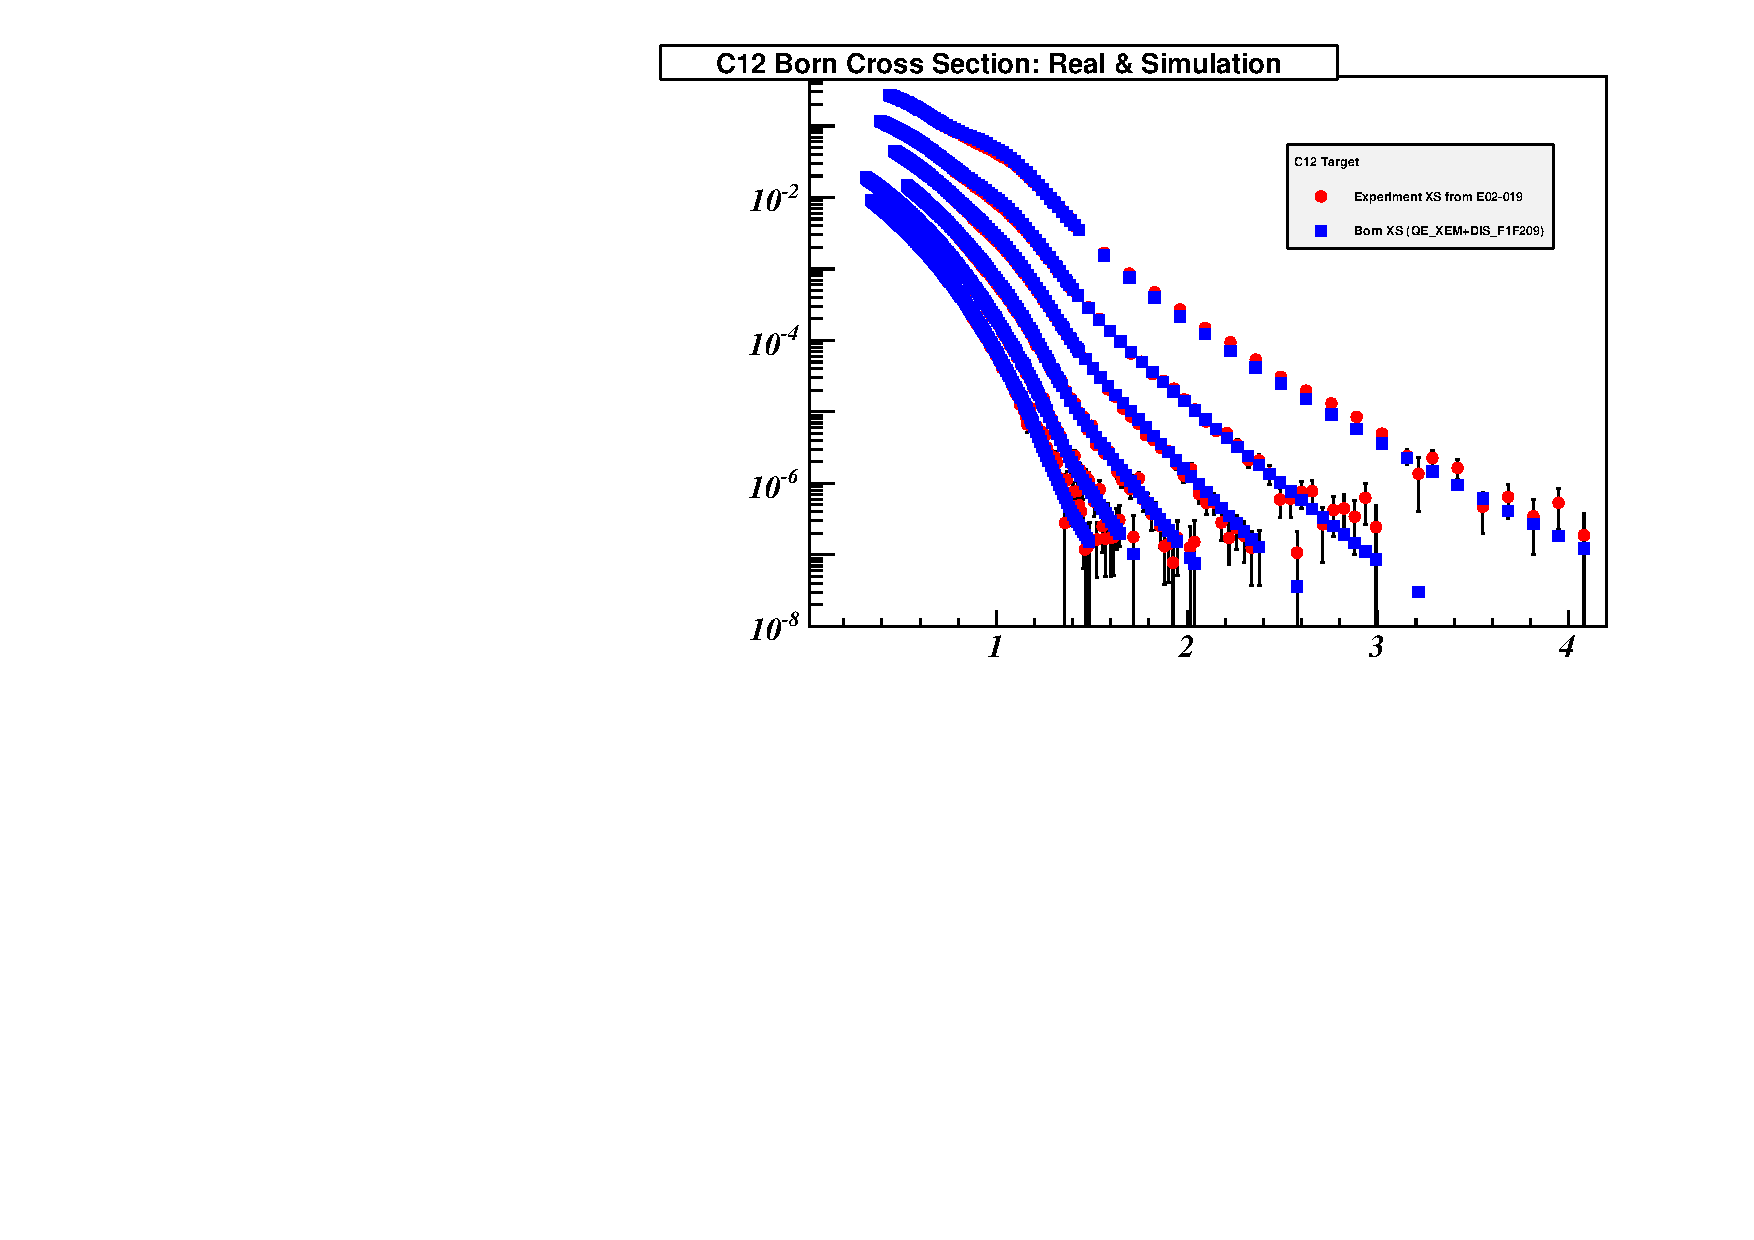
\includegraphics[type=pdf,ext=.pdf,read=.pdf,width=0.9\textwidth]{./figures/xemc/C12_XEMC_Born_Com}
      \label{xs_nadia_b2}
    }
    \\
     \subfloat[$\mathrm{^{12}C}$ radiated cross section]{
      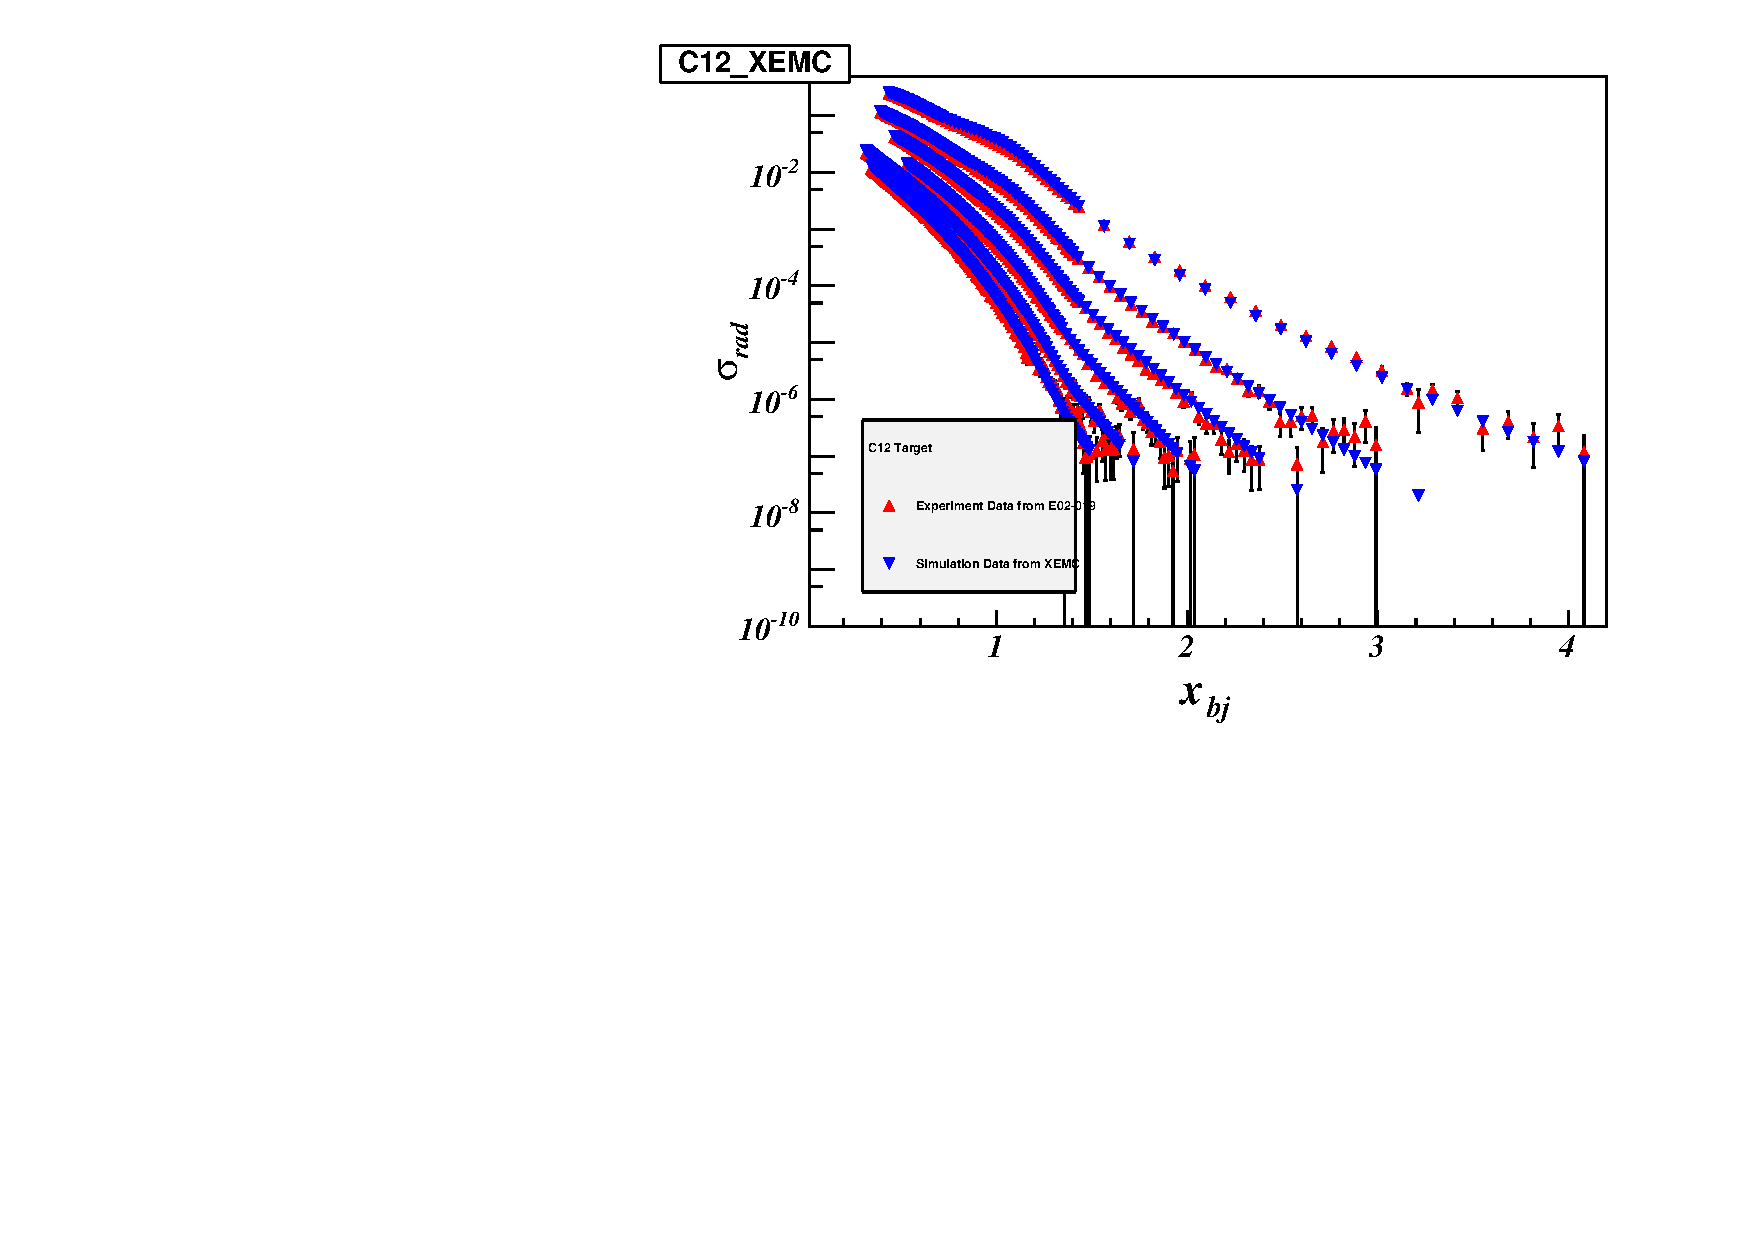
\includegraphics[type=pdf,ext=.pdf,read=.pdf,width=0.9\textwidth]{./figures/xemc/C12_XEMC_Rad_Com}
      \label{xs_nadia_r2}
    }
    \caption[Comparing $\mathrm{^{12}C}$ cross sections from E02-019 and calculated in XEMC]{\footnotesize{Comparing $\mathrm{^{12}C}$ cross sections from E02-019~\cite{nadia_thesis} and calculated in XEMC, where top and bottom plots are the Born and radiated cross section, respectively. The thickness of the target and the configuration of the target system are included~\cite{nadia_thesis}.}}
    \label{xs_nadia_com2}
  \end{center}
\end{figure}

\newpage
\section{Examples}
 An example to use the XEMC package is given in this section. 
% \newpage 
 \begin{lstlisting}
#include "XEMC.h"
int main(int argc,char** argv){
	XEMC* Event = new XEMC(); //Create a XEMC event
	//Target
	const int A = 12, Z = 6;    
	TString Target_Name = "C12";
    	Event->Init(Form("./input/%s_Input.dat",Target_Name.Data()));	
 	//Kinematic setting	
	double E0 = 3.356;    //GeV
	double Ep = 2.505;    //GeV/c
	double Theta = 25.00; //Degree
		
	//Calculate XS for the event
	int err = Event->Process(E0,Ep,Theta,A,Z);	
	if(err>=0){ //Return values
		double xs_rad  = Event->XS_Rad();
		double xs_qe   = Event->XS_QE();
		double xs_dis  = Event->XS_DIS();
		double xs_Born = Event->XS_Born();
	}
	//Print Out
	cerr<<Form("For %s Target, E0=%5.3f GeV, Ep=%5.3f GeV, Theta=%5.3f:",Target_Name.Data(), E0, Ep, Theta)<<endl;
	cerr<<Form("    XS_Born=%e, XS_QE=%e, XS_DIS=%e, XS_Rad=%e",
                    xs_Born, xs_qe, xs_dis, xs_rad)<<endl;	
	
	delete Event; //Release memory
}
\end{lstlisting}
\chapter{Momentum Correction in HRS-R}
  Each HRS is composed of a dipole and three quadrupoles in the order of Q1, Dipole, Q2 and Q3. Four magnets typically have the same central momentum value. With the focal plane quantities provided by the VDC tracking, a HRS optics matrix reconstructs $\delta p$, $y_{tg}$, $\theta_{tg}$, and $\phi_{tg}$, the target plane quantities to describe an event at the reaction point. As discussed in Section 3.3, during the E08-014, the field of the Q3 magnet on HRS-R (RQ3) was scaled to 87.72\% of its normal value, and the transportation of particles in the HRS-R had been changed. While the matrix elements of $y_{tg}$, $\theta_{tg}$, and $\phi_{tg}$ have been properly optimized (see Section 4.3), the momentum matrix (the D-terms) could not be calibrated since the momentum calibration data was not available in the quasielastic region. It requires an additional correction to get the right value of $\delta p$. In this section, a method will be introduced to correct the $\delta p$ on HRS-R with the SAMC data and the SNAKE model~\cite{snack_lerose}.
 
 In the Hall-A Single Arm Monte Carlo tool (SAMC), each HRS magnet's transportation from the entrance to the exit is simulated in the SNAKE model as a series of forward transportation functions (FWDs). For example, the quantities at the Q1 entrance, $x_{Q1}^{en}$, $y_{Q1}^{en}$, $\theta_{Q1}^{en}$, $\phi_{Q1}^{en}$, and $l_{Q1}^{en}$ can be directly deduced from the target plane quantities via the linear transportation; and the quantities at the Q1 exit, $x_{Q1}^{ex}$, $y_{Q1}^{ex}$, $\theta_{Q1}^{ex}$, $\phi_{Q1}^{ex}$, and $l_{Q1}^{ex}$ can be calculated with their corresponding FWDs with the quantities at the entrance as inputs. These quantities at the Q1 exit are equal to the quantities at the dipole entrance and can be further used to calculate the quantities at the dipole exit; so on and so forth. The focal plane quantities, $x_{fp}$, $y_{fp}$,$\theta_{fp}$, and $\phi_{fp}$, are given by the FWDs of Q3. The focal plane quantities are then smeared with the resolution of the HRS VDCs defined in the simulation.
 
  Similar to the HRS optics matrix, a set of backward polynomial functions (BWDs) directly calculate each target plane quantity with the four focal plane quantities as inputs.
  
 To simulate the HRS-R setting during this experiment, new FWDs were generated for the RQ3 with the mis-matching field, named as $\mathrm{FWD^{Q3}_{mis}}$, and they replaced the FWDs with the normal field setting ($\mathrm{FWD^{Q3}_{norm}}$) in the simulation. Besides, two sets of new BWDs were also produced by SNAKE to describe the RQ3. The first set ($\mathrm{BWD_{mis}^{D}}$) has the correct reconstructions of all target plane quantities. It simulates the optics matrix on HRS-R with all terms being optimized. The second set ($\mathrm{BWD_{norm}^{D}}$) has also included the correct reconstructions of target plane quantities, except the one of $\delta p$ which was generated with the normal RQ3 field. This corresponds to the new optics matrix with the un-calibrated D-Terms.

 In SAMC, two groups of simulation events were generated with the same event seeds. The HRS-R in first group of events was simulated with $\mathrm{FWD^{Q3}_{mis}+BWD_{mis}^{D}}$, and the values of $\delta p$ in these events should be correctly reconstructed and are labelled as $\delta p_{cor}$. In the second group, the HRS-R was simulated with $\mathrm{FWD^{Q3}_{mis}+BWD_{norm}^{D}}$ which reconstructs incorrect values of $\delta p$, named as $\delta p_{in}$.
  
 In the real data, the error of the momentum reconstruction caused by using the un-calibrated D-terms can be studied by the difference of $\delta p_{cor}$ and $\delta p_{in}$ in the simulation data:
\begin{equation}
 \Delta\delta p = \delta p_{cor} - \delta p_{in},
\end{equation}
which can be specified by a correction function defined as:
\begin{eqnarray}
	 f(x_{fp}, \theta_{fp}, y_{fp}, \phi_{fp}) &=& \sum_{i=0}^{N_{A}}A_{i}x_{fp}^{i}+\sum_{j=0}^{N_{B}}B_{j}\theta_{fp}^{j}+\sum_{k=0}^{N_{C}}C_{k}y_{fp}^{k} \nonumber \\
                                   &+&\sum_{l=0}^{N_{D}}D_{l}\phi_{fp}^{l} +\sum_{m=0}^{N_{E}}E_{m}\delta p_{in}^{m},
\label{dp_corr_func}
\end{eqnarray}
where the first four terms are the polynomial functions of the focal plane quantities, and the last term is used to correct any high-order optics effects. The procedure to obtain the correction function from the simulation data is presented as follows. 

 First of all, the first term in Eq.~\eqref{dp_corr_func} is fitted with $x_{fp}$:
\begin{equation}
 \Delta\delta p(x_{fp}) = \delta p_{cor} - \delta p_{in} = \sum_{i=0}^{N_{A}}A_{i}x_{fp}^{i},
 \label{deltap_corr_xfp}
\end{equation}
which gives a new momentum value, $\delta p_{x_{fp}}=\delta p_{in}+\sum_{i=0}^{N_{A}}A_{i}x_{fp}^{i}$, and the residual error, $\Delta\delta p = \delta p_{cor}-\delta p_{x_{fp}}$, is further fitted with $\theta_{fp}$:
\begin{equation}
 \Delta\delta p(\theta_{fp}) = \delta p_{cor} - \delta p_{x_{fp}} = \sum_{j=0}^{N_{B}}B_{j}\theta_{fp}^{j},
 \label{deltap_corr_thetafp}
\end{equation}
which gives $\delta p_{\theta_{fp}}=\delta p_{x_{fp}}+\sum_{j=0}^{N_{B}}B_{j}\theta_{fp}^{j}$. Similar corrections are applied to $y_{fp}$, $\phi_{fp}$ and $\delta p_{in}$:
\begin{eqnarray}
 &&\Delta\delta p(y_{fp}) = \delta p_{cor} - \delta p_{\theta_{fp}} = \sum_{k=0}^{N_{C}}C_{k}y_{fp}^{k},\\
 &&\Delta\delta p(\phi_{fp})   = \delta p_{cor} - \delta p_{y_{fp}} = \sum_{l=0}^{N_{D}}D_{l}\phi_{fp}^{l},\\
 &&\Delta\delta p(\delta p_{in})   = \delta p_{cor} - \delta p_{\phi_{fp}} = \sum_{m=0}^{N_{E}}E_{m}\delta_{in}^{m}.
 \label{deltap_corr_deltap}
\end{eqnarray}
\begin{figure}[!ht]
  \begin{center}
    \subfloat[$\Delta\delta p(x_{fp})$ .vs. $x_{fp}$ and $\theta_{fp}$]{
      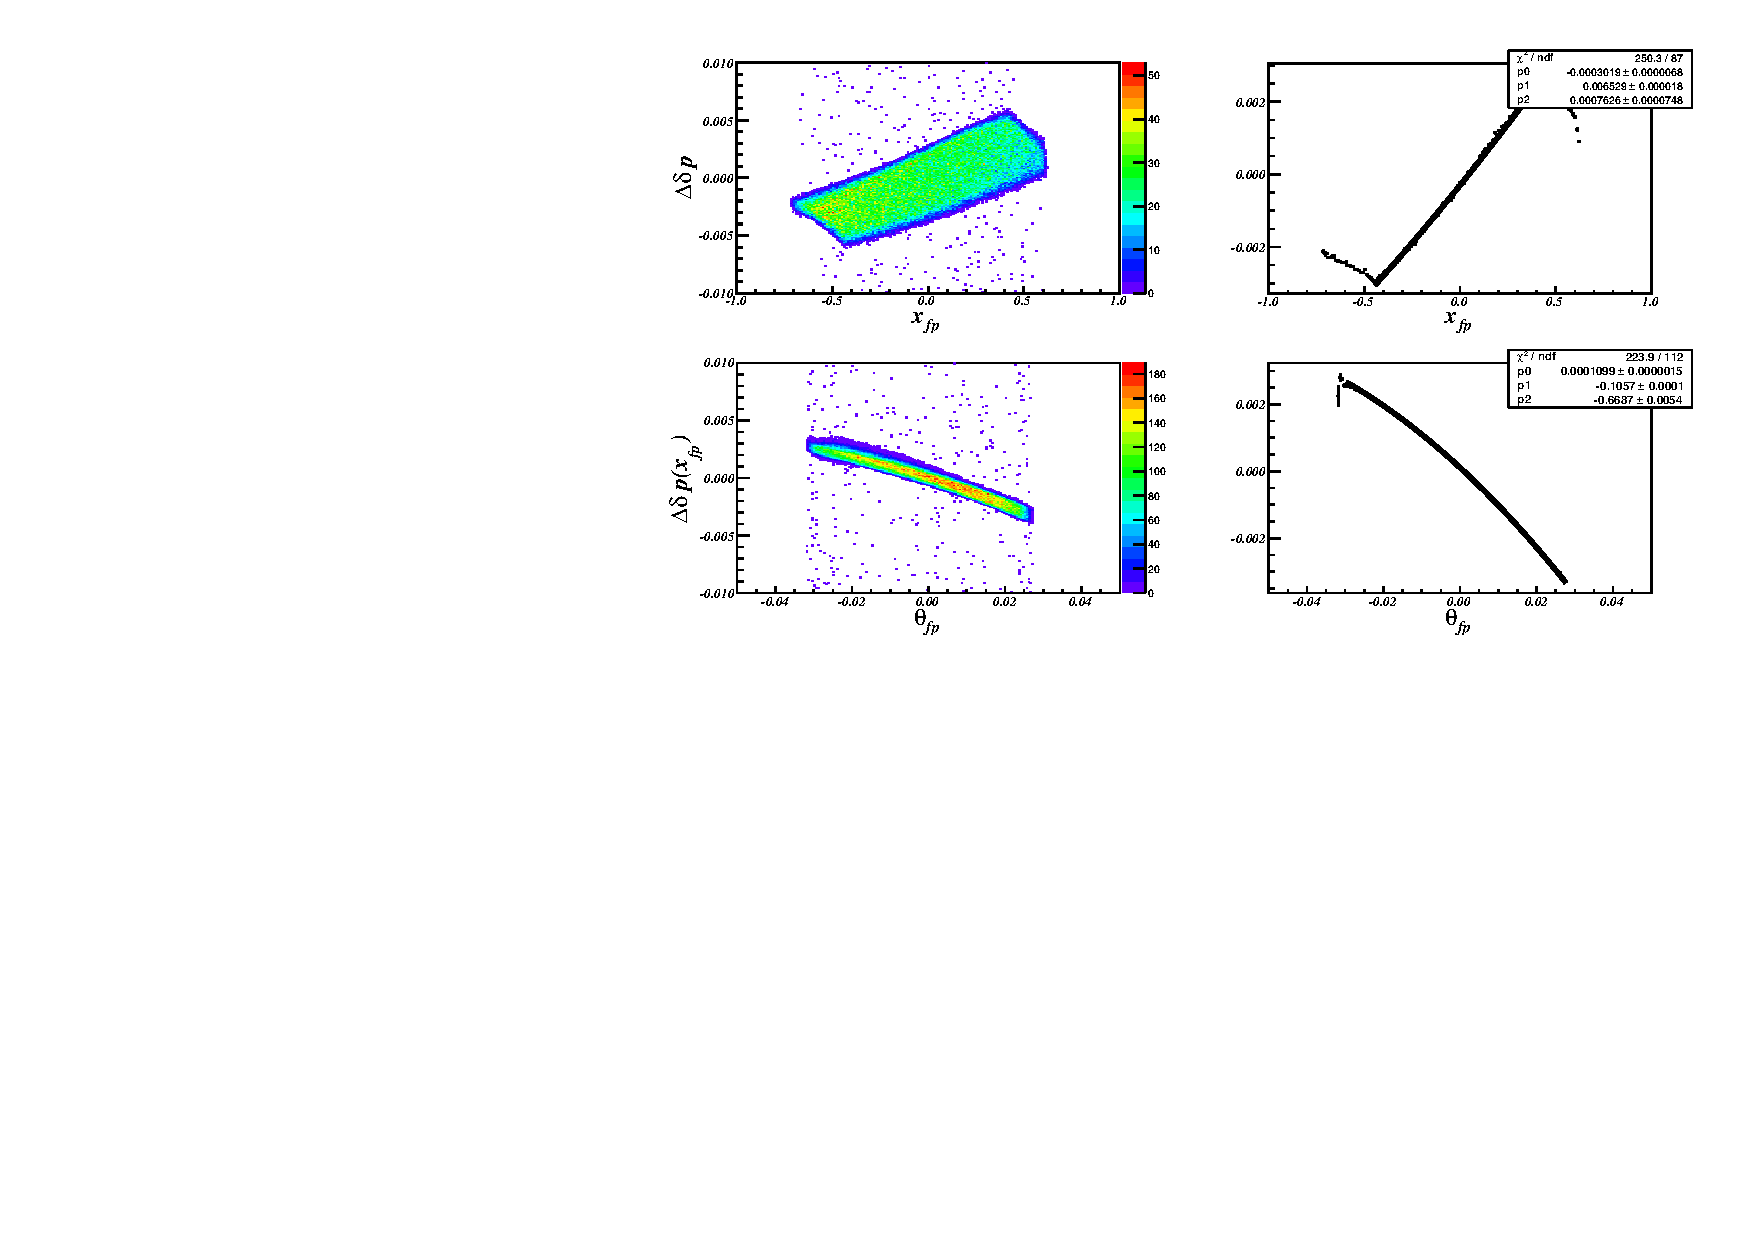
\includegraphics[type=pdf,ext=.pdf,read=.pdf,width=0.7\textwidth]{./figures/apend/DeltaCorr1_Kin31} 
    }
    \hfill
     \subfloat[$\Delta\delta p(y_{fp})$ .vs. $y_{fp}$ and $\phi_{fp}$]{
      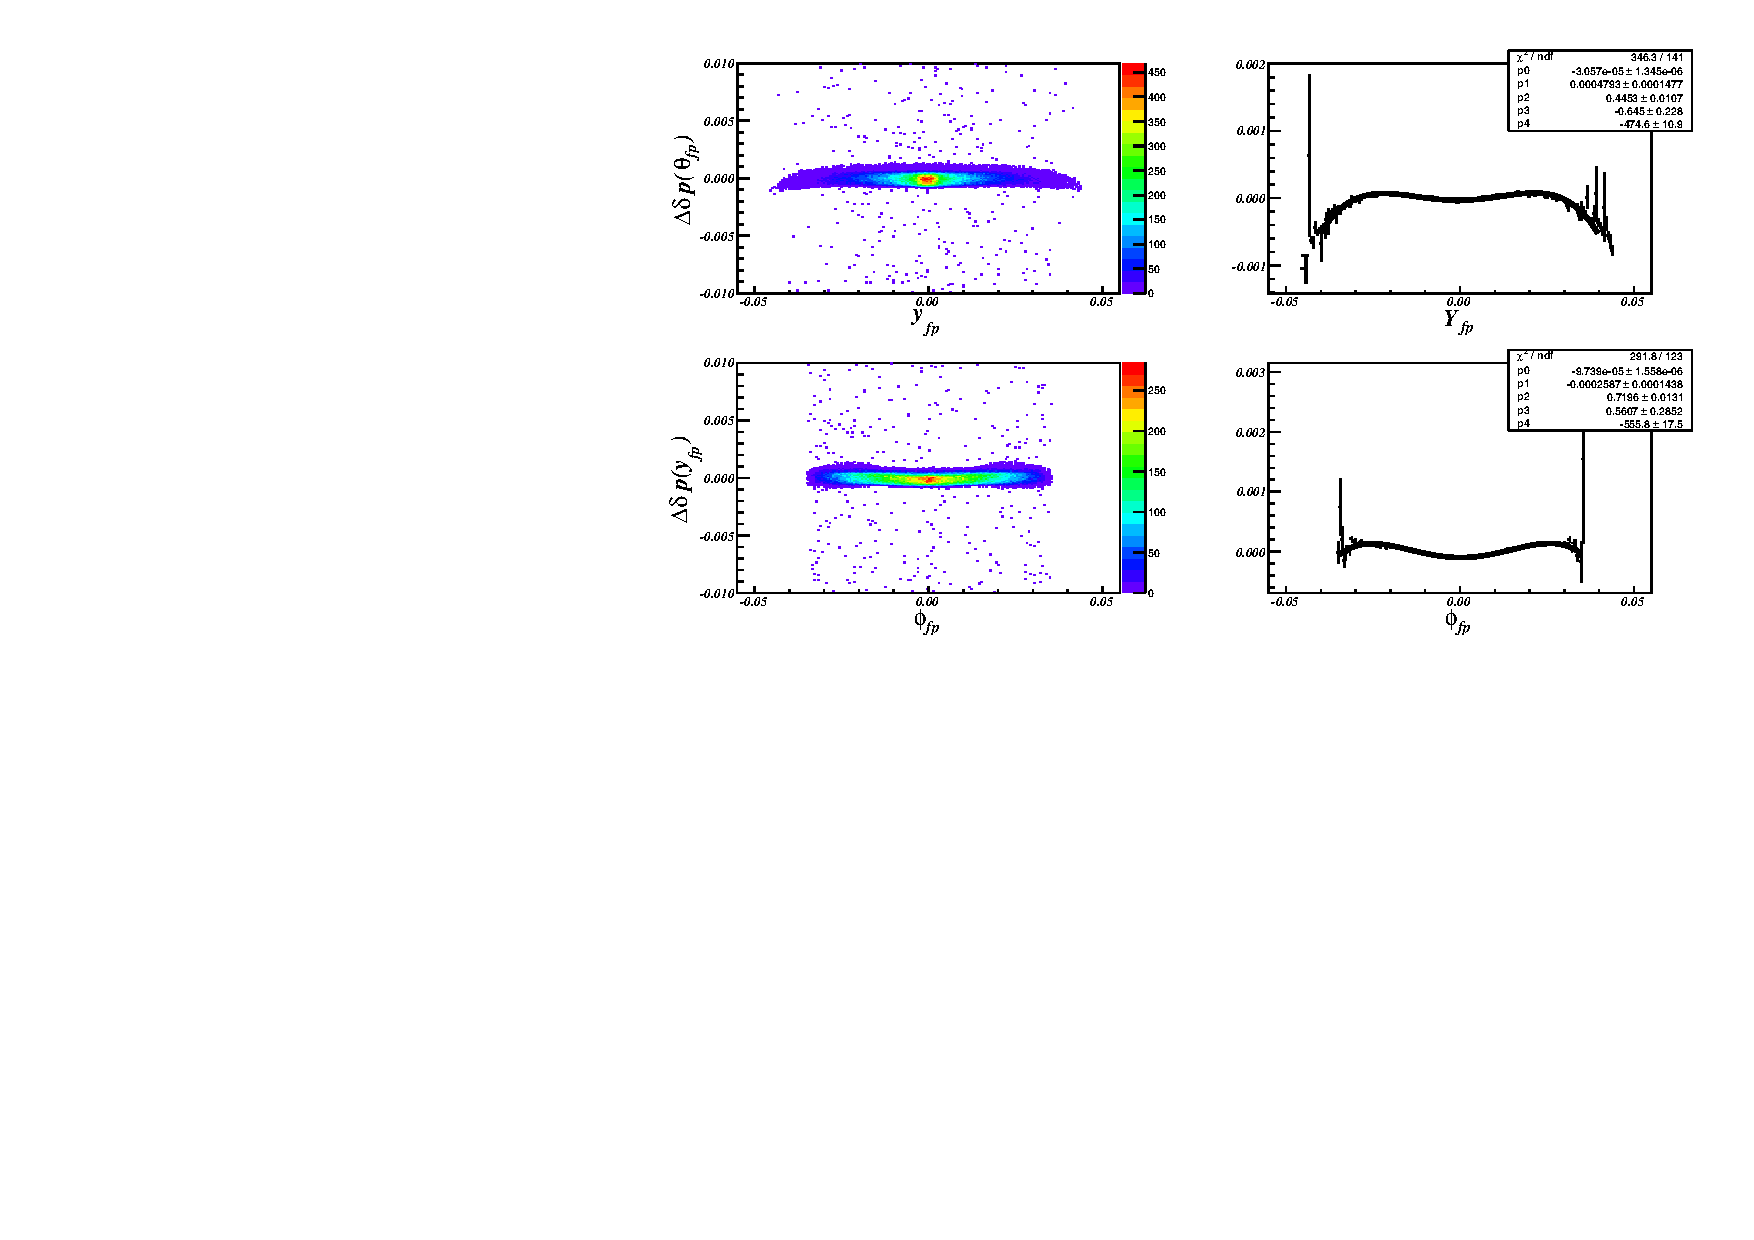
\includegraphics[type=pdf,ext=.pdf,read=.pdf,width=0.7\textwidth]{./figures/apend/DeltaCorr2_Kin31} 
    }
    \hfill
   \subfloat[$\Delta\delta p(\phi_{fp})$ .vs. $\delta p_{in}$]{
      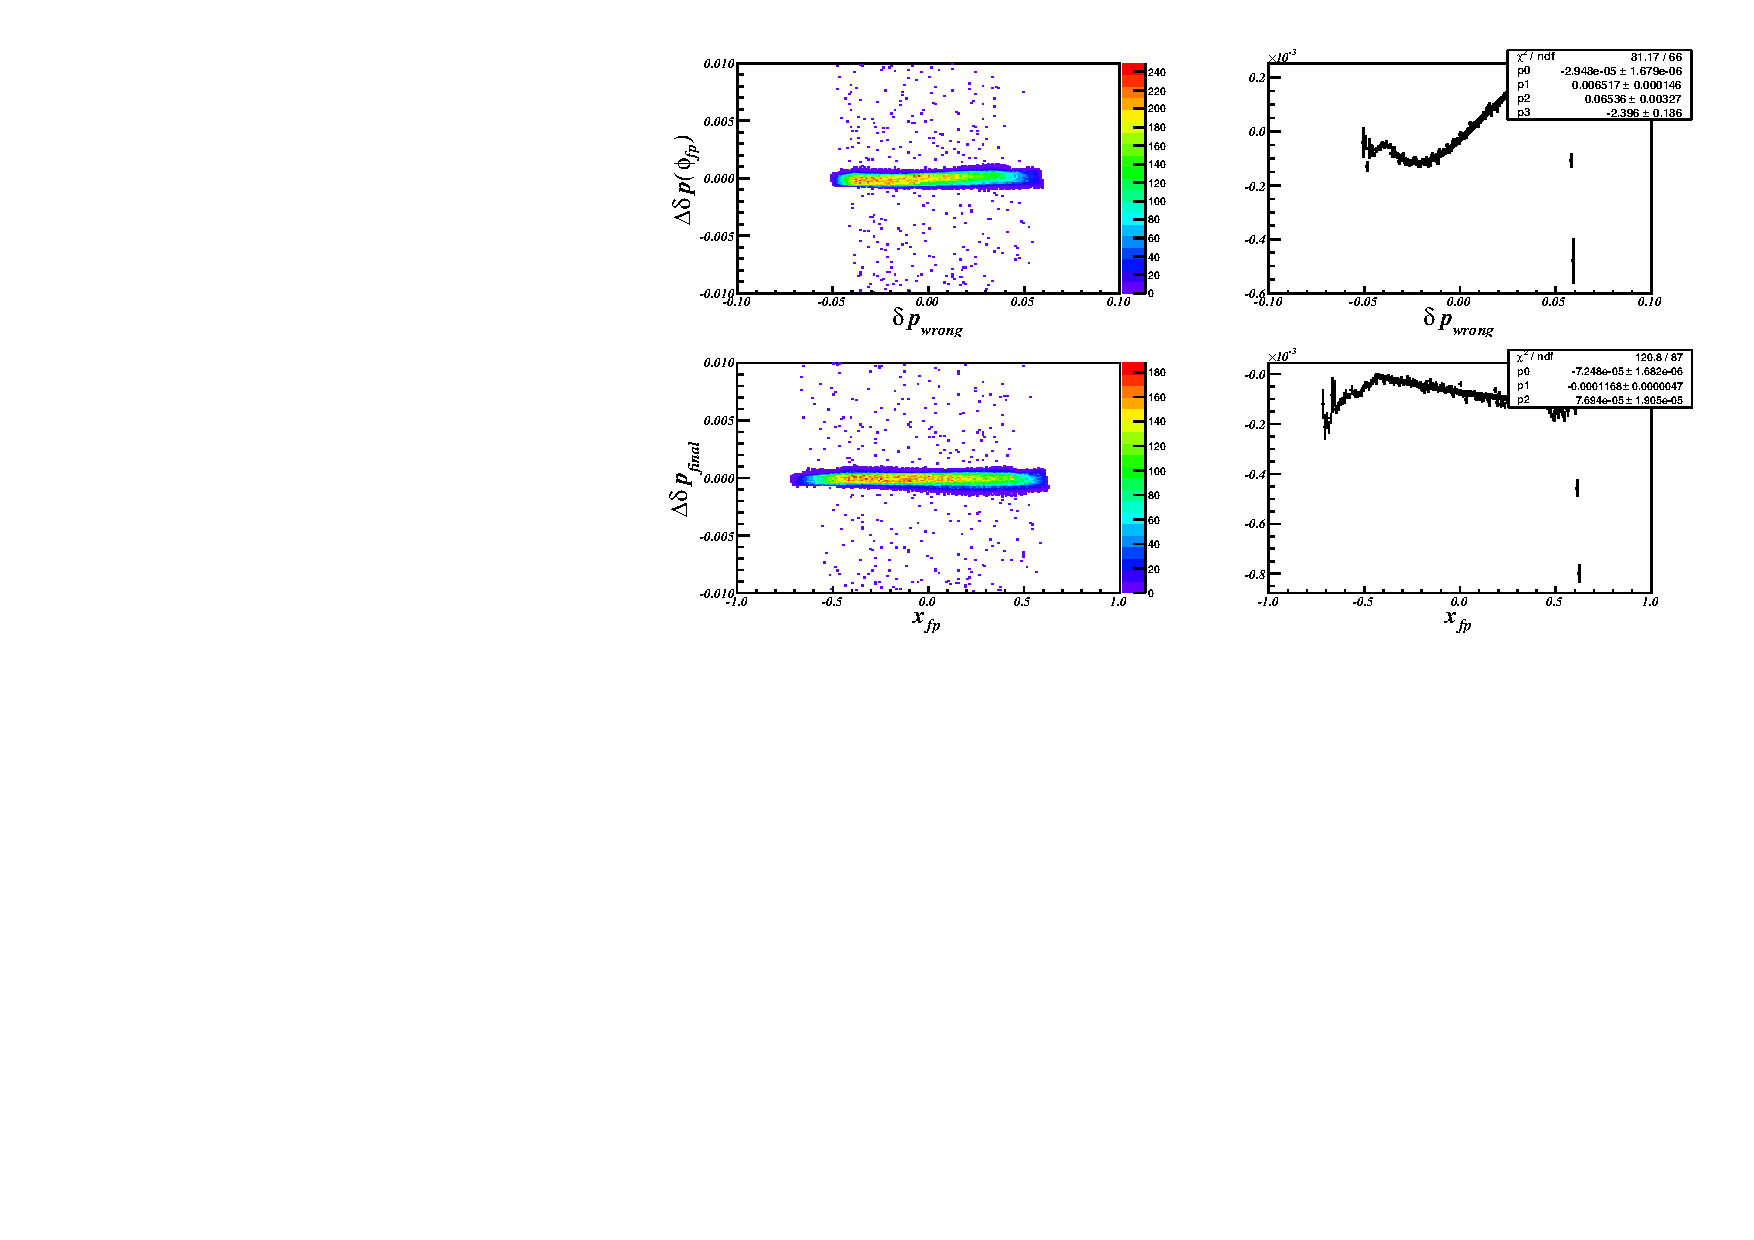
\includegraphics[type=pdf,ext=.pdf,read=.pdf,width=0.7\textwidth]{./figures/apend/DeltaCorr3_Kin31}
    }
    
    \caption[$\delta p$ correction function fitting]{\footnotesize{$\delta p$ correction function fitting with the focal plane variables. In each raw, the left is the 2-D histogram of $\Delta\delta p$ versus each fitting variable, while the right plot is the profile of the 2-D histogram, which is fitted with the polynomial function defined in Eq.~\eqref{deltap_corr_all}. The bottom two plots give the final result after applying all corrections.}}
    \label{deltap_fitting}
  \end{center}
\end{figure}

 Combining equations from Eq.~\eqref{deltap_corr_xfp} to Eq.~\eqref{deltap_corr_deltap}, Eq.~\eqref{dp_corr_func} leads to:
\begin{equation}
  \delta p_{cor}= \delta p_{in}+ f(x_{fp}, \theta_{fp}, y_{fp}, \phi_{fp}),
   \label{deltap_corr_all}
\end{equation}

 Fig.~\ref{deltap_fitting} shows the fitting result the distribution of $\Delta\delta p$ for each corrections. The final residual error, $\Delta\delta p(\delta p_{in})/\delta p_{cor}$, is close to $ 0.03\%$ (Fig.~\ref{deltap_final}) indicating that the mis-reconstructed momentum in the RQ3 has been corrected.
\begin{figure}[!ht]
 \begin{center}
  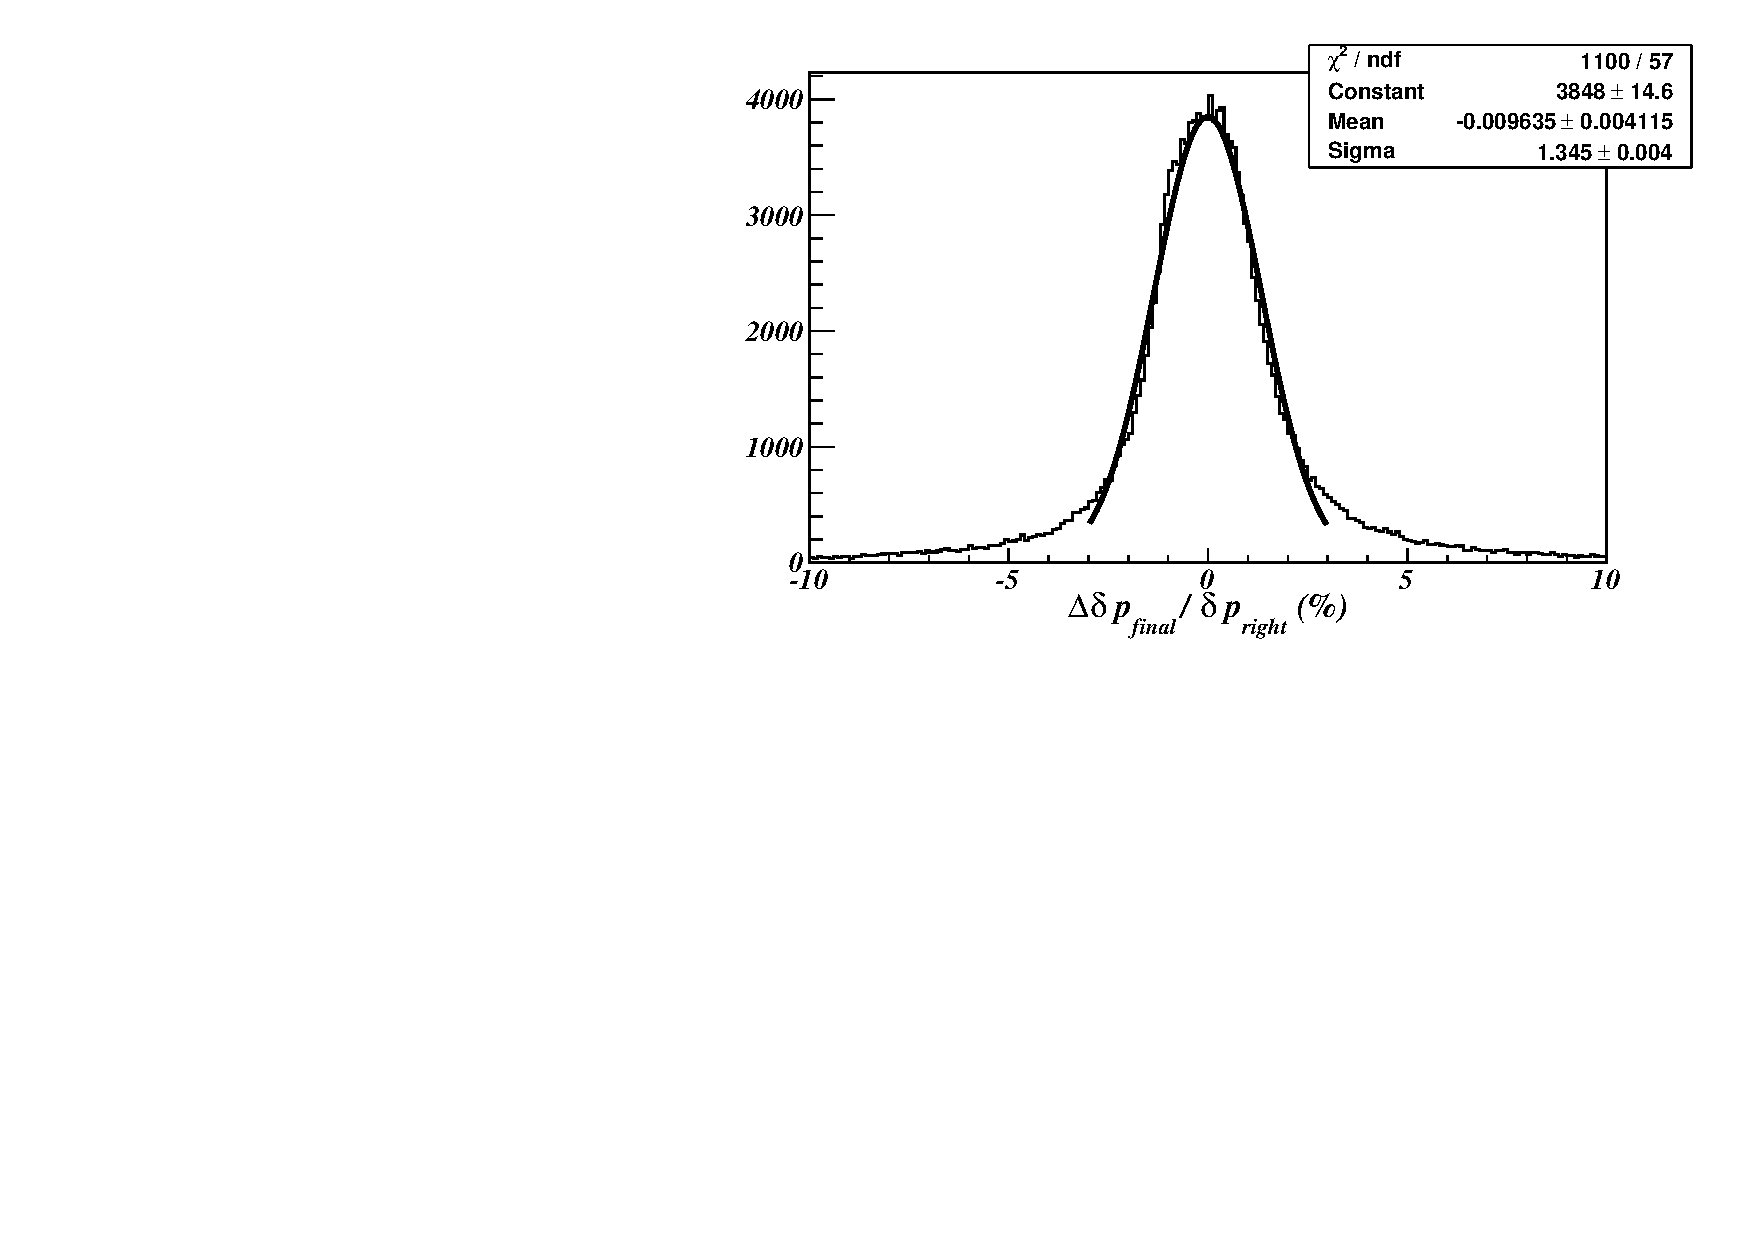
\includegraphics[type=pdf, ext=.pdf,read=.pdf,width=0.7\textwidth]{./figures/apend/DeltaCorr4_Kin31}
  \caption[The residual error of $\delta p$ correction function]{The residual error of $\delta p$ correction function. The momentum reconstruction value can be corrected with the error around $1.3\%$.}
  \label{deltap_final}
 \end{center}
\end{figure}
 \begin{figure}[!ht]
 \begin{center}
  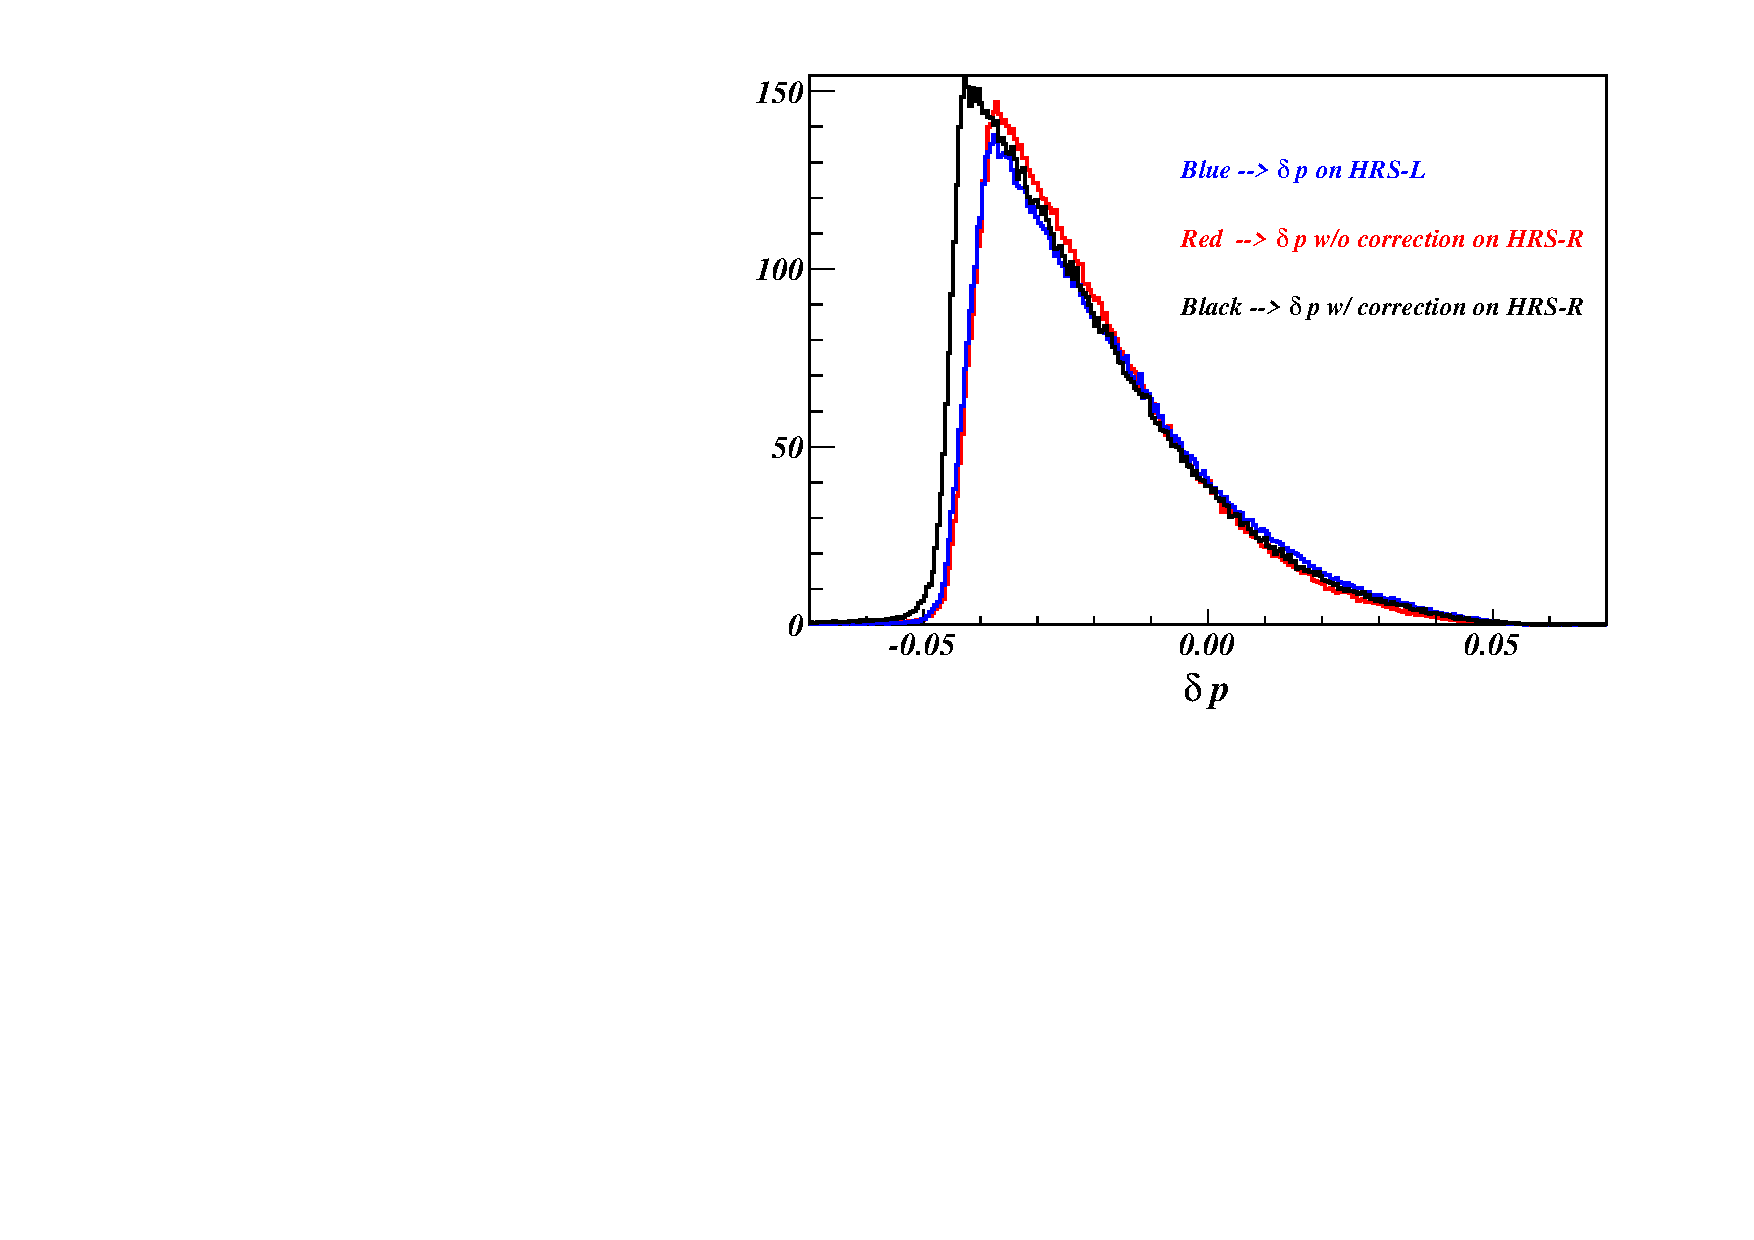
\includegraphics[type=pdf, ext=.pdf,read=.pdf,width=1.0\textwidth]{./figures/apend/DeltaP_Corr}
  \caption[$\delta p$ correction function applying on real data]{$\delta p$ correction function applying on real data. The data was taken on the carbon target with both HRSs at Kin5.0. The momentum distribution on HRS-R without the correction is different from the one on HRS-L (blue), which, however, agrees with the momentum distribution on HRS-R after the correction (black) at the central region. The $\delta p$ acceptance range on HRS-R is wider than the one on HRS-L, which can be explained by the defusing effect of the RQ3.}
  \label{deltap_corr_real}
 \end{center}
\end{figure}

 Eq.~\ref{deltap_corr_all} can be applied to the experimental data to correct the value of $\delta p$ for each event which is firstly reconstructed by the un-calibrated D-Terms in the HRS-R optics matrix. The performance of the correction can be examined by comparing the momentum distribution of the data taken in two HRSs with the same setting. Shown in Fig.~\ref{deltap_corr_real}, the momentum distribution on HRS-R should be identical to the one on HRS-L after applying the correction function, but its acceptance would be slightly wider than the one on HRS-L because of the defocussing effect of the RQ3.
\chapter{Non-Uniform Cryogenic Targets}
  As discussed in Section 5.4.2, the cryogenic targets (cryo-target) used in the E08-014, $\mathrm{^{2}H}$, $\mathrm{^{3}He}$ and $\mathrm{^{4}He}$, presented strange distributions in $z_{react}$. These distributions indicate that their densities were not uniform but instead, vary along the 20~cm cells. As proved by a Monte Carlo simulation of the cryogenic target system~\cite{silviu_target},  such non-uniform density profiles were caused by the poor design of the target cells and the direction of the cryogenic flow, as shown in Fig.~\ref{silviu_plots}.
\begin{figure}[!ht]
  \begin{center}
    \subfloat[$\mathrm{^{2}H}$]{
      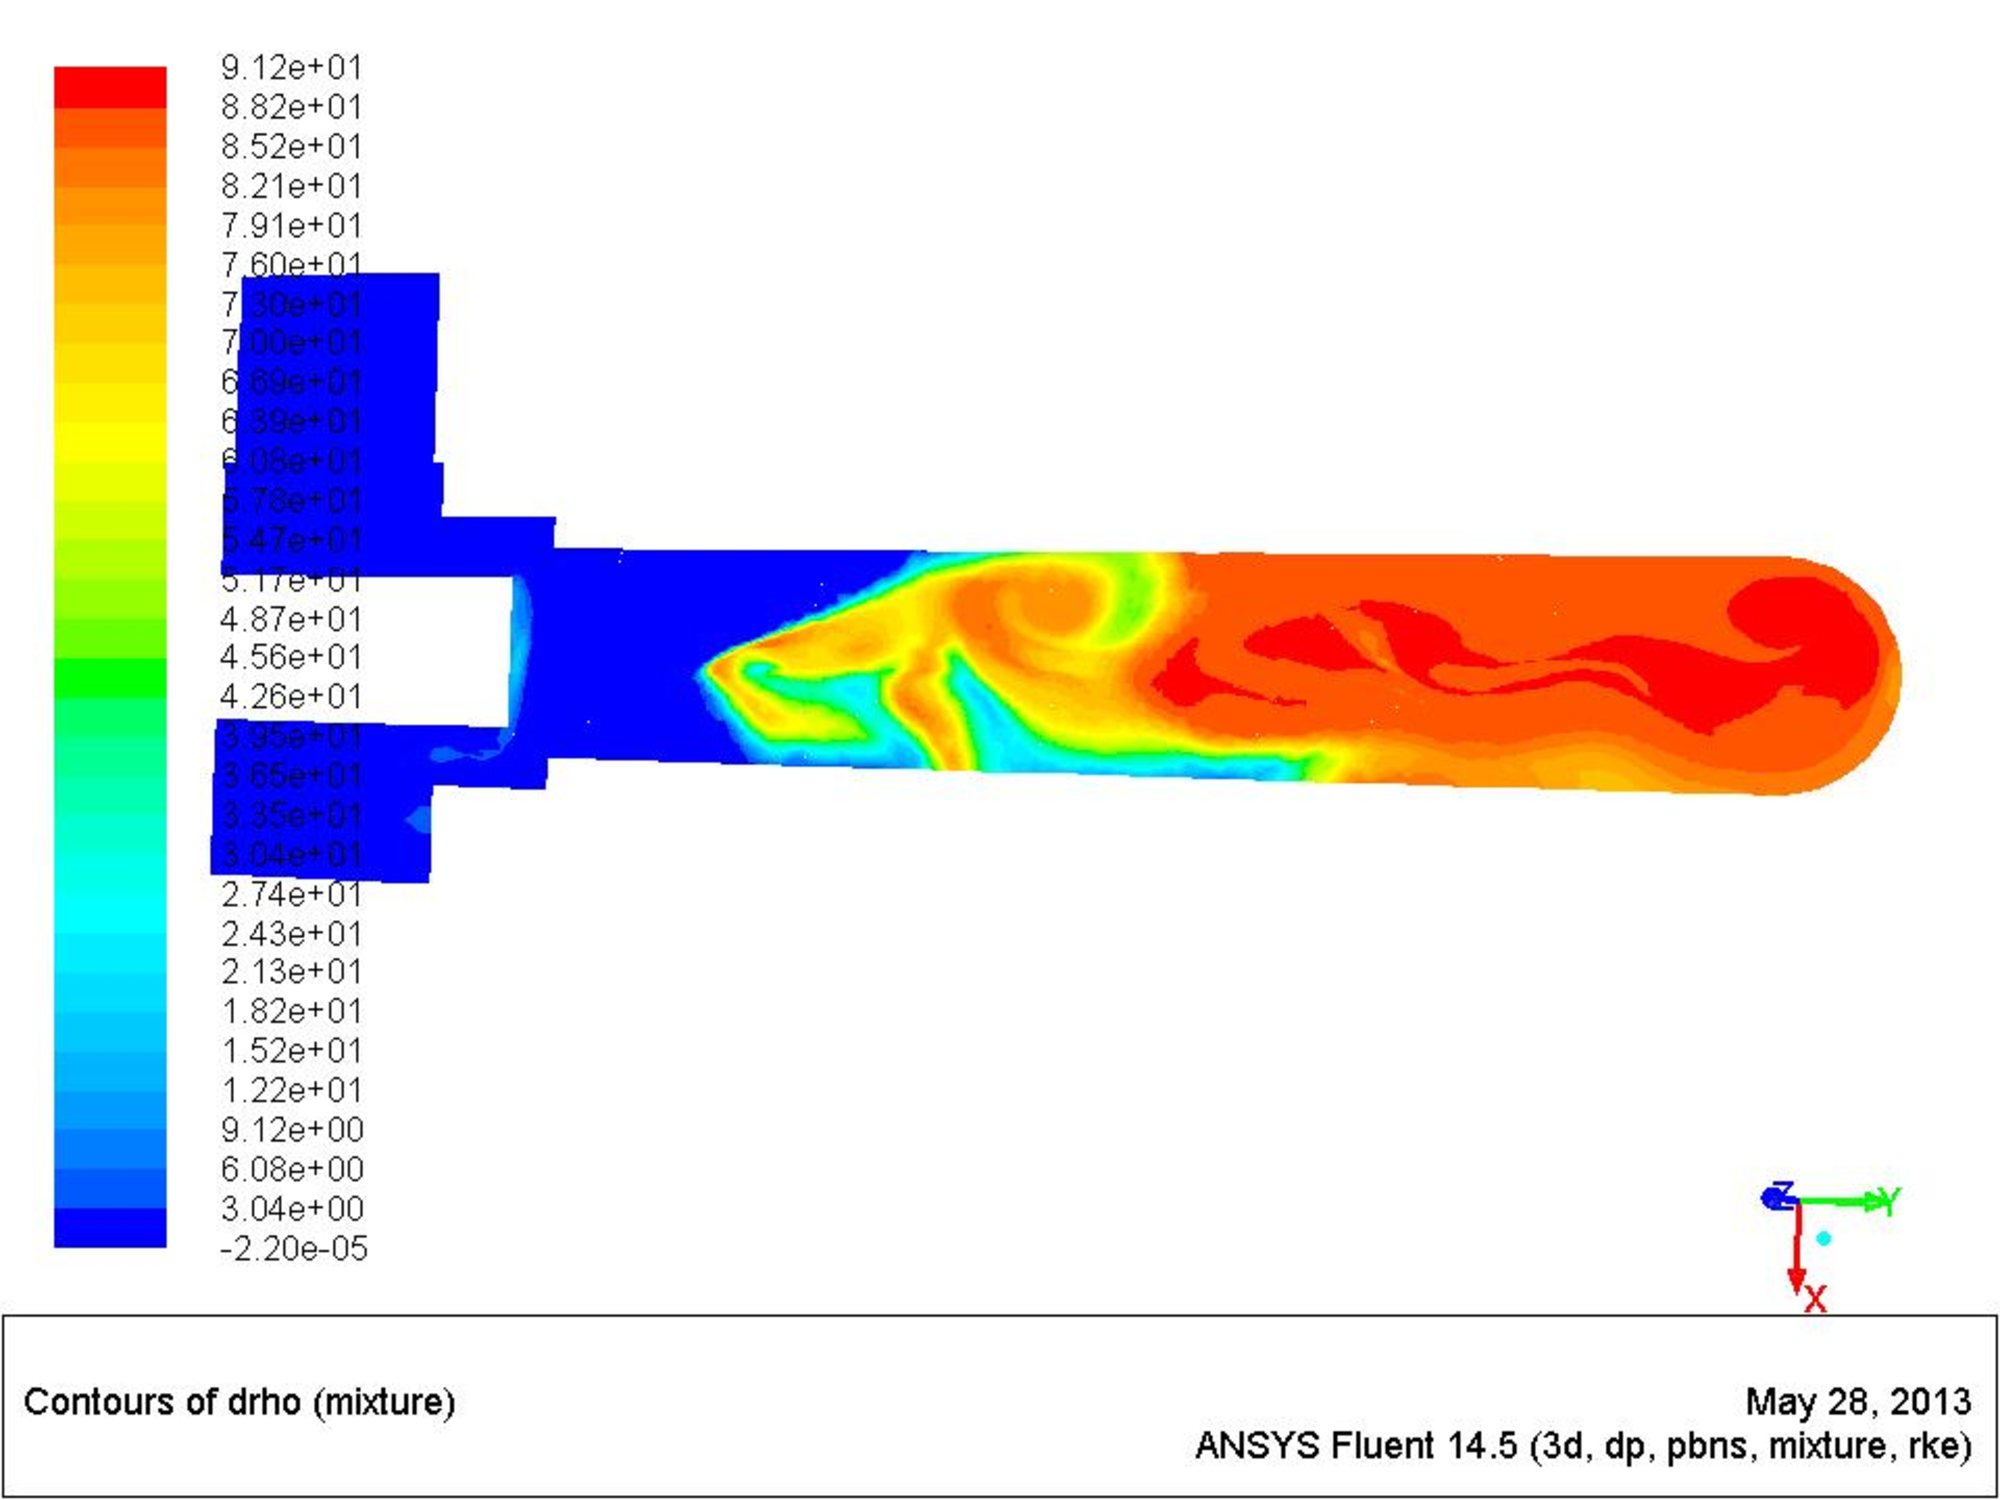
\includegraphics[type=pdf,ext=.pdf,read=.pdf,width=0.45\textwidth]{./figures/target/LD2_density} 
    }
    \hfill
     \subfloat[$\mathrm{^{4}He}$]{
      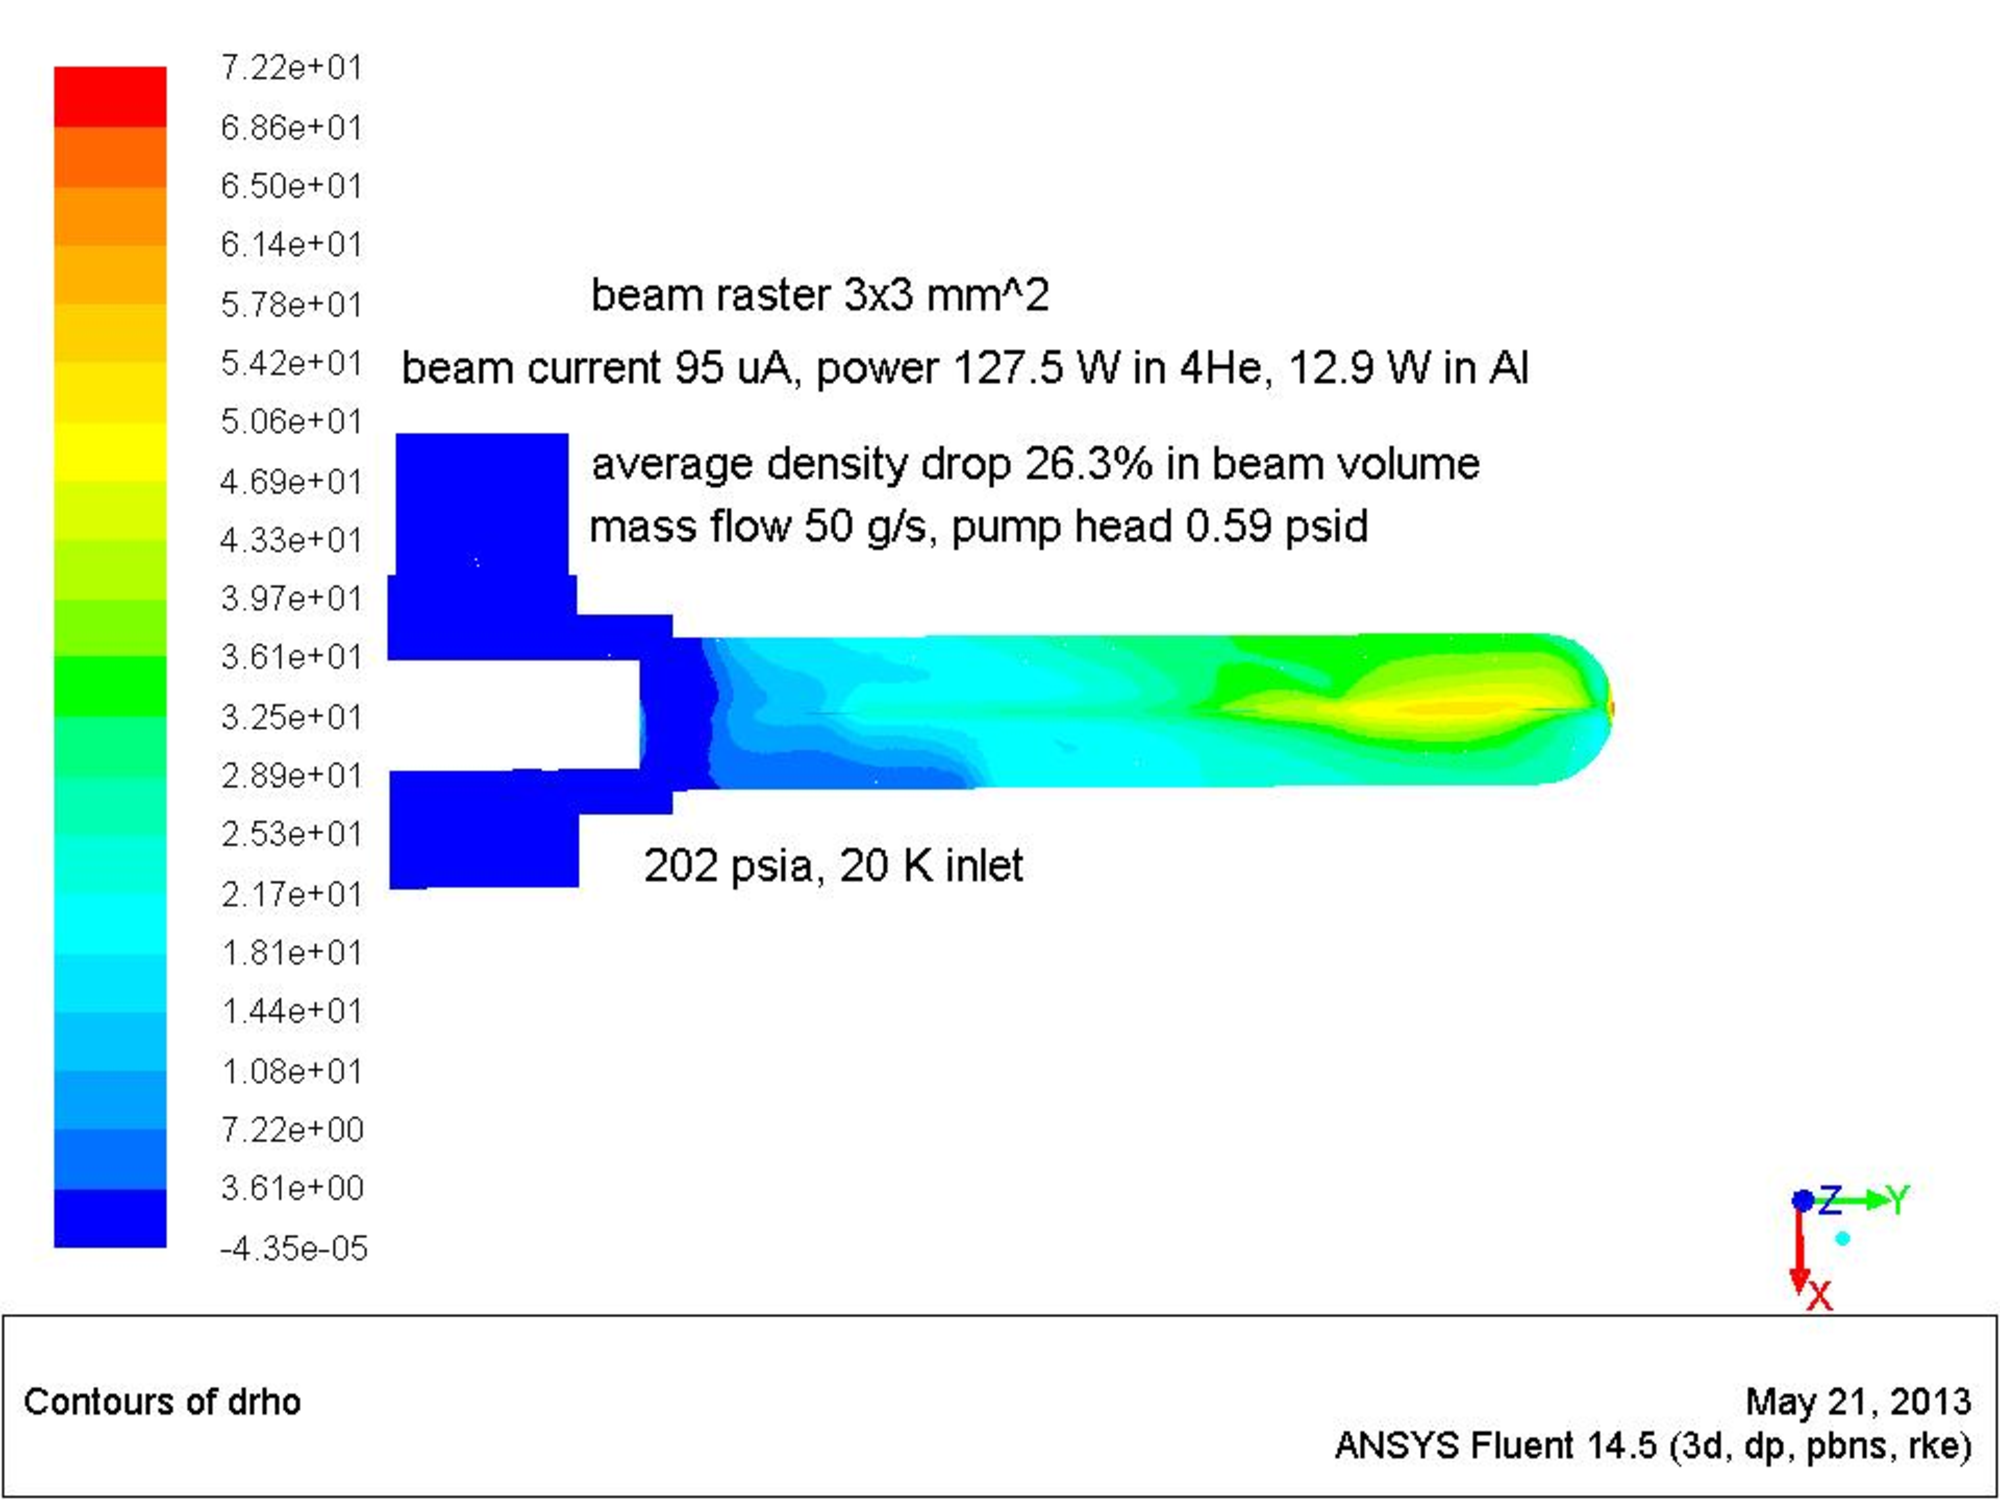
\includegraphics[type=pdf,ext=.pdf,read=.pdf,width=0.45\textwidth]{./figures/target/He4_density} 
    }
    \caption[Cryo-target density profiles from simulation]{\footnotesize{Cryo-target density profiles from simulation. The color contour denotes the value of the target density. The left plot is for $\mathrm{^{2}H}$ and the right plot is for $\mathrm{^{4}He}$. The density profile of $\mathrm{^{3}He}$ is not shown here. Both plots present the fluctuations of the target density along the cell.}}
    \label{silviu_plots}
  \end{center}
\end{figure}
 
  The absolute target density is required in order to extract the cross sections. The initial target density with the beam off can be determined before the experiment. When the beam is on, however, the density varies with the beam current because of the boiling effect. Such an effect is negligible for solid targets but it could be significant for cryo-targets. For a non-uniform cryo-target, the boiling effect differs along the target cell, and in addition, the radiation correction becomes more complicated since the radiation effect largely depends on the location and direction of the electron-scattering process. In this chapter, a detailed study of the boiling effect is given, followed by a discussion of extracting the cryo-target density distributions. A procedure to evaluate the radiation correction factors for non-uniform cryo-targets will be introduced in the end.

\section{Boiling Study}
 \begin{figure}[!ht]
  \begin{center}
    \subfloat[$\mathrm{^{12}C}$ on HRS-L]{
      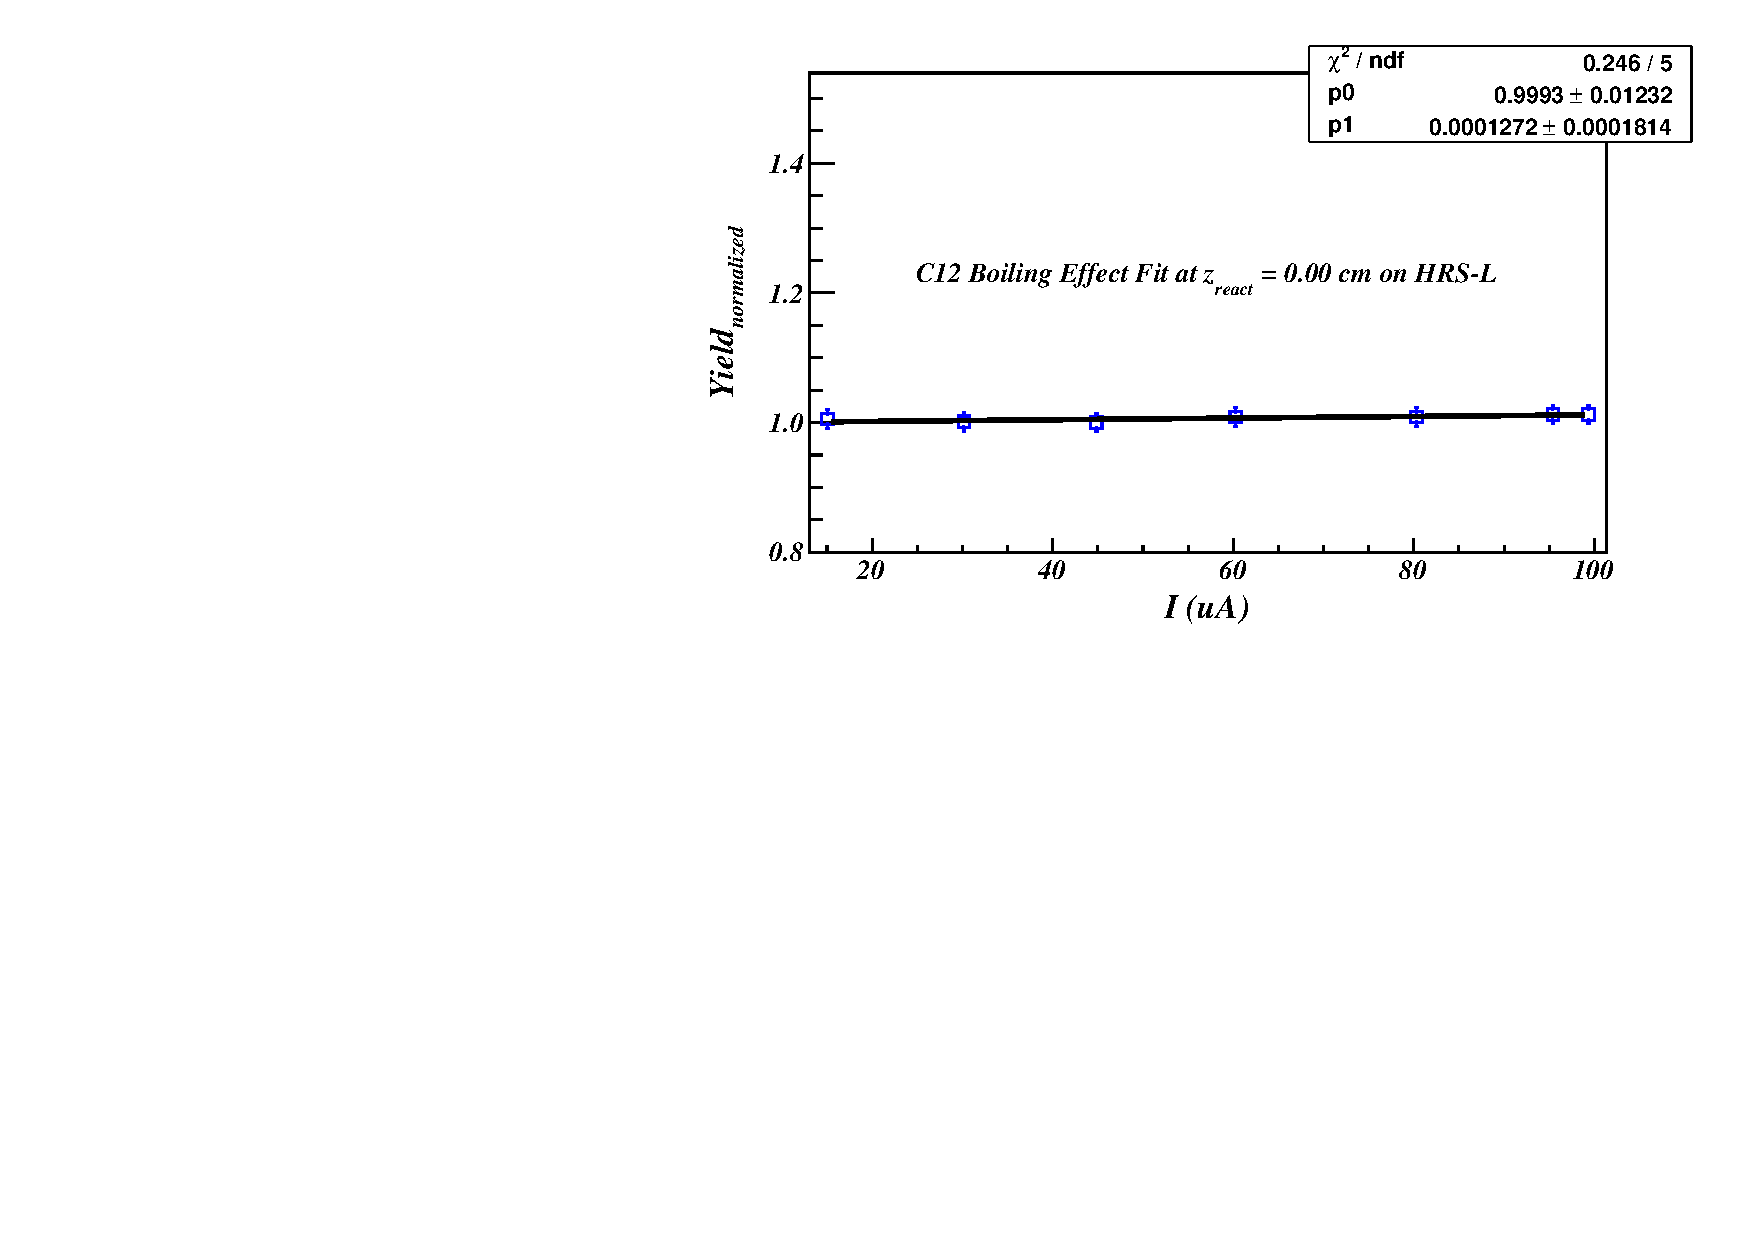
\includegraphics[type=pdf,ext=.pdf,read=.pdf,width=0.45\textwidth]{./figures/cryo/C12_Yield_L_All_0} 
    }
    \hfill
    \subfloat[$\mathrm{^{12}C}$ on HRS-R]{
      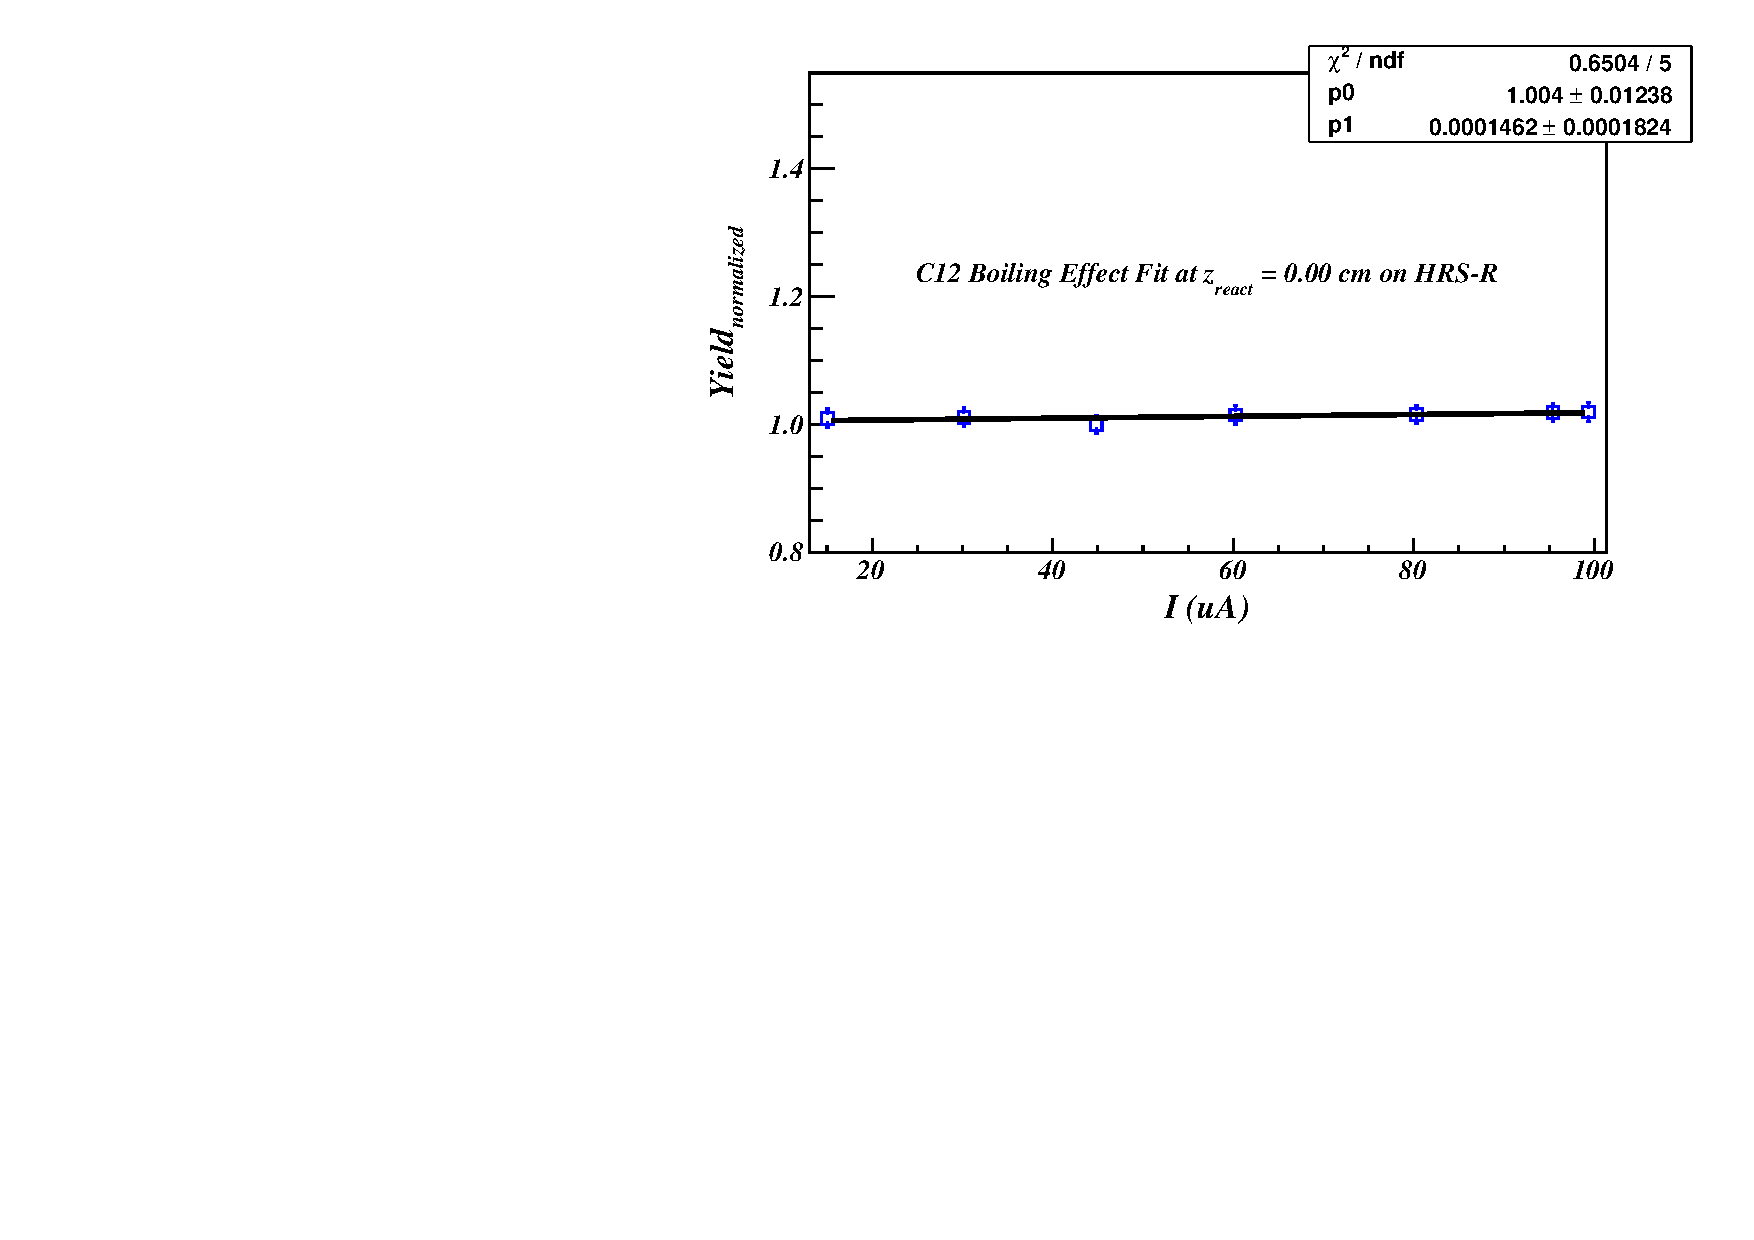
\includegraphics[type=pdf,ext=.pdf,read=.pdf,width=0.45\textwidth]{./figures/cryo/C12_Yield_R_All_0} 
    }
    \caption[$\mathrm{^{12}C}$ boiling effect fitting]{\footnotesize{$\mathrm{^{12}C}$ boiling effect fitting. Since $\mathrm{^{12}C}$ should have very small boiling effect, this study is used to check any rate-dependence effect at different current settings. The yield values have been normalized by a common factor.}}
    \label{c12_boil_fit}
  \end{center}
\end{figure}
  During the E08-014, several boiling study runs were taken with different beam current on these cryo-targets, as well as on the $\mathrm{^{12}C}$ target which was used to check any rate-dependence effects.
  
  The experimental yield depends on the target density, the beam charge and the cross section of electron-nucleus scattering. While the average cross section shouldn't change for one kinematic setting, the yield normalized by the beam charge should be directly proportional to the target density:
\begin{equation}
  Y(I) = Y(0) + m\cdot I,
  \label{eq_yield_boiling}
\end{equation}  
where $Y(I)$, the yield for one run with the beam current $I$, is equal to the total number of experimental events after all necessary cuts divided by the the total accumulated charge. $Y(0)$ is the yield extrapolated to zero beam current and $m$ is the slop of $Y(I)$ on $I$. By fitting Eq.~\eqref{eq_yield_boiling} with the data of the boiling study runs, one can obtain the variation of the target density at different current, given as:
\begin{equation}
  \rho(I) = \rho(0) \cdot (1.0 + BF \cdot I /100),
  \label{eq_yield_rho}
\end{equation}
where $BF=Y(0)/m$ is the boiling factor of the target.

\begin{figure}[!h]
  \begin{center}
    \subfloat[$\mathrm{^{2}H}$ on HRS-L]{
      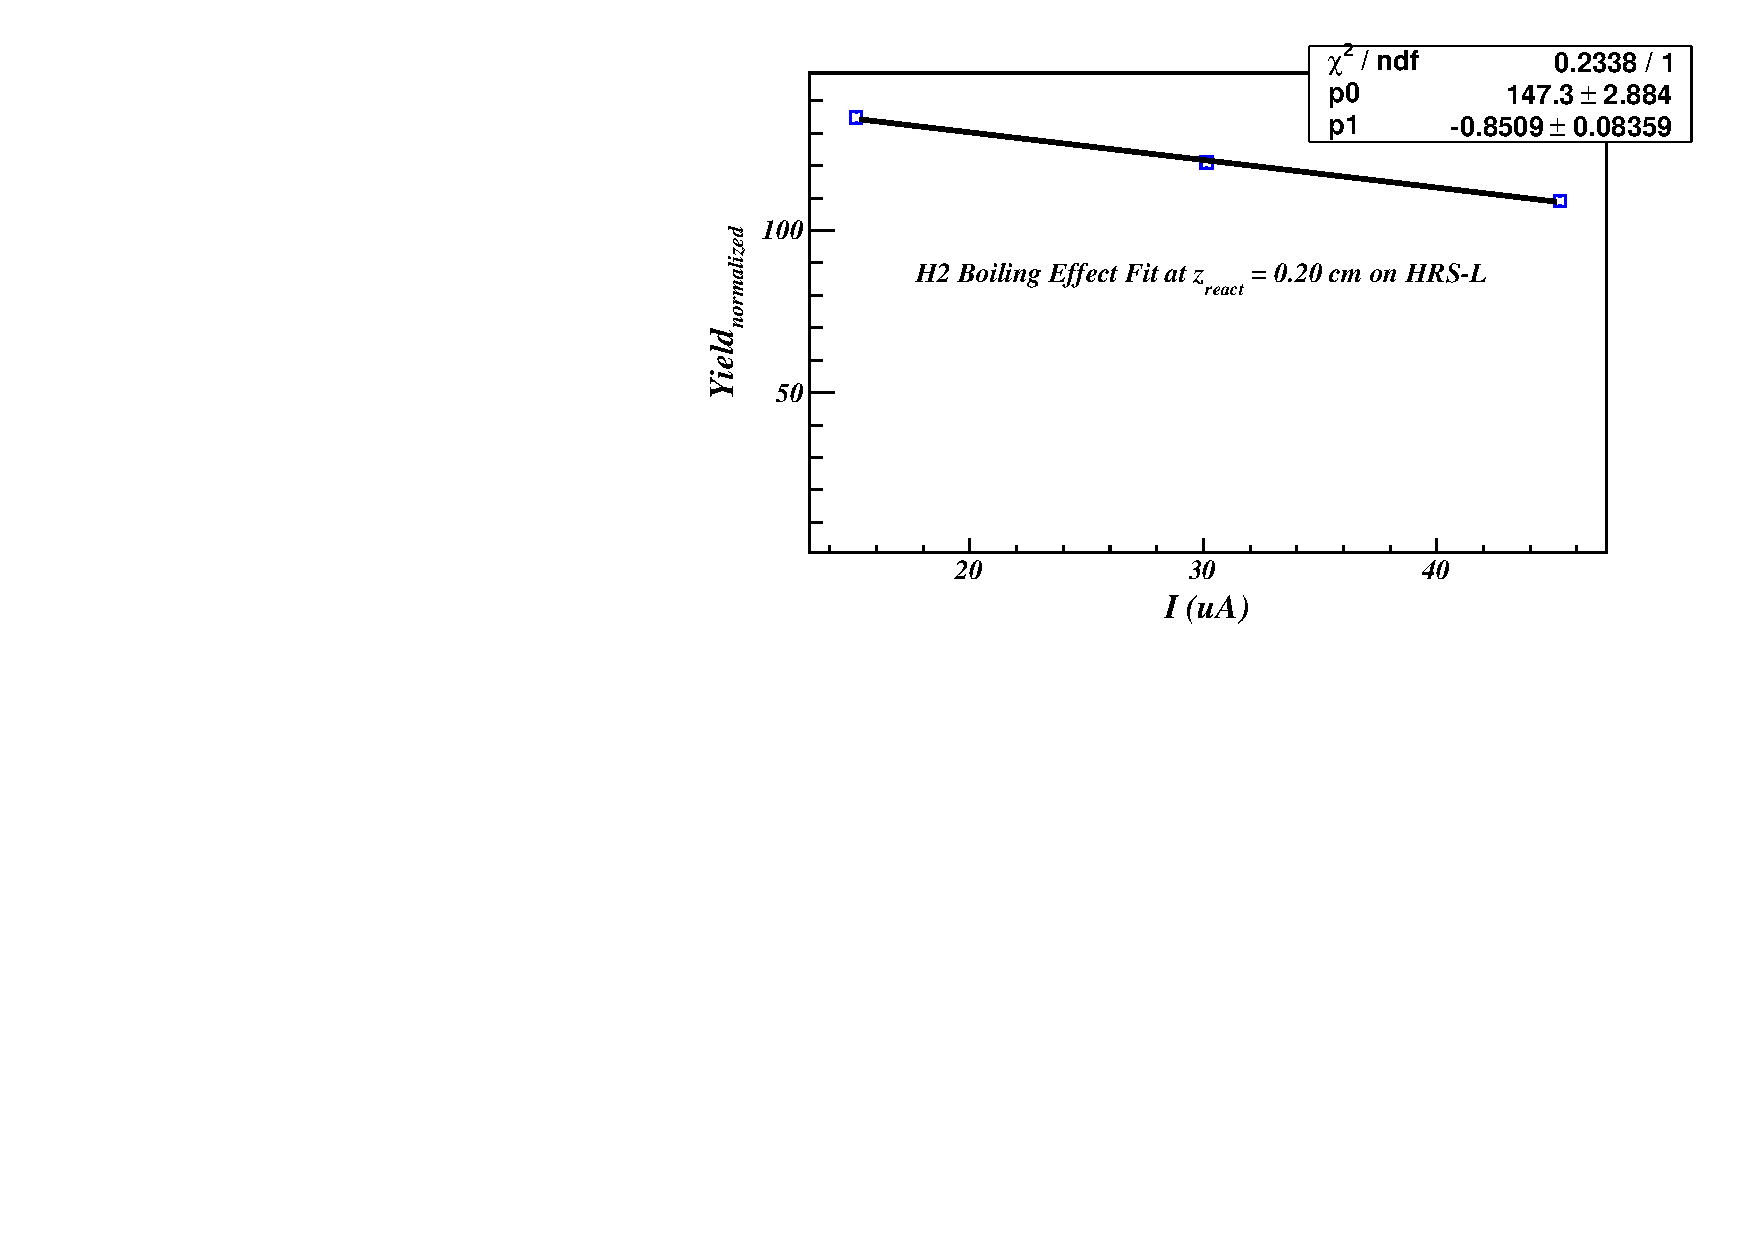
\includegraphics[type=pdf,ext=.pdf,read=.pdf,width=0.45\textwidth]{./figures/cryo/H2_Yield_L_All_0} 
    }
    \hfill
    \subfloat[$\mathrm{^{2}H}$ on HRS-R]{
      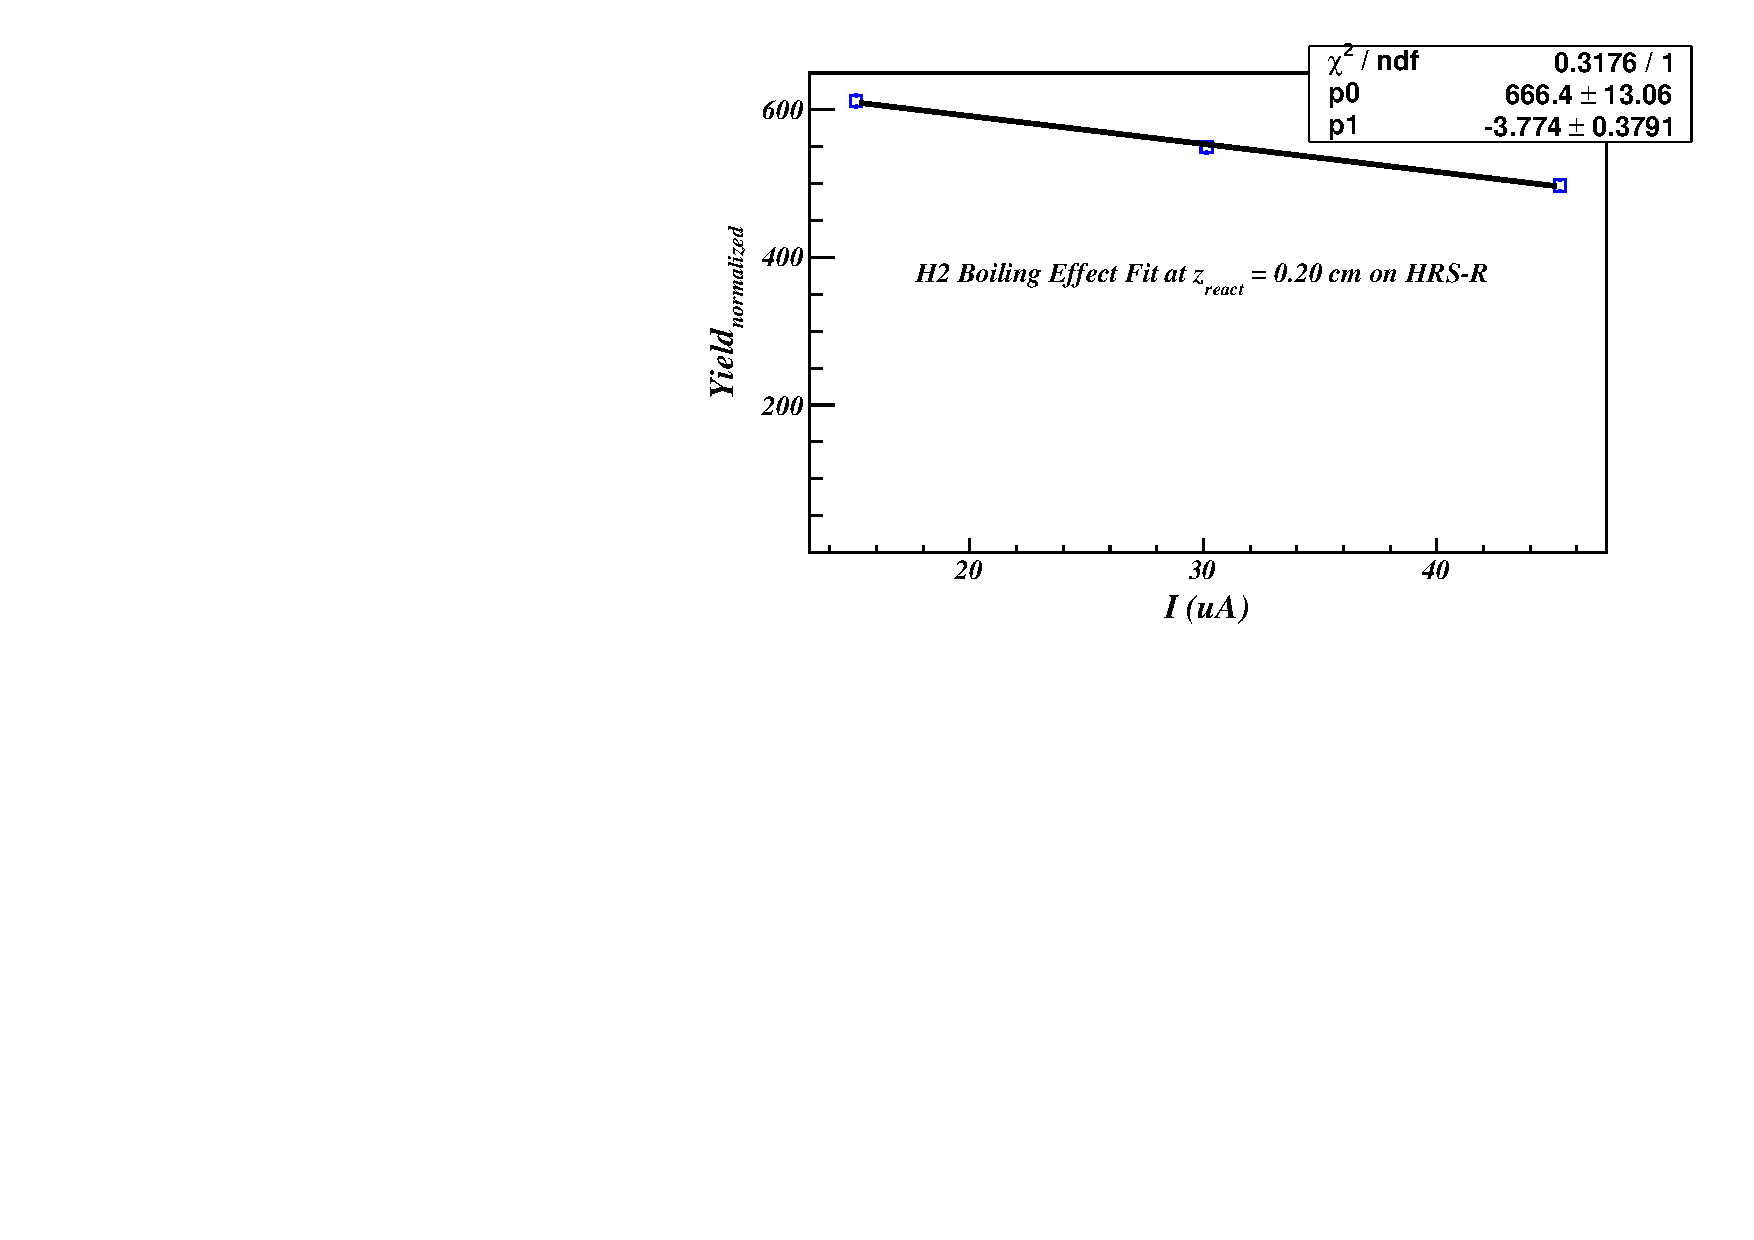
\includegraphics[type=pdf,ext=.pdf,read=.pdf,width=0.45\textwidth]{./figures/cryo/H2_Yield_R_All_0} 
    }
\\
    \subfloat[$\mathrm{^{3}He}$ on HRS-L]{
      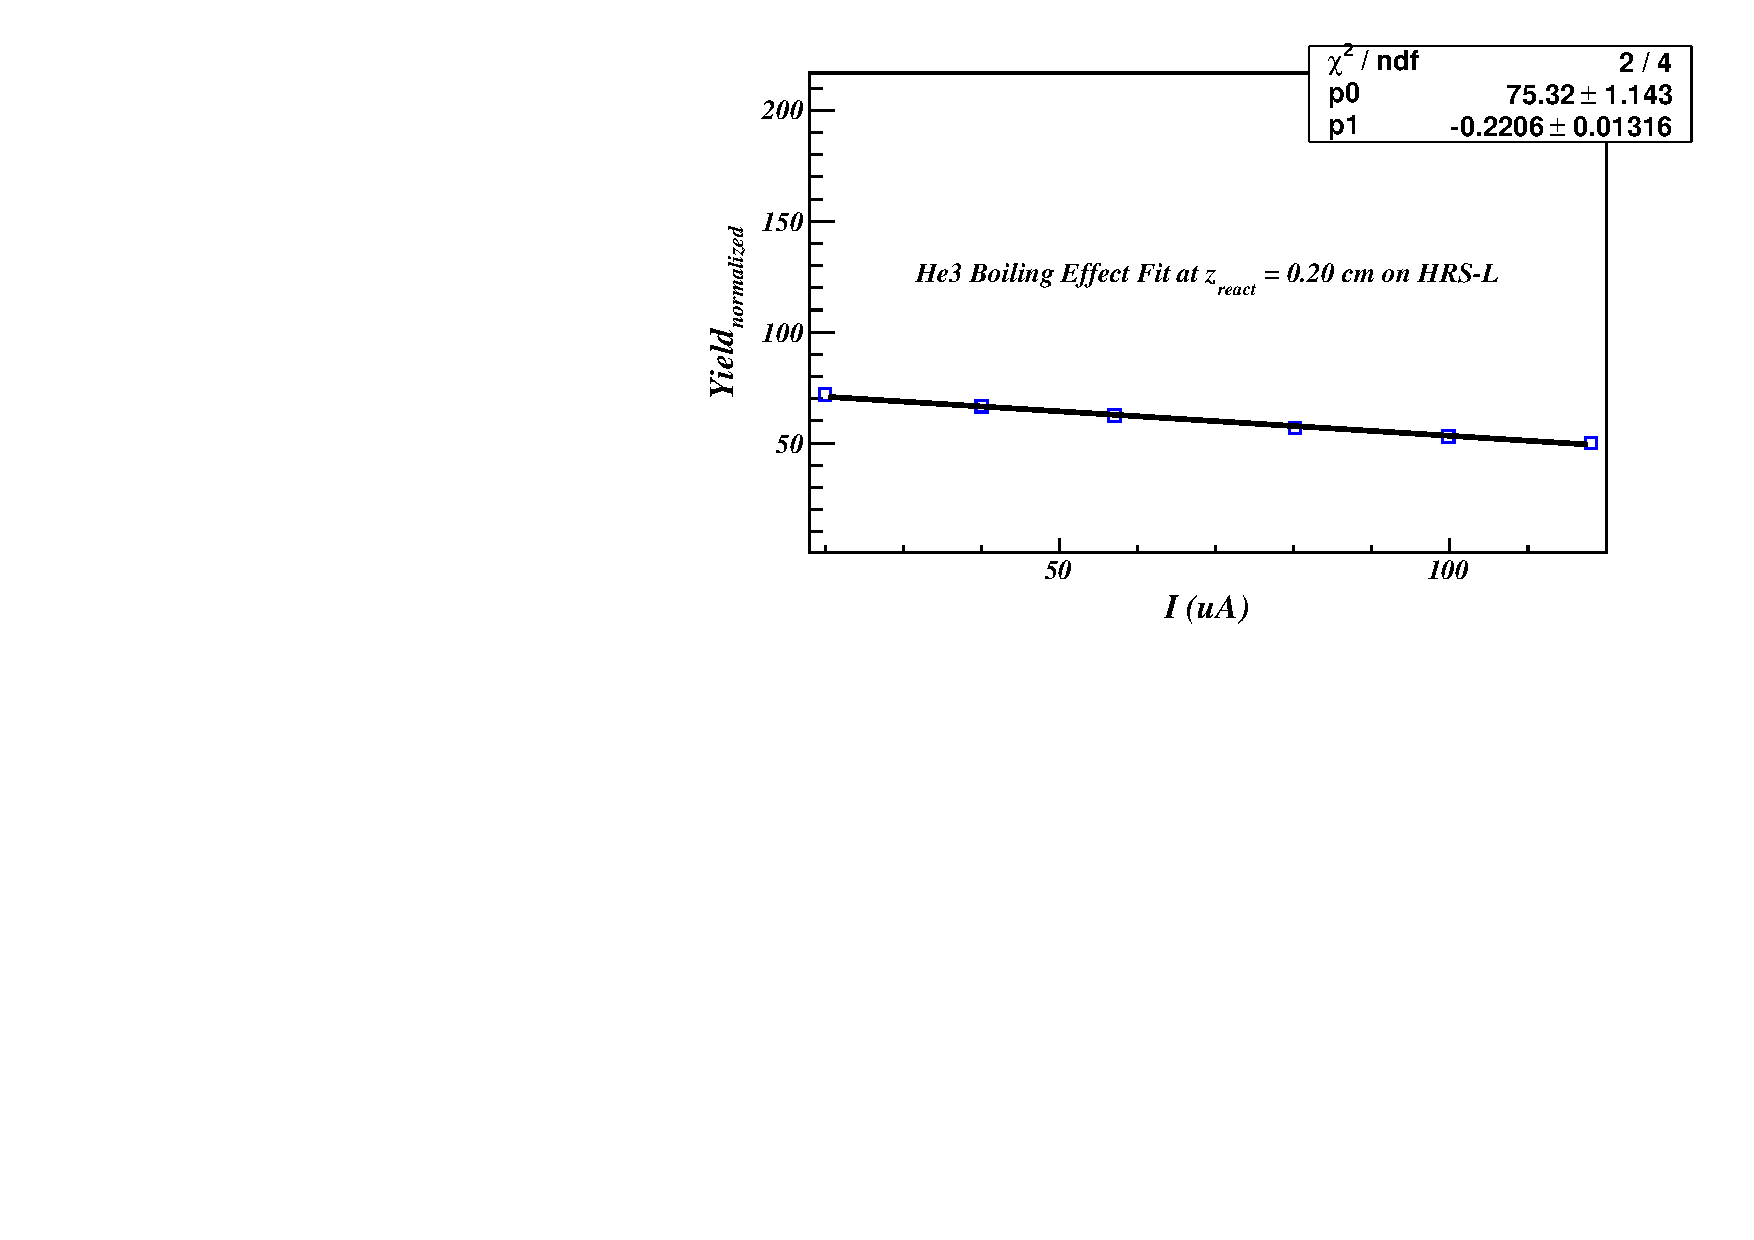
\includegraphics[type=pdf,ext=.pdf,read=.pdf,width=0.45\textwidth]{./figures/cryo/He3_Yield_L_All_0} 
    }
    \hfill
    \subfloat[$\mathrm{^{3}He}$ on HRS-R]{
      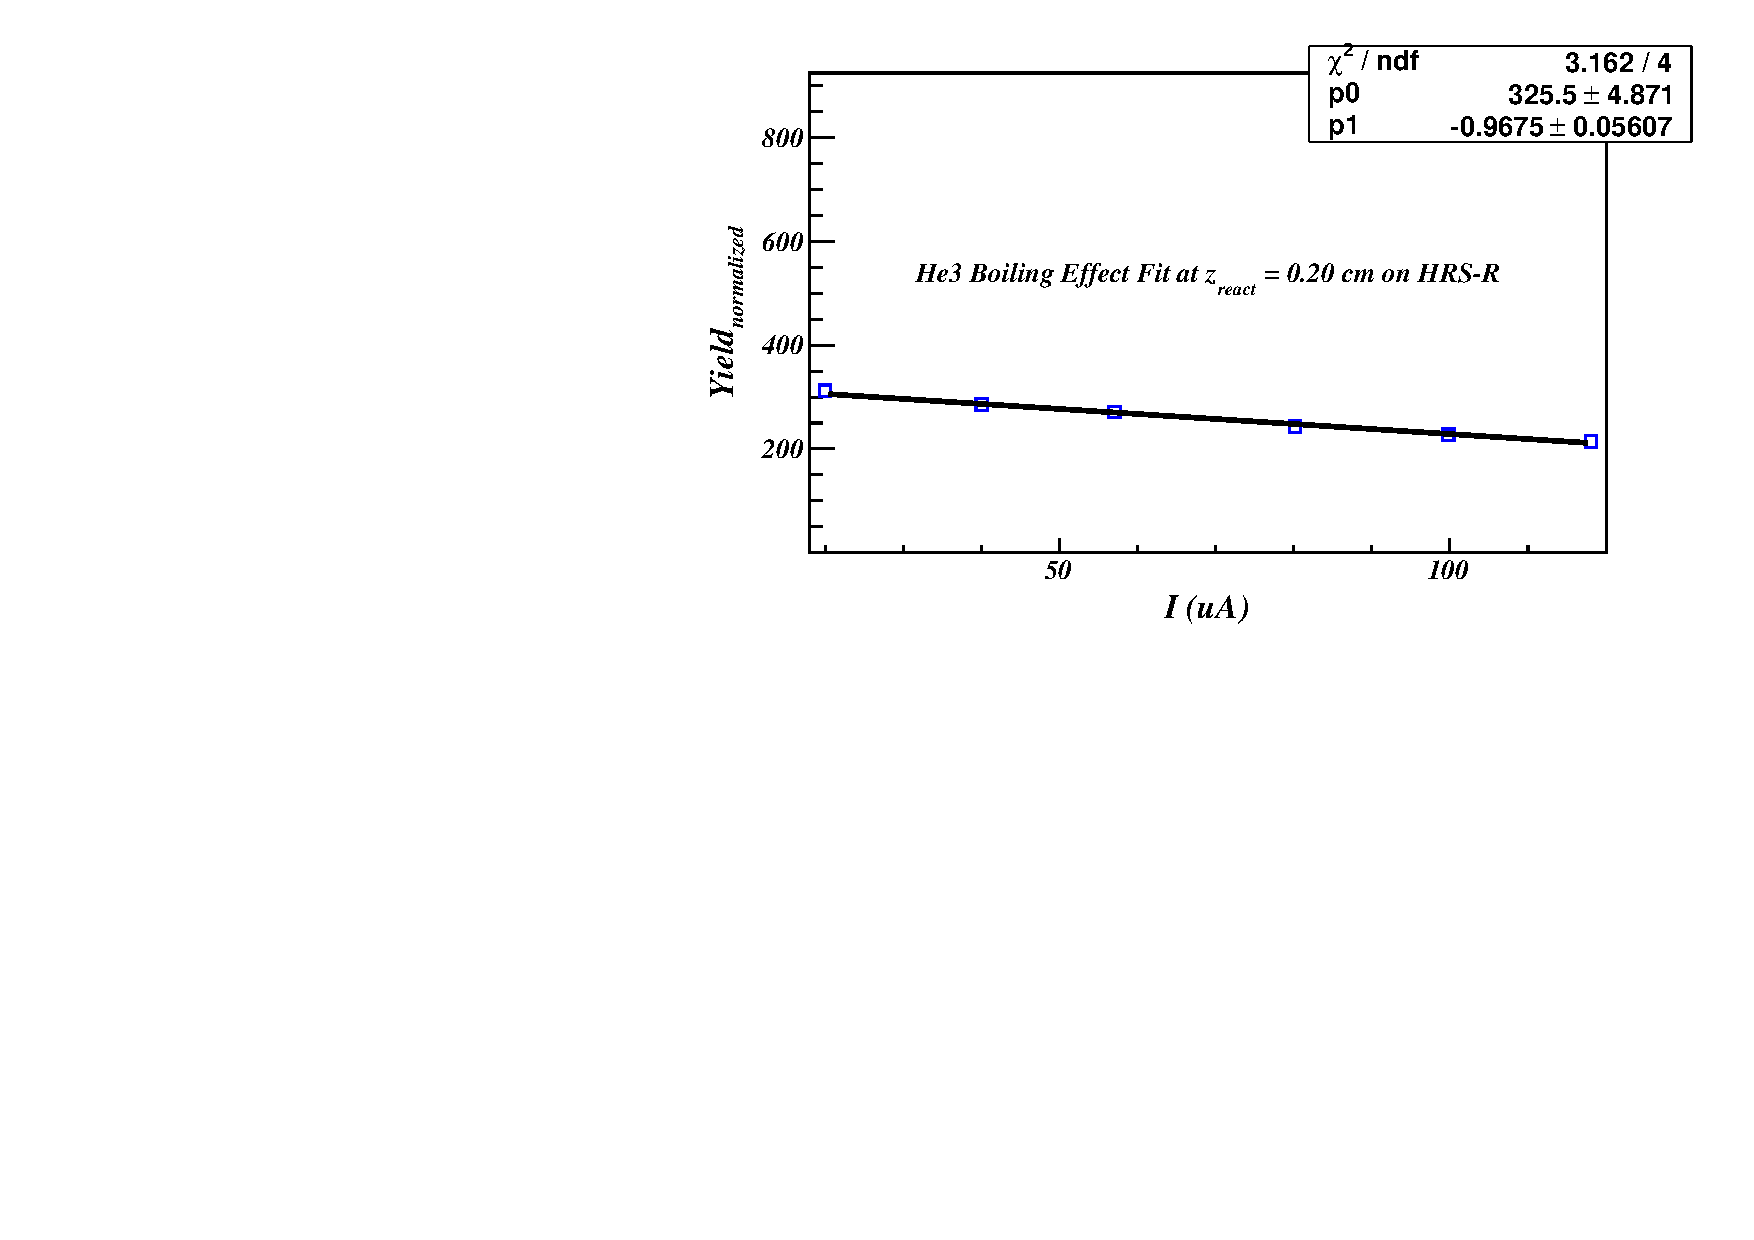
\includegraphics[type=pdf,ext=.pdf,read=.pdf,width=0.45\textwidth]{./figures/cryo/He3_Yield_R_All_0} 
    }
\\
    \subfloat[$\mathrm{^{4}He}$ on HRS-L]{
      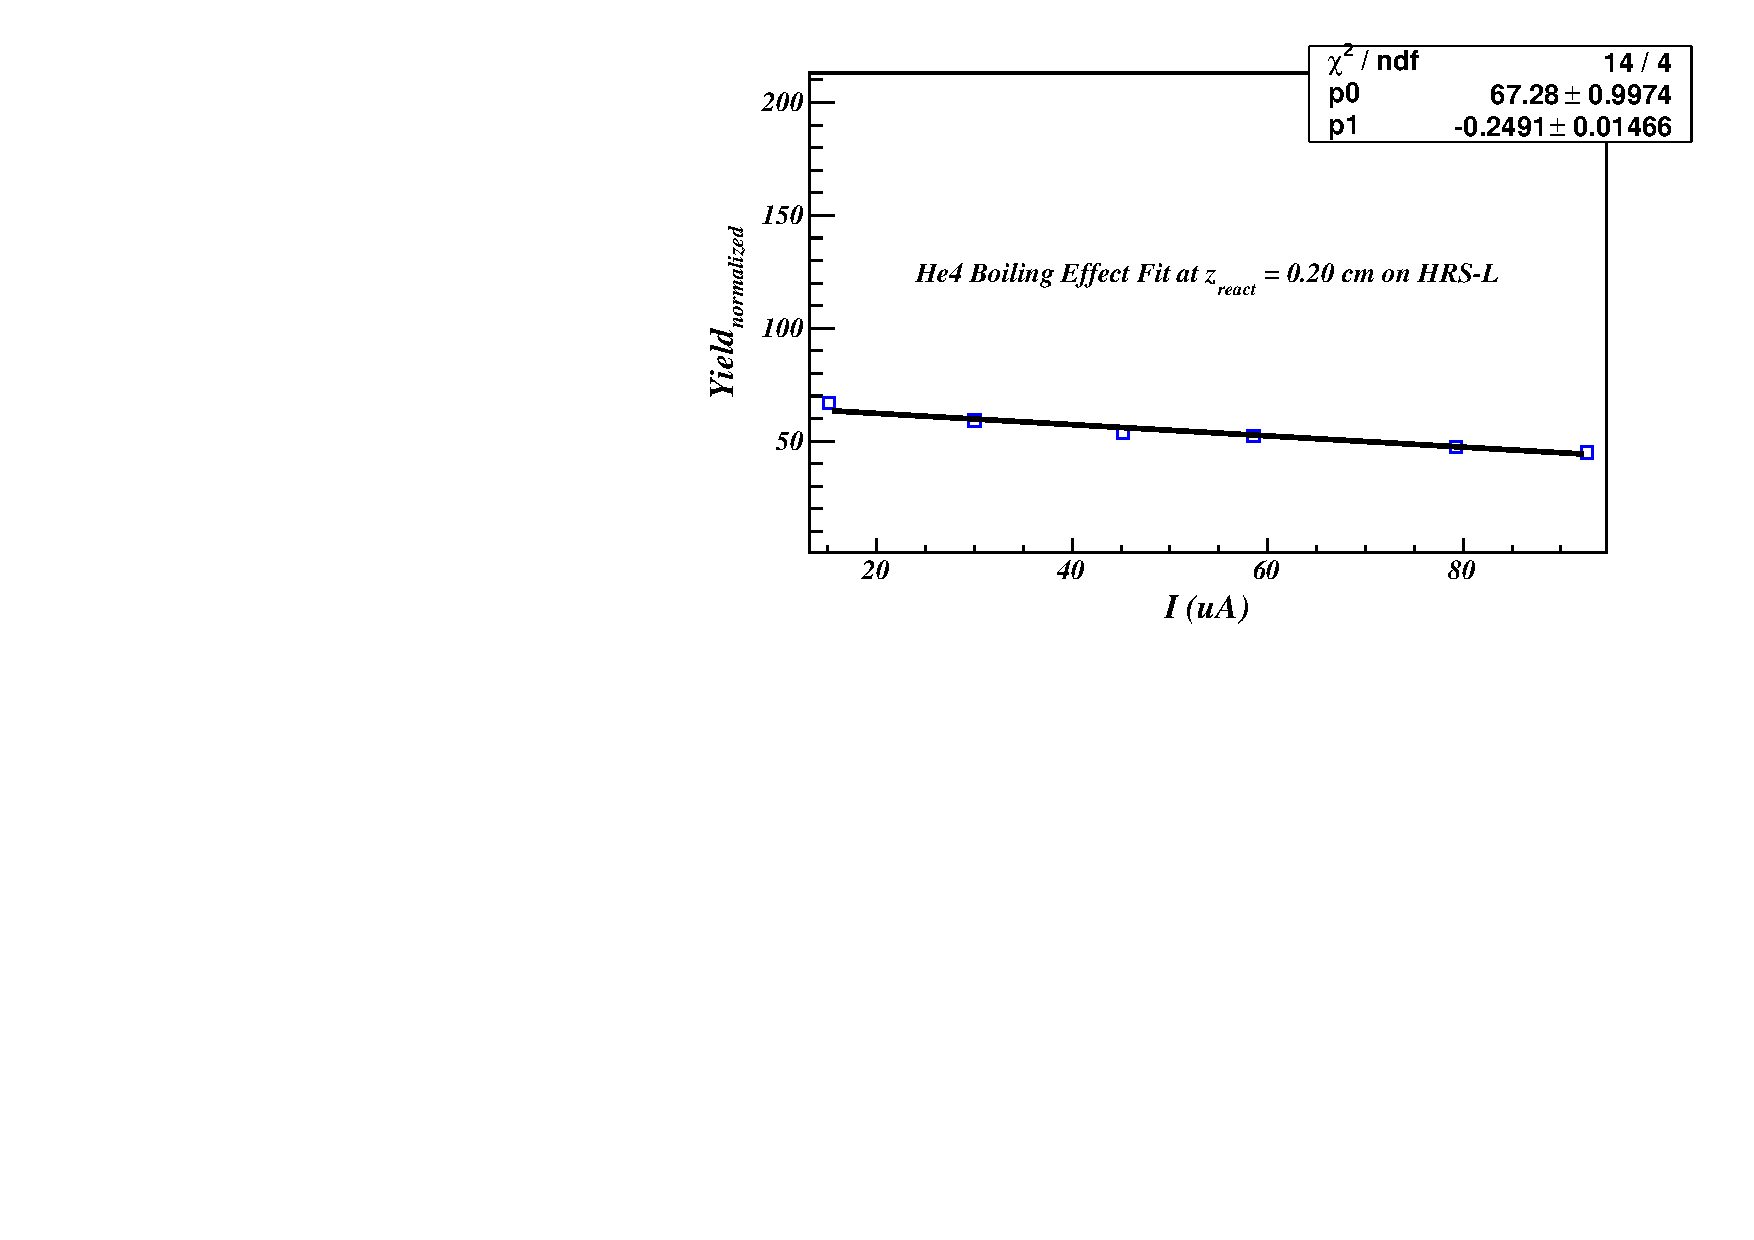
\includegraphics[type=pdf,ext=.pdf,read=.pdf,width=0.45\textwidth]{./figures/cryo/He4_Yield_L_All_0} 
    }
    \hfill
    \subfloat[$\mathrm{^{4}He}$ on HRS-R]{
      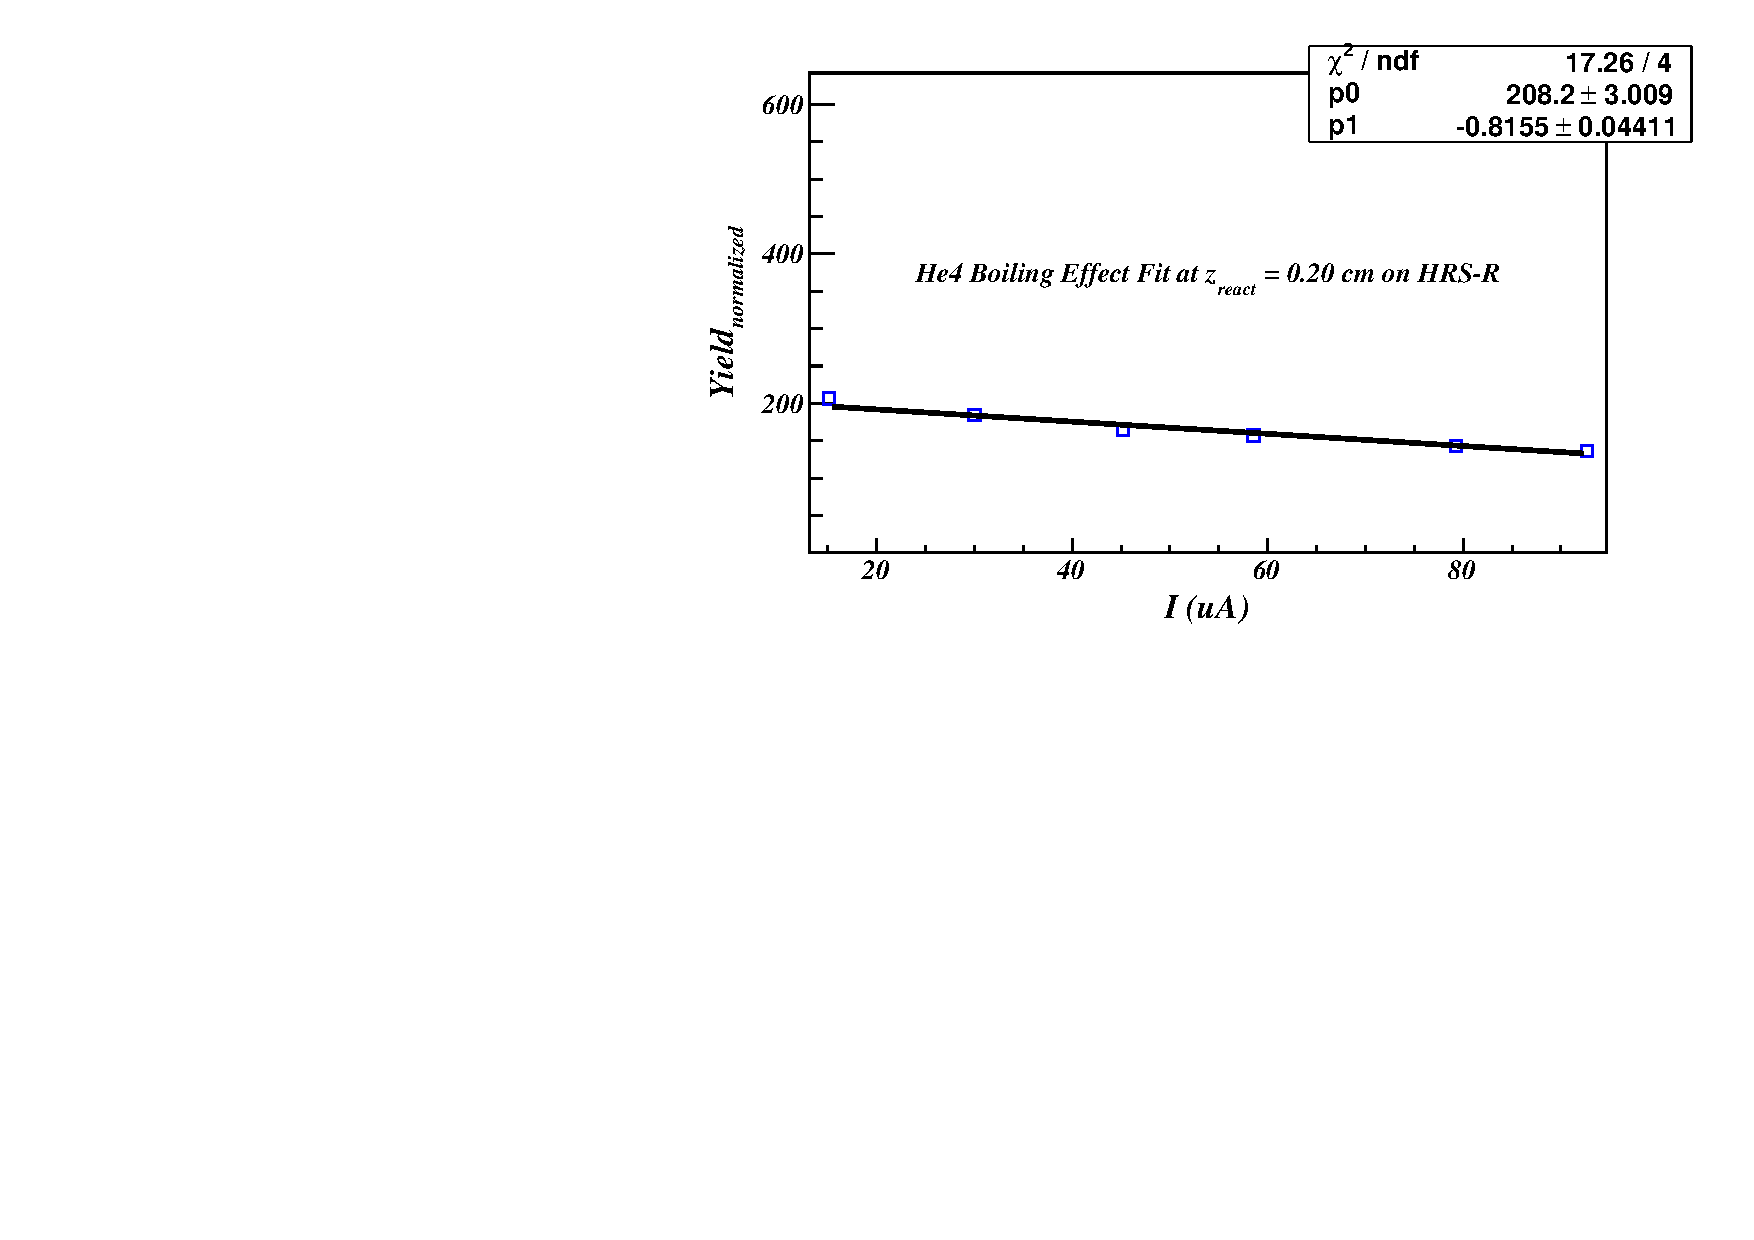
\includegraphics[type=pdf,ext=.pdf,read=.pdf,width=0.45\textwidth]{./figures/cryo/He4_Yield_R_All_0} 
    }
    \caption[Cryo-targets boiling effect fitting]{\footnotesize{Cryo-targets boiling effect fitting. They are examples near the center of the targets. Each target was divided into 60 bins along the target cell, where the boiling factor was individually fitted. The yield values have been normalized by a common factor.}}
    \label{cryo_boil_fit}
  \end{center}
\end{figure}
\begin{figure}[!h]
  \begin{center}
    \subfloat[$\mathrm{^{2}H2}$]{
      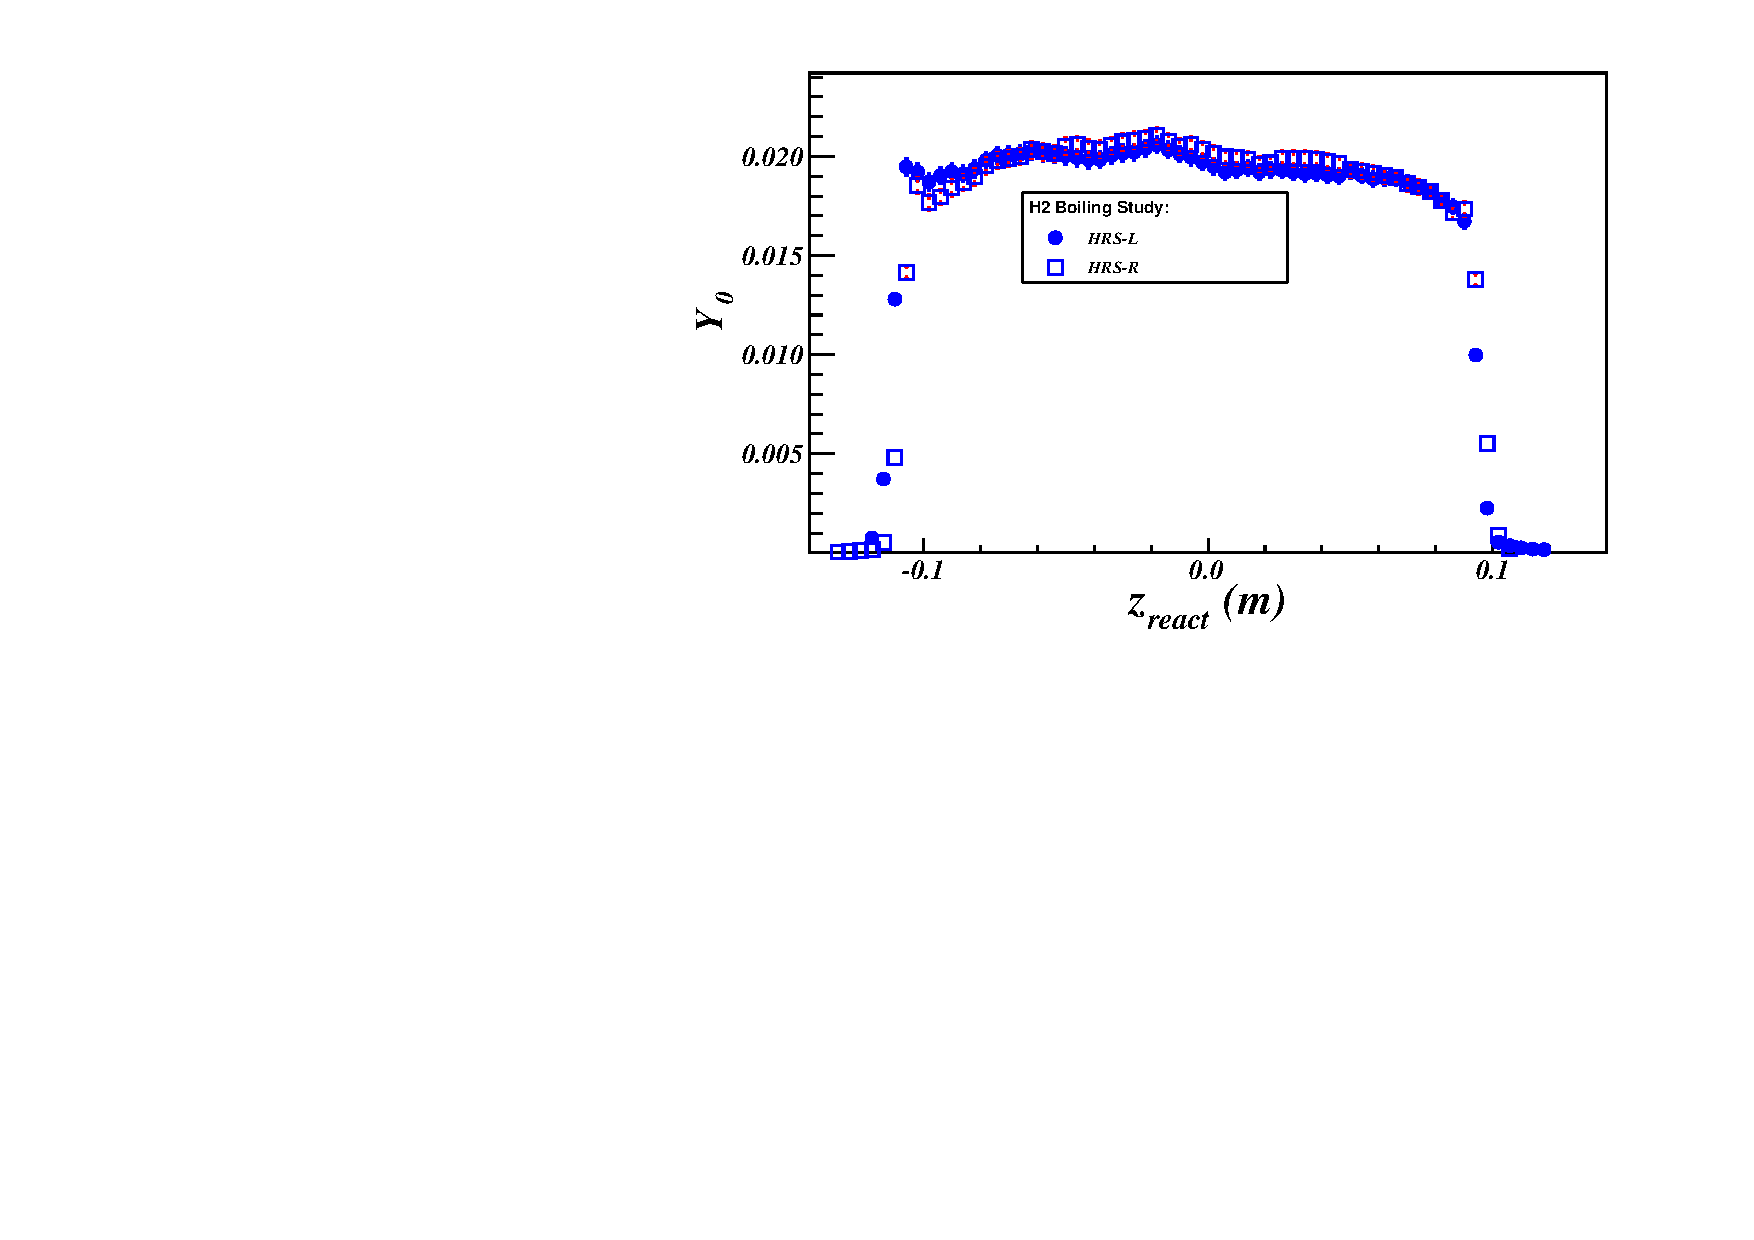
\includegraphics[type=pdf,ext=.pdf,read=.pdf,width=0.7\textwidth]{./figures/cryo/H2_Const} 
    }
    \hfill
    \subfloat[$\mathrm{^{3}He}$]{
      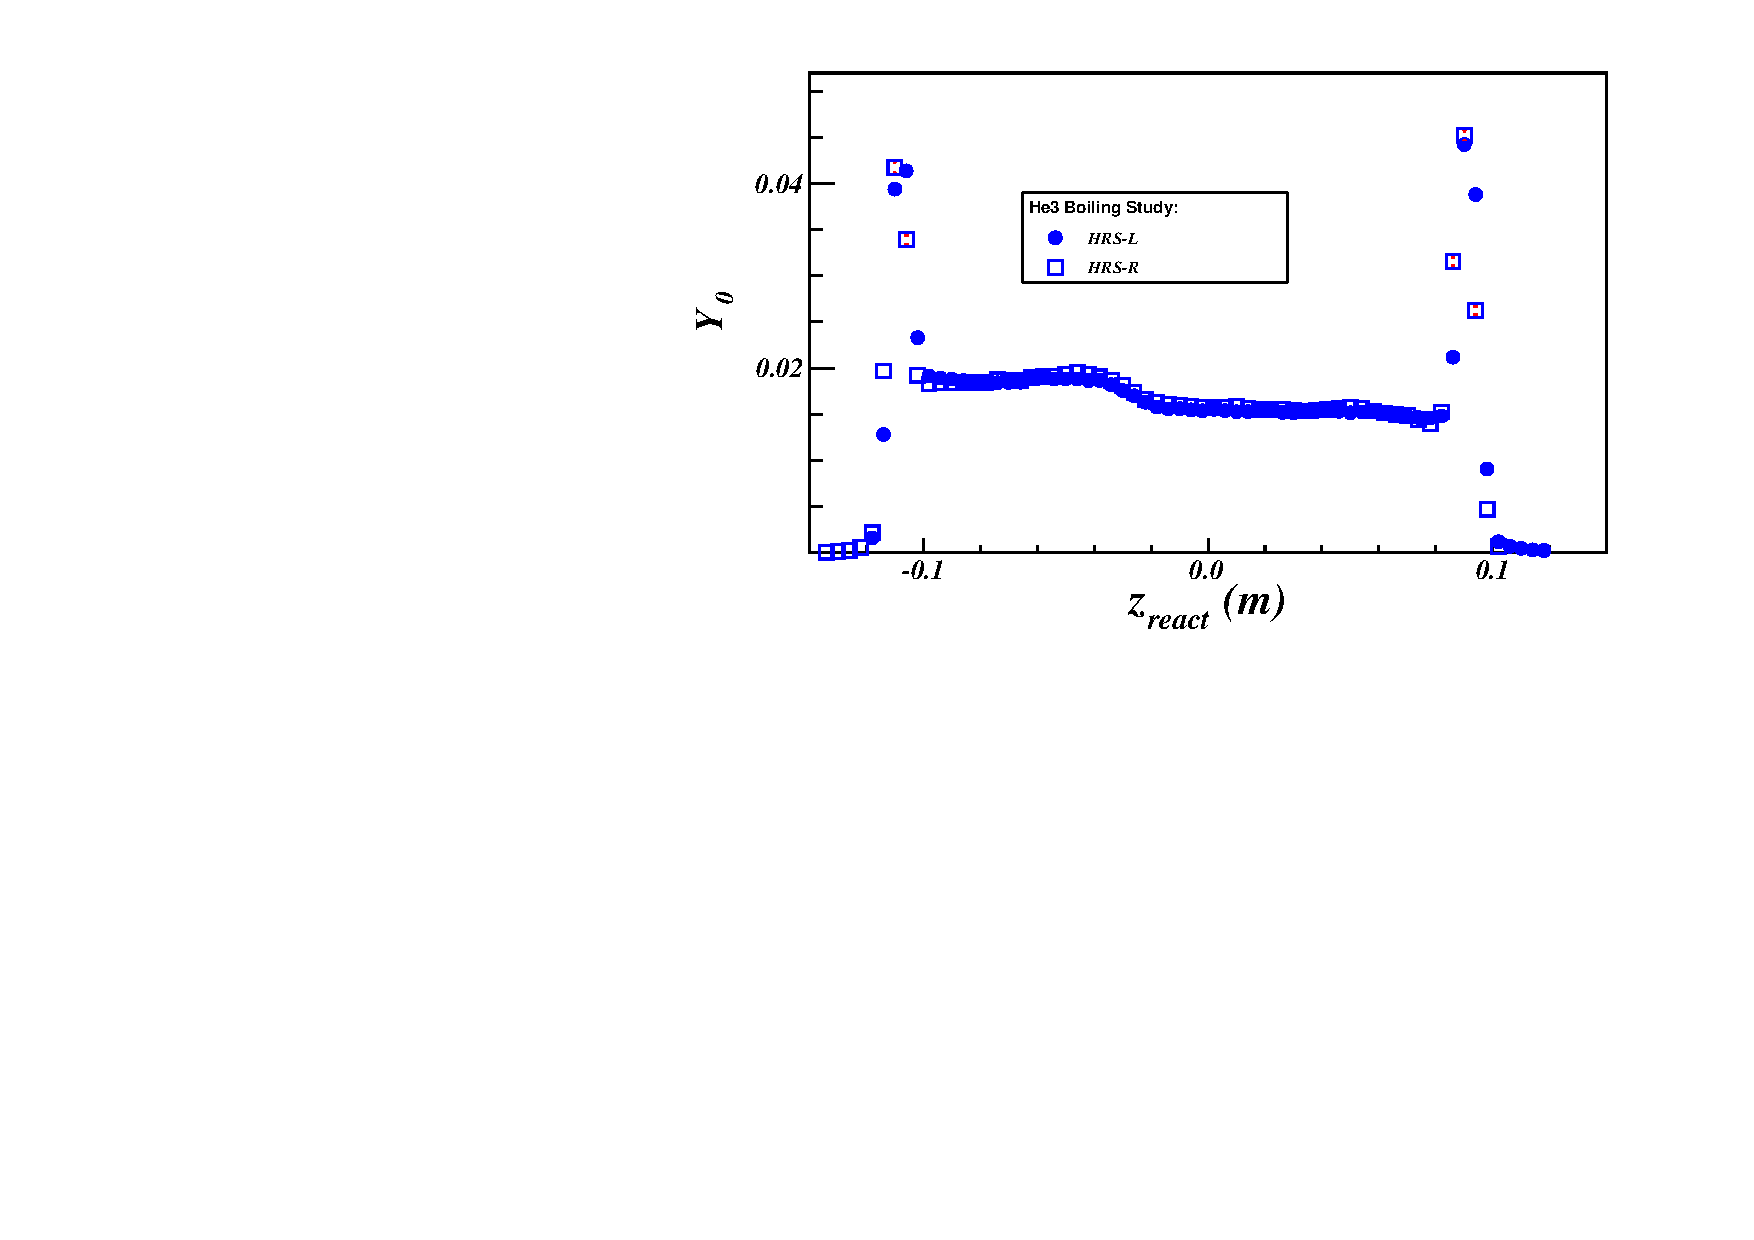
\includegraphics[type=pdf,ext=.pdf,read=.pdf,width=0.7\textwidth]{./figures/cryo/He3_Const} 
    }
     \hfill
    \subfloat[$\mathrm{^{4}He}$]{
      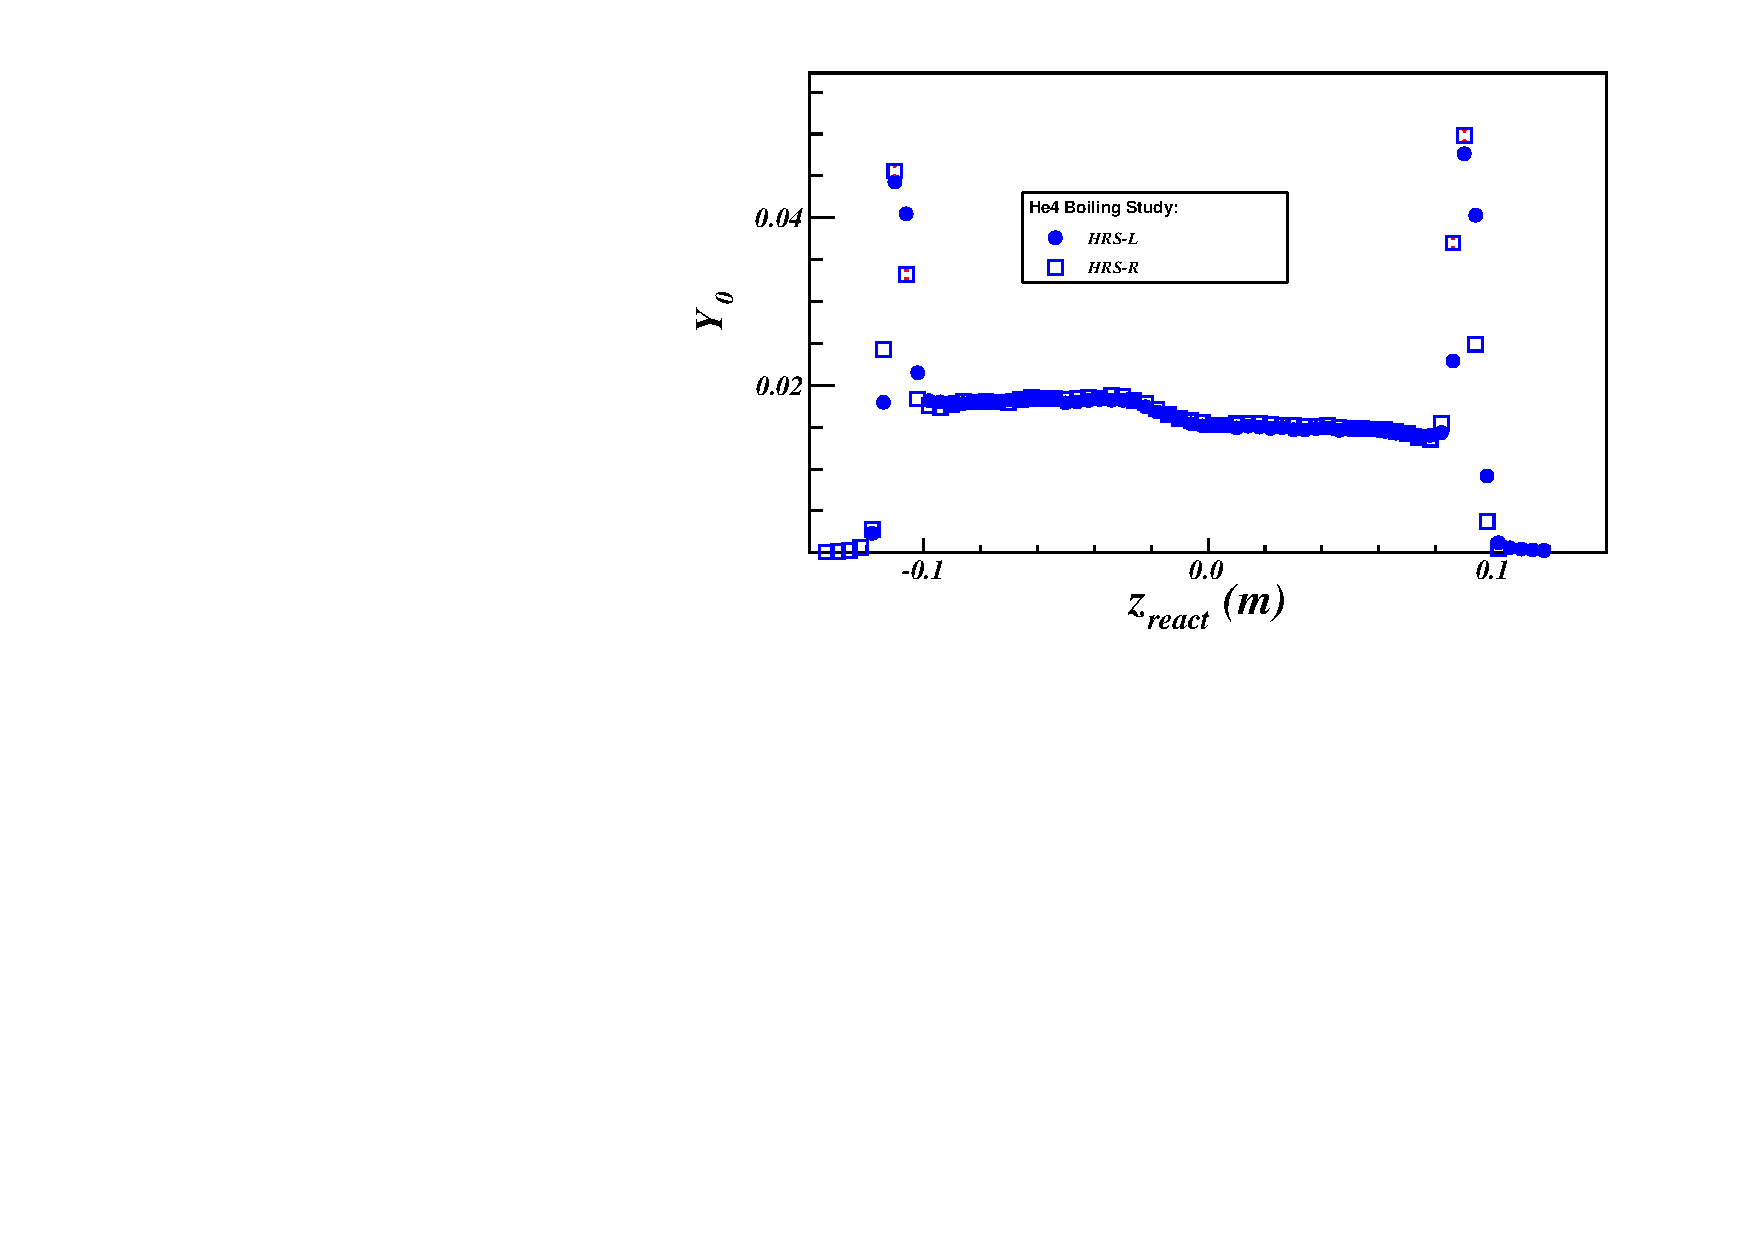
\includegraphics[type=pdf,ext=.pdf,read=.pdf,width=0.7\textwidth]{./figures/cryo/He4_Const} 
    }
    \caption[Cryo-target density profiles from the boiling study]{\footnotesize{Cryo-target density profiles from the boiling study. The results from both HRSs agree with each other for each target, and the peaks denote the contributions from the endcaps of the target cell.}}
    \label{cryo_boil_y0}
  \end{center}
\end{figure}

 Shown in Fig.~\ref{c12_boil_fit}, the fitting result of $\mathrm{^{12}C}$ indicates that for a fixed target density, the yield does not change at different current. For cryo-target, the data was binned in $z_{react}$ which was divided into 60 bins. In each bin, the yield was calculated and one can fit the boiling factor by the formula:
 \begin{equation}
  Y(I, z_{react}^{i}) = Y(0, z_{react}^{i}) + m(z_{react}^{i})\cdot I,,\quad where~i=1,\cdots,60,
  \label{eq_yield_rho_zbin}
\end{equation}
which gives the variation of the density in each bin:
 \begin{equation}
  \rho(I, z_{react}^{i}) = \rho(0, z_{react}^{i}) \cdot (1.0 + BF(z_{react}^{i}) \cdot I /100),
  \label{eq_rho_zbin}
 \end{equation}
where,
 \begin{equation}
   BF(z_{react}^{i})=\frac{Y(0, z_{react}^{i})}{m(z_{react}^{i})}. \\
     \label{eq_bf_zbin}
 \end{equation}

As examples, Fig.~\ref{cryo_boil_fit} shows the fitting results of boiling factors at the center of $z_{react}$ for three cryo-targets, where the curves are well fitted by linear functions. The curve of normalized $Y(0, z_{react}^{i})$ denotes the target density profile along the cell, as shown in Fig.~\ref{cryo_boil_y0}, where the peaks of endcaps can be clearly seen. The distribution of $BF(z_{react}^{i})$ for each target, given in Fig.~\ref{cryo_boil_fact}, shows the boiling effects at different $z_{react}$, and demonstrates that the non-uniform cryo-target densities were mainly caused by the highly localized boiling effects. In the plot, the values of $z_{react}$ at the positions of endcaps are close to zero which agree with the fact that the density of aluminium walls shouldn't change with beam current. Results from both HRSs were compared and found out to agree nicely with each other. 
 \begin{figure}[]
  \begin{center}
    \subfloat[$\mathrm{^{2}H}$]{
      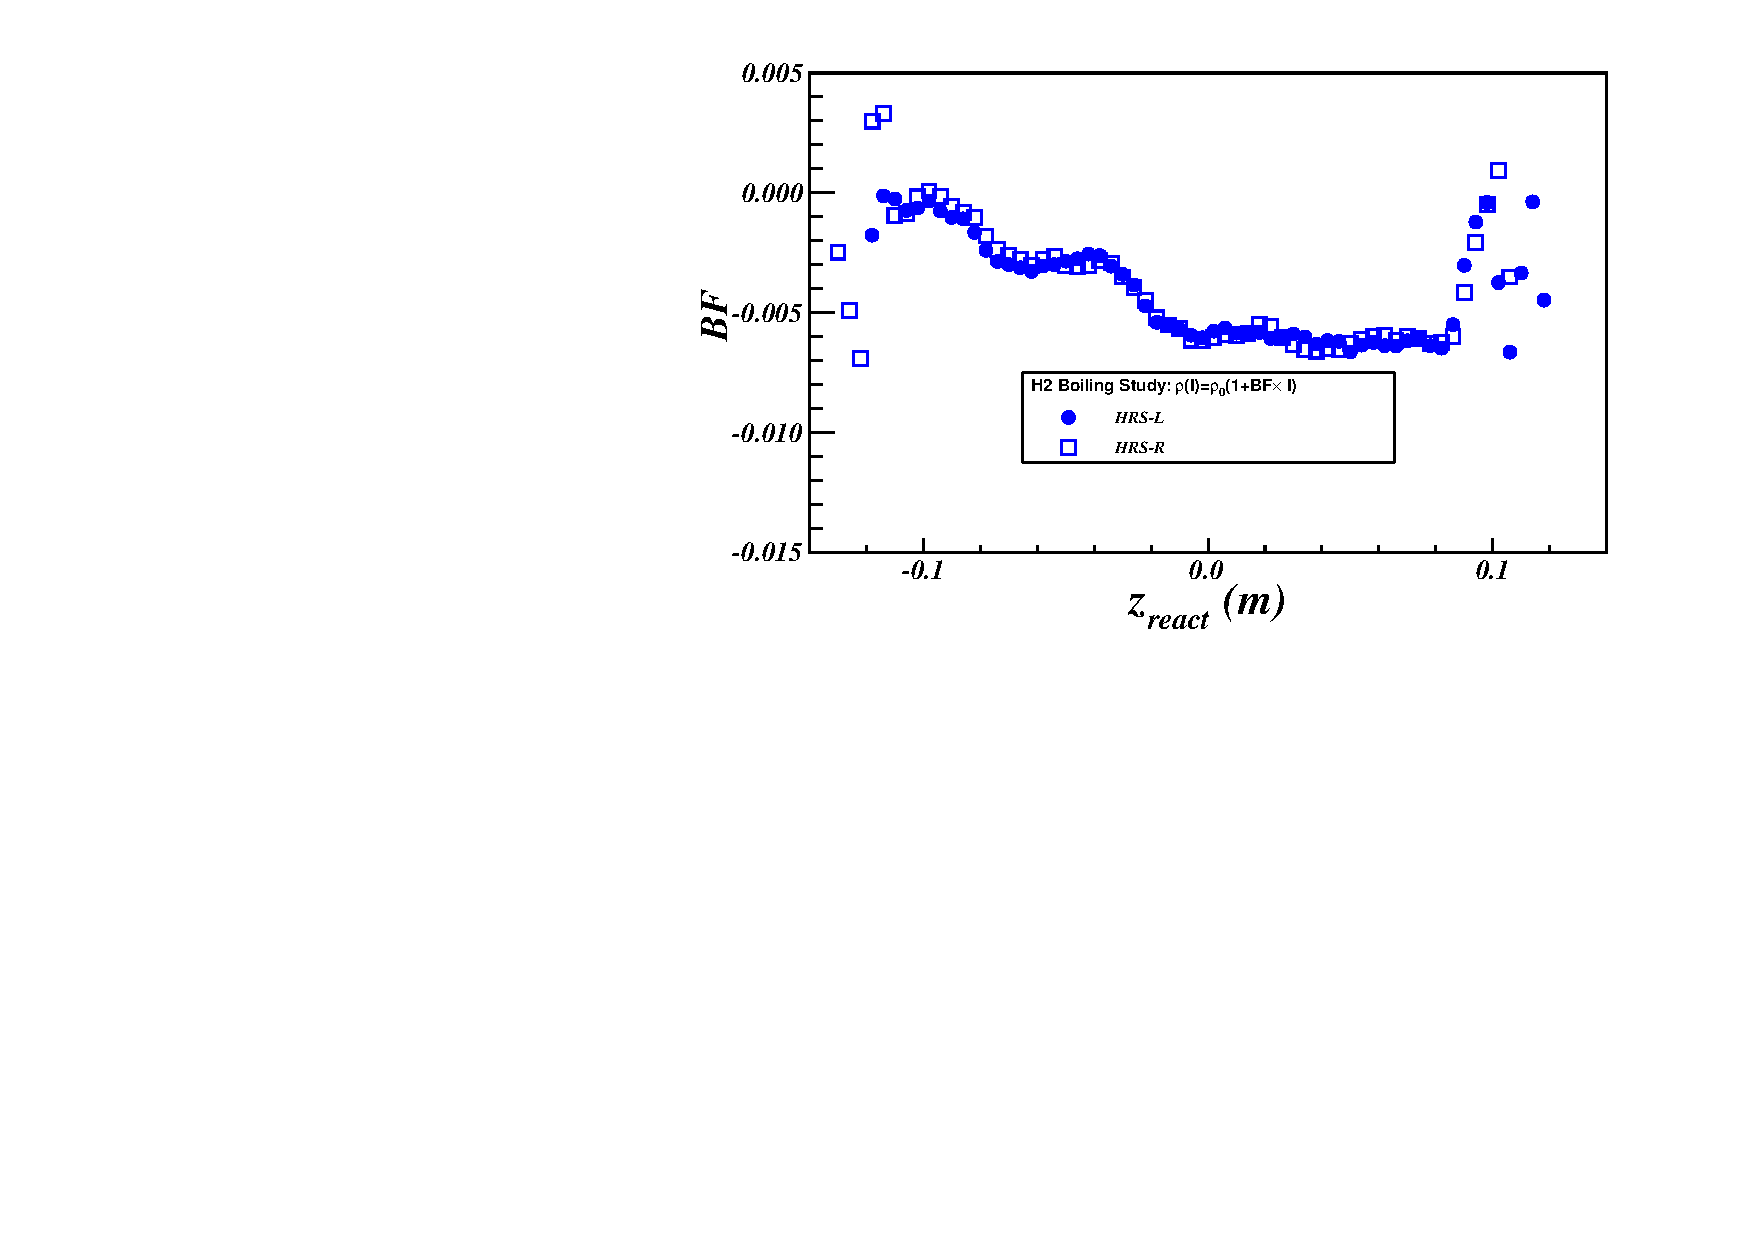
\includegraphics[type=pdf,ext=.pdf,read=.pdf,width=0.7\textwidth]{./figures/cryo/H2_BF} 
    }
    \hfill
    \subfloat[$\mathrm{^{3}He}$]{
      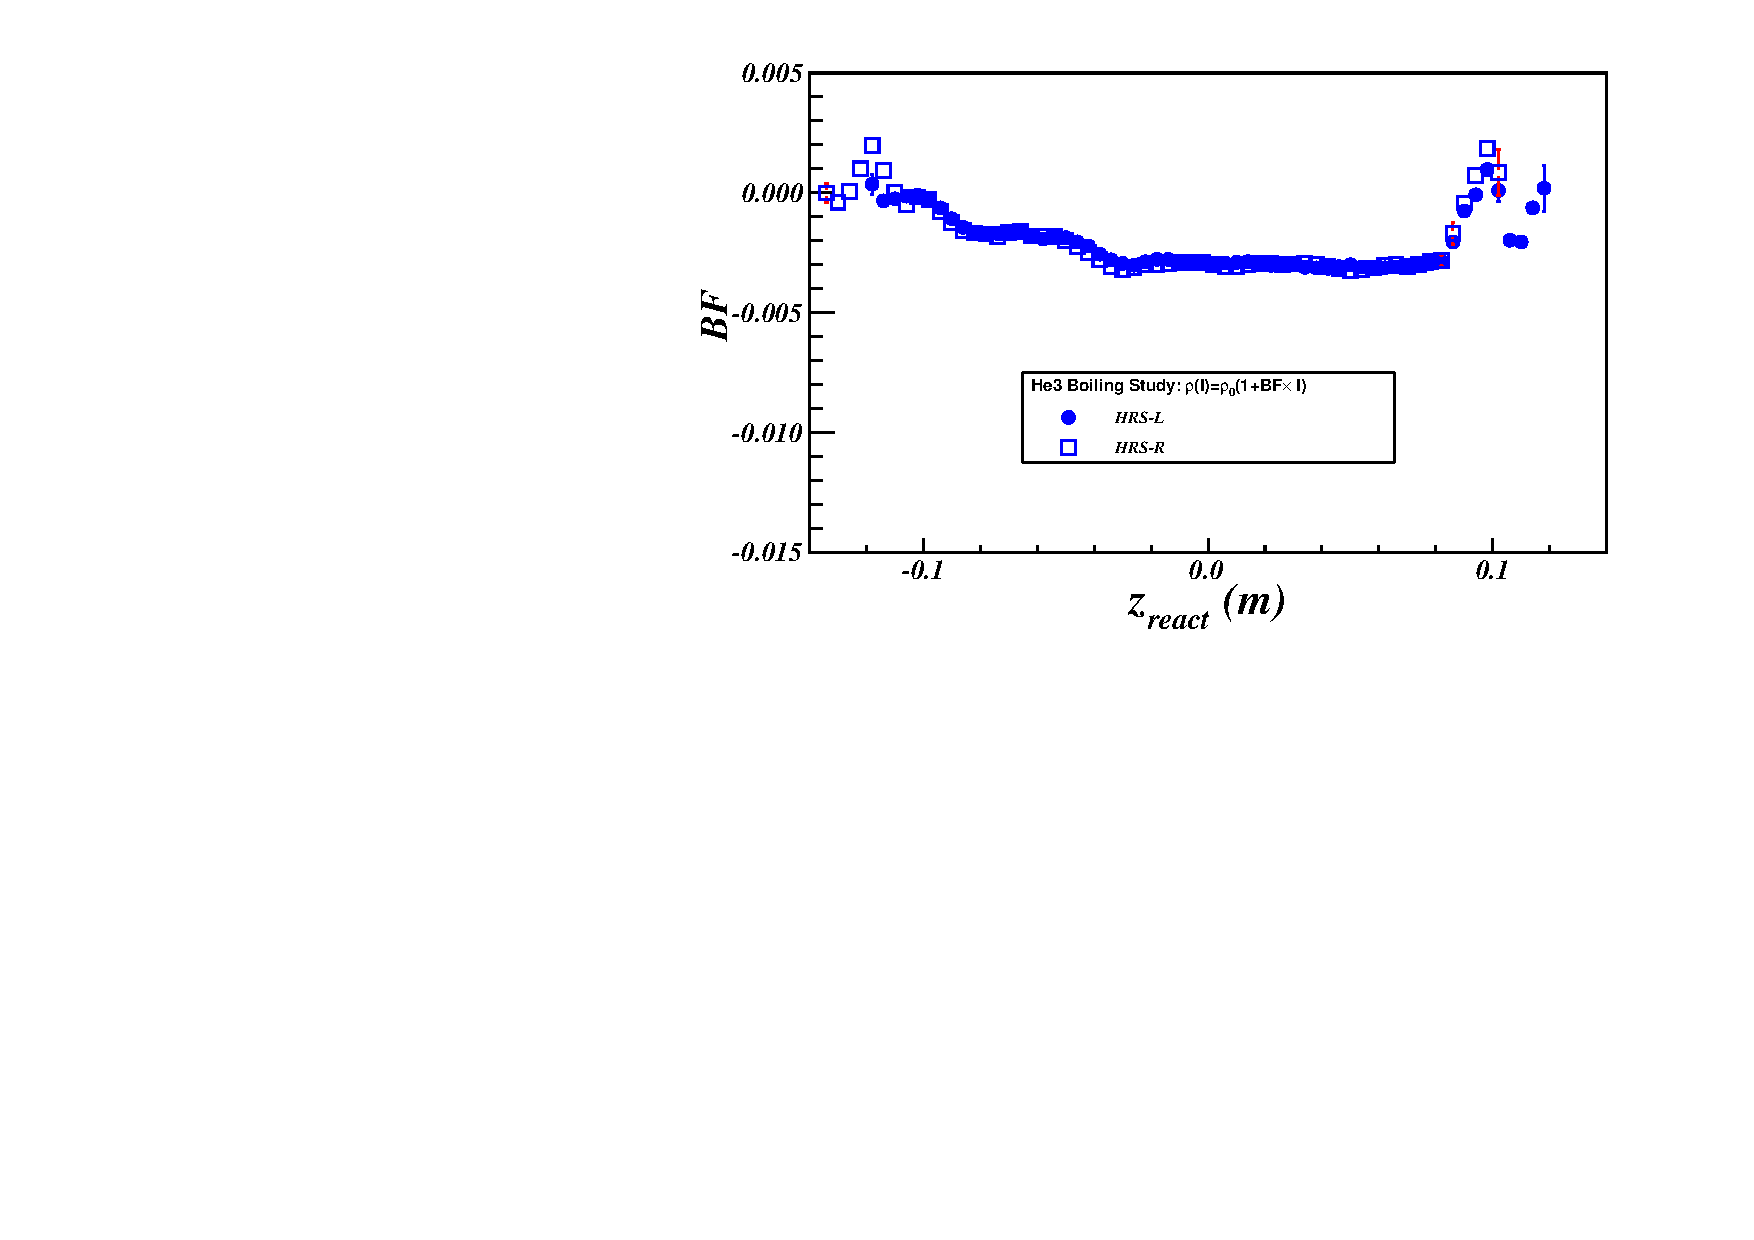
\includegraphics[type=pdf,ext=.pdf,read=.pdf,width=0.7\textwidth]{./figures/cryo/He3_BF} 
    }
     \hfill
    \subfloat[$\mathrm{^{4}He}$]{
      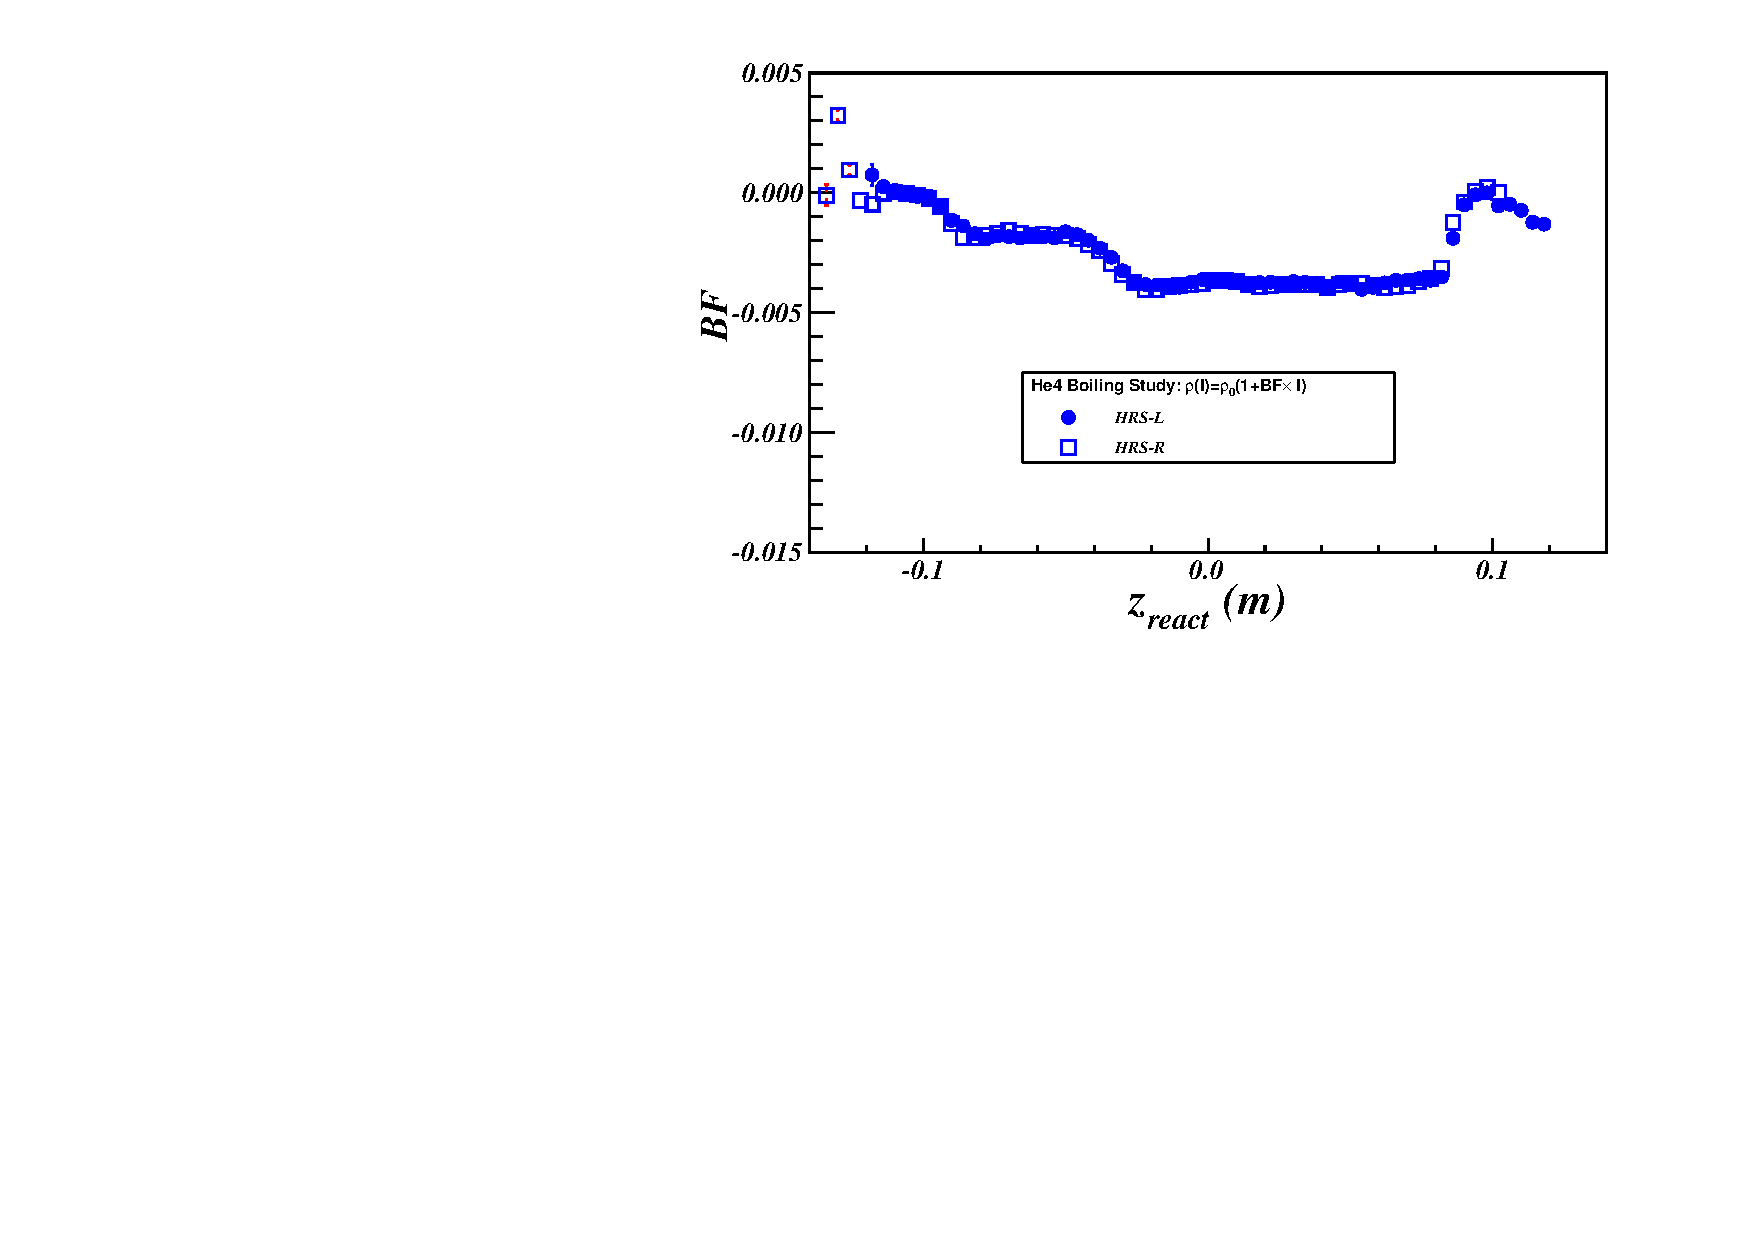
\includegraphics[type=pdf,ext=.pdf,read=.pdf,width=0.7\textwidth]{./figures/cryo/He4_BF} 
    }
    \caption[Cryo-target boiling factor distribution]{\footnotesize{Cryo-target boiling factor distribution. Each plot clearly shows that the boiling effect varies along the target cells. The boiling factors at the endcaps are reasonably close to zero. The studies from both HRSs give consistent results. The yield values had been normalized by a common factor.}}
    \label{cryo_boil_fact}
  \end{center}
\end{figure}

\section{Extracting Density Distributions}
  From Eq.~\eqref{eq_yield_rho_zbin}, the target density profile can be obtained by extracting the distribution of $Y(0)$ during the boiling study. In this section, a different method is applied to extract the density distribution by with the experimental data and simulation data. 
  
  Since $z_{react}$ is along the incoming beam direction so as the orientation of the target cell, the $z_{react}$ distribution in the experimental data, $z_{react}^{EX}$, gives the distribution of yields in one current setting. Meanwhile, the yield for one $z_{react}^{EX}$ value is proportional to the density of the target in this location, so one expects to study the density distribution of the target with the $z_{react}^{EX}$ distribution. However, $z_{react}^{EX}$ should also contain the acceptance effect of the HRS and the cross section weighting effect. One can use the simulation data generated by SAMC which simulates the acceptance effect of HRSs, and plot the simulated $z_{react}$ distribution, $z_{react}^{MC}$. One can further weight $z_{react}^{MC}$ by the cross section values calculated from XEMC. When the target density distribution in the simulation data is uniform, $z_{react}^{MC}$ only carries the acceptance effect and the cross section effect. By plotting the histograms of $z_{react}^{EX}$ and $z_{react}^{MC}$ with the same range and bin-size, one takes to ratio of two histogram, which leads to a clean relative density distribution of the target at the current setting.
  
   The plots on the left hand side of Fig.~\ref{cryo_den_fit} show the distribution of $z_{react}^{EX}$ and $z_{react}^{MC}$ at three different current settings for each target, while the plots on the right hand side give the fitting results of the relative density distributions. A polynomial function is used for each fitting process. 
 \begin{figure}[!ht]
  \begin{center}
    \subfloat[$\mathrm{^{2}H}$]{
      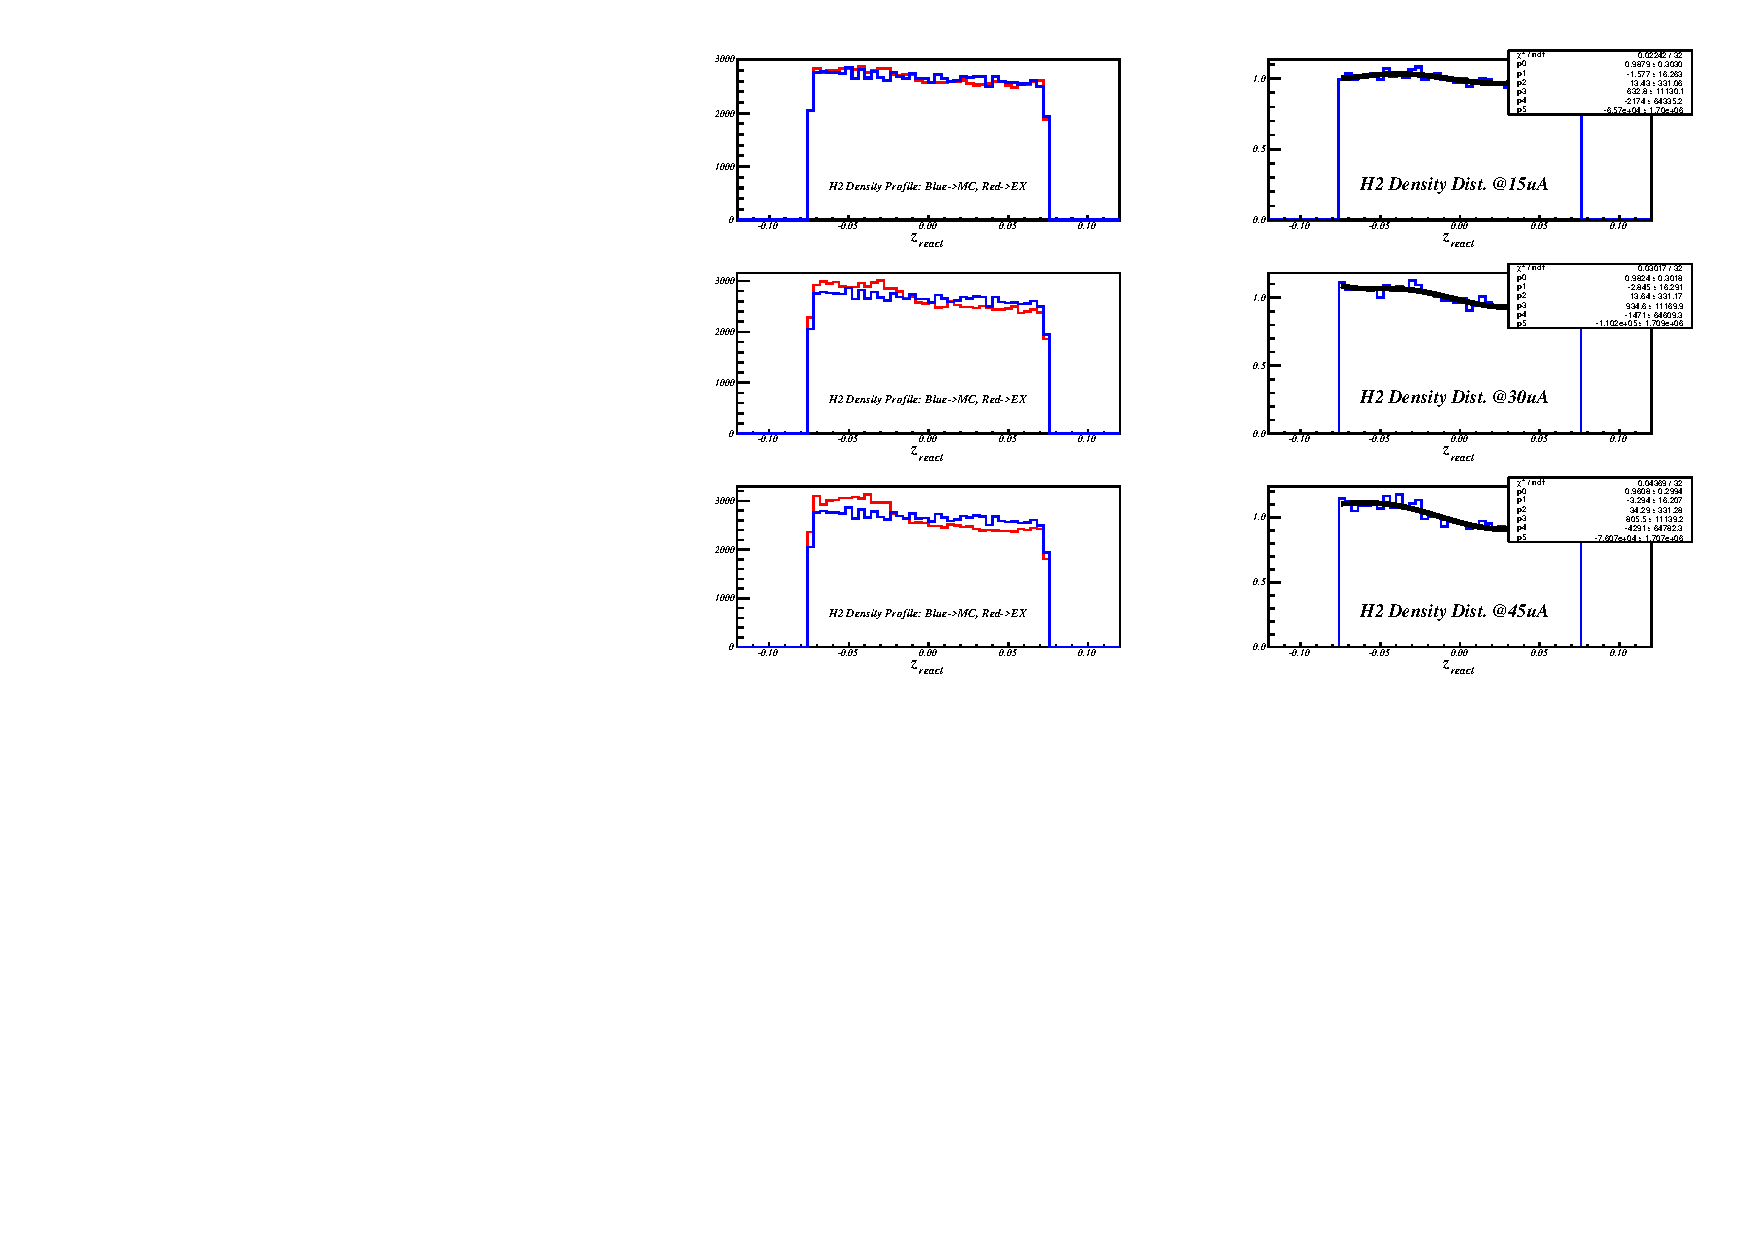
\includegraphics[type=pdf,ext=.pdf,read=.pdf,width=0.7\textwidth]{./figures/cryo/H2_Boiling_Density} 
    }
    \hfill
    \subfloat[$\mathrm{^{3}He}$]{
      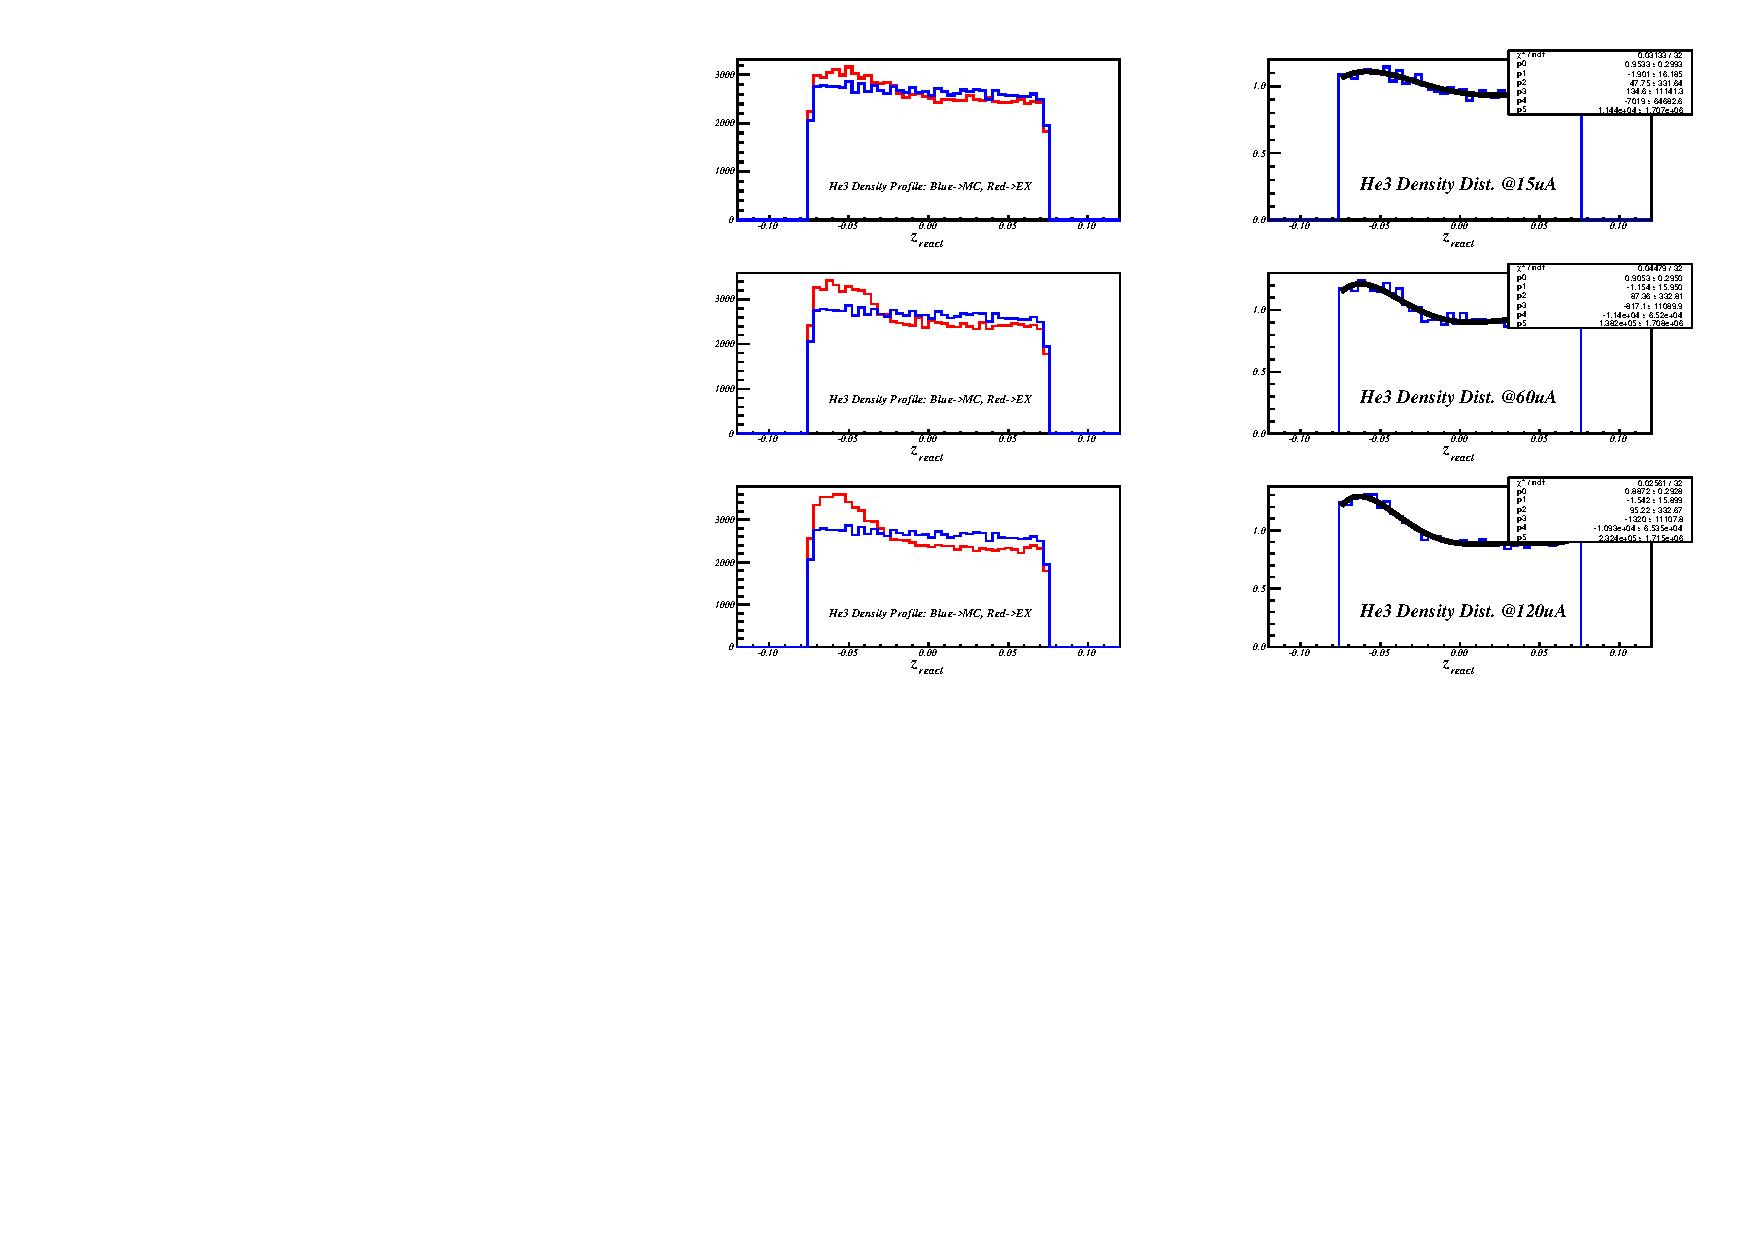
\includegraphics[type=pdf,ext=.pdf,read=.pdf,width=0.7\textwidth]{./figures/cryo/He3_Boiling_Density} 
    }
     \hfill
    \subfloat[$\mathrm{^{4}He}$]{
      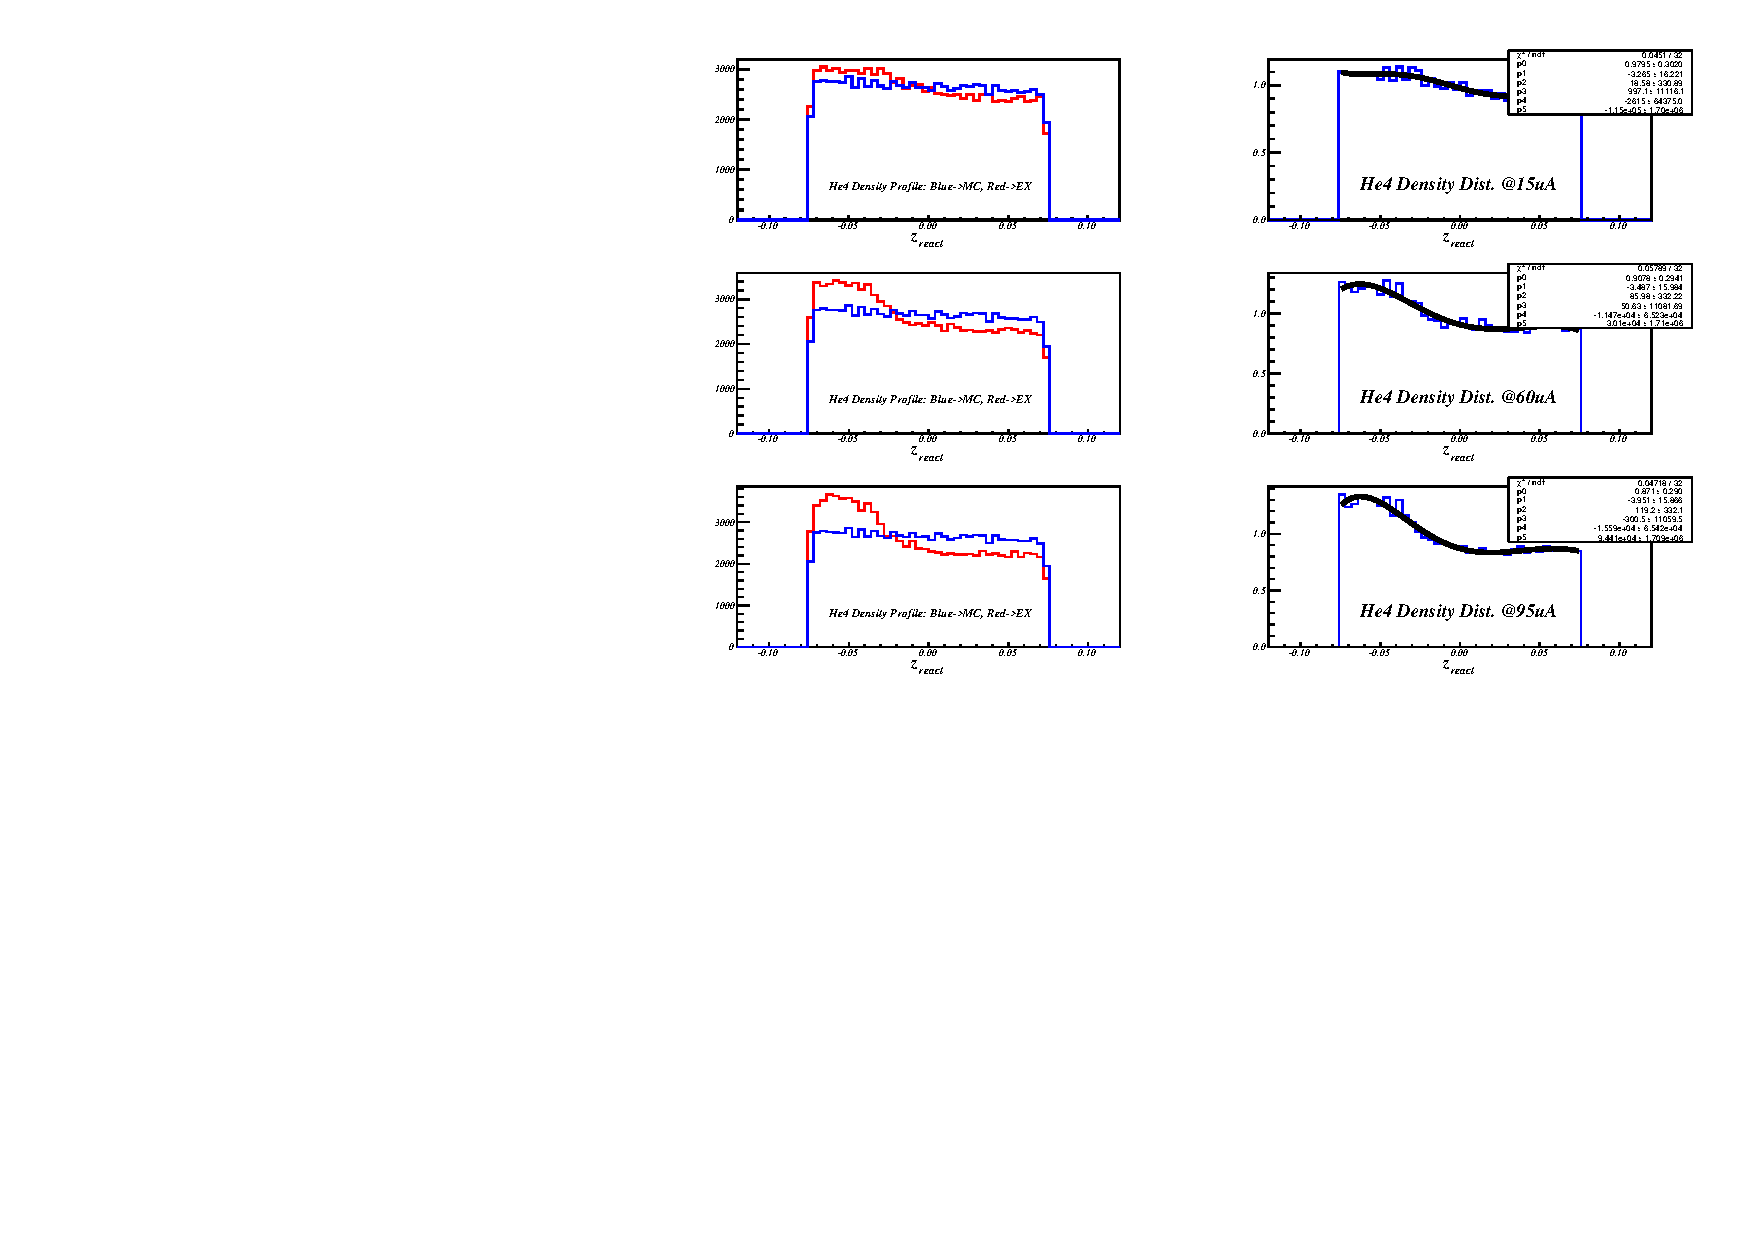
\includegraphics[type=pdf,ext=.pdf,read=.pdf,width=0.7\textwidth]{./figures/cryo/He4_Boiling_Density} 
    }
    \caption[Cryo-target density distributions extracted from data]{\footnotesize{Cryo-target density distributions extracted from data. The density distribution was extracted by taking the histogram ratio of $z_{react}$ from experimental data (red lines in plots on the left panel) and from simulation data with flat density distribution (blue lines in plots on the left panel). For each target, the density distributions at the minimum, middle and maximum currents were individually extracted (on right panel). The current settings are given in the plots.}}
    \label{cryo_den_fit}
  \end{center}
\end{figure}

 One can use the density distributions at the minimum current (15 uA, 20 uA and 15 uA for $\mathrm{^{2}H}$, $\mathrm{^{3}He}$ and $\mathrm{^{4}He}$, respectively), and apply the boiling factors to calculate the density distribution at beam current equal to zero, $\rho(0)$. Then the density distribution at any current settings, $\rho_{Calc}(I)$ can be calculated with Eq.~\eqref{eq_rho_zbin}. To verify the boiling study results and the density distributions at different current settings, the distributions of $\rho_{Calc}(I)$ and $\rho(I)$ extracted in Fig.~\ref{cryo_den_fit} were compared, as shown in Fig.~\ref{cryo_den_comp}. Note that the contributions from the two endcaps were removed by applying the cut, $|z_{react}|\leq 7.5~cm$. The plots reveal that the results of boiling study successfully characterize the change of target density with different beam currents.
  \begin{figure}[!ht]
  \begin{center}
    \subfloat[$\mathrm{^{2}H}$ at I=30 uA]{
      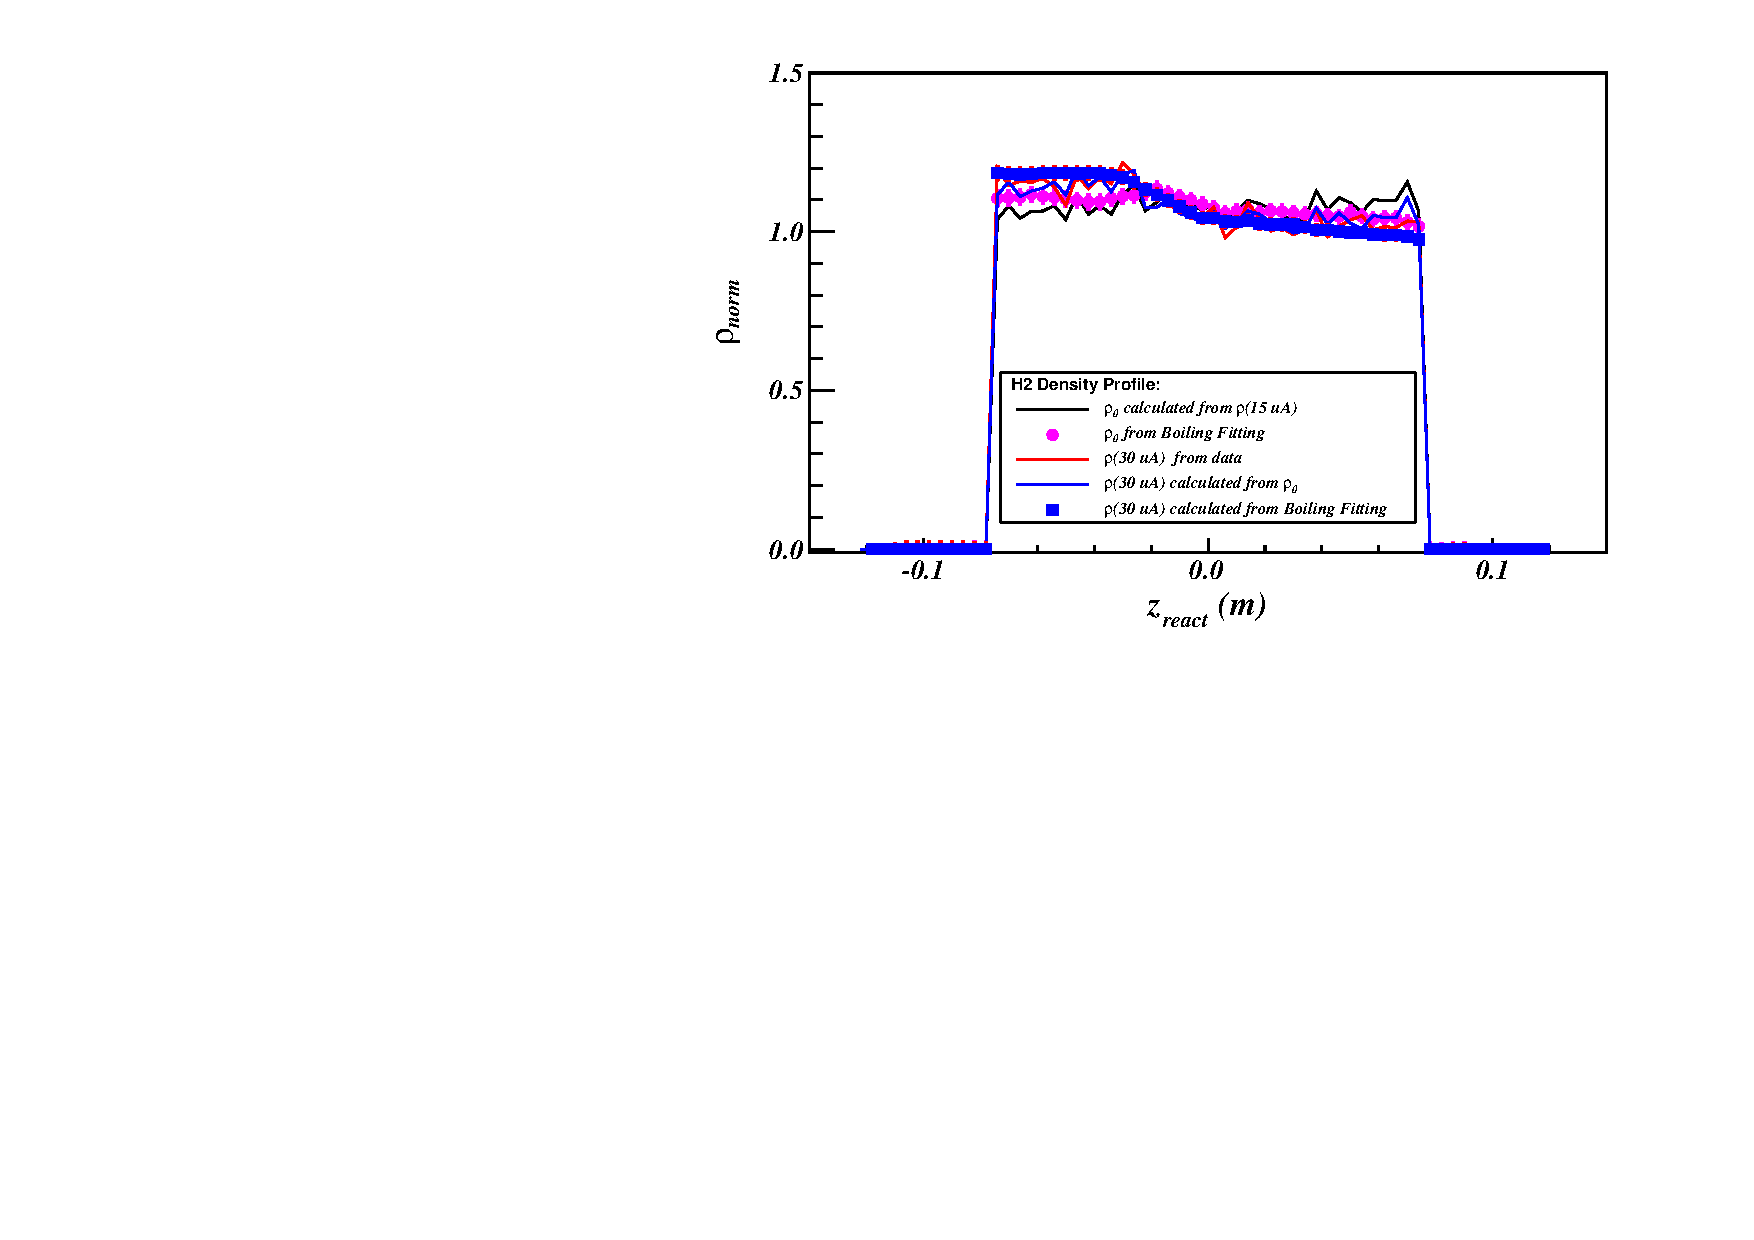
\includegraphics[type=pdf,ext=.pdf,read=.pdf,width=0.45\textwidth]{./figures/cryo/H2_Check_30} 
    }
    \hfill
    \subfloat[$\mathrm{^{2}H}$ at I=45 uA]{
      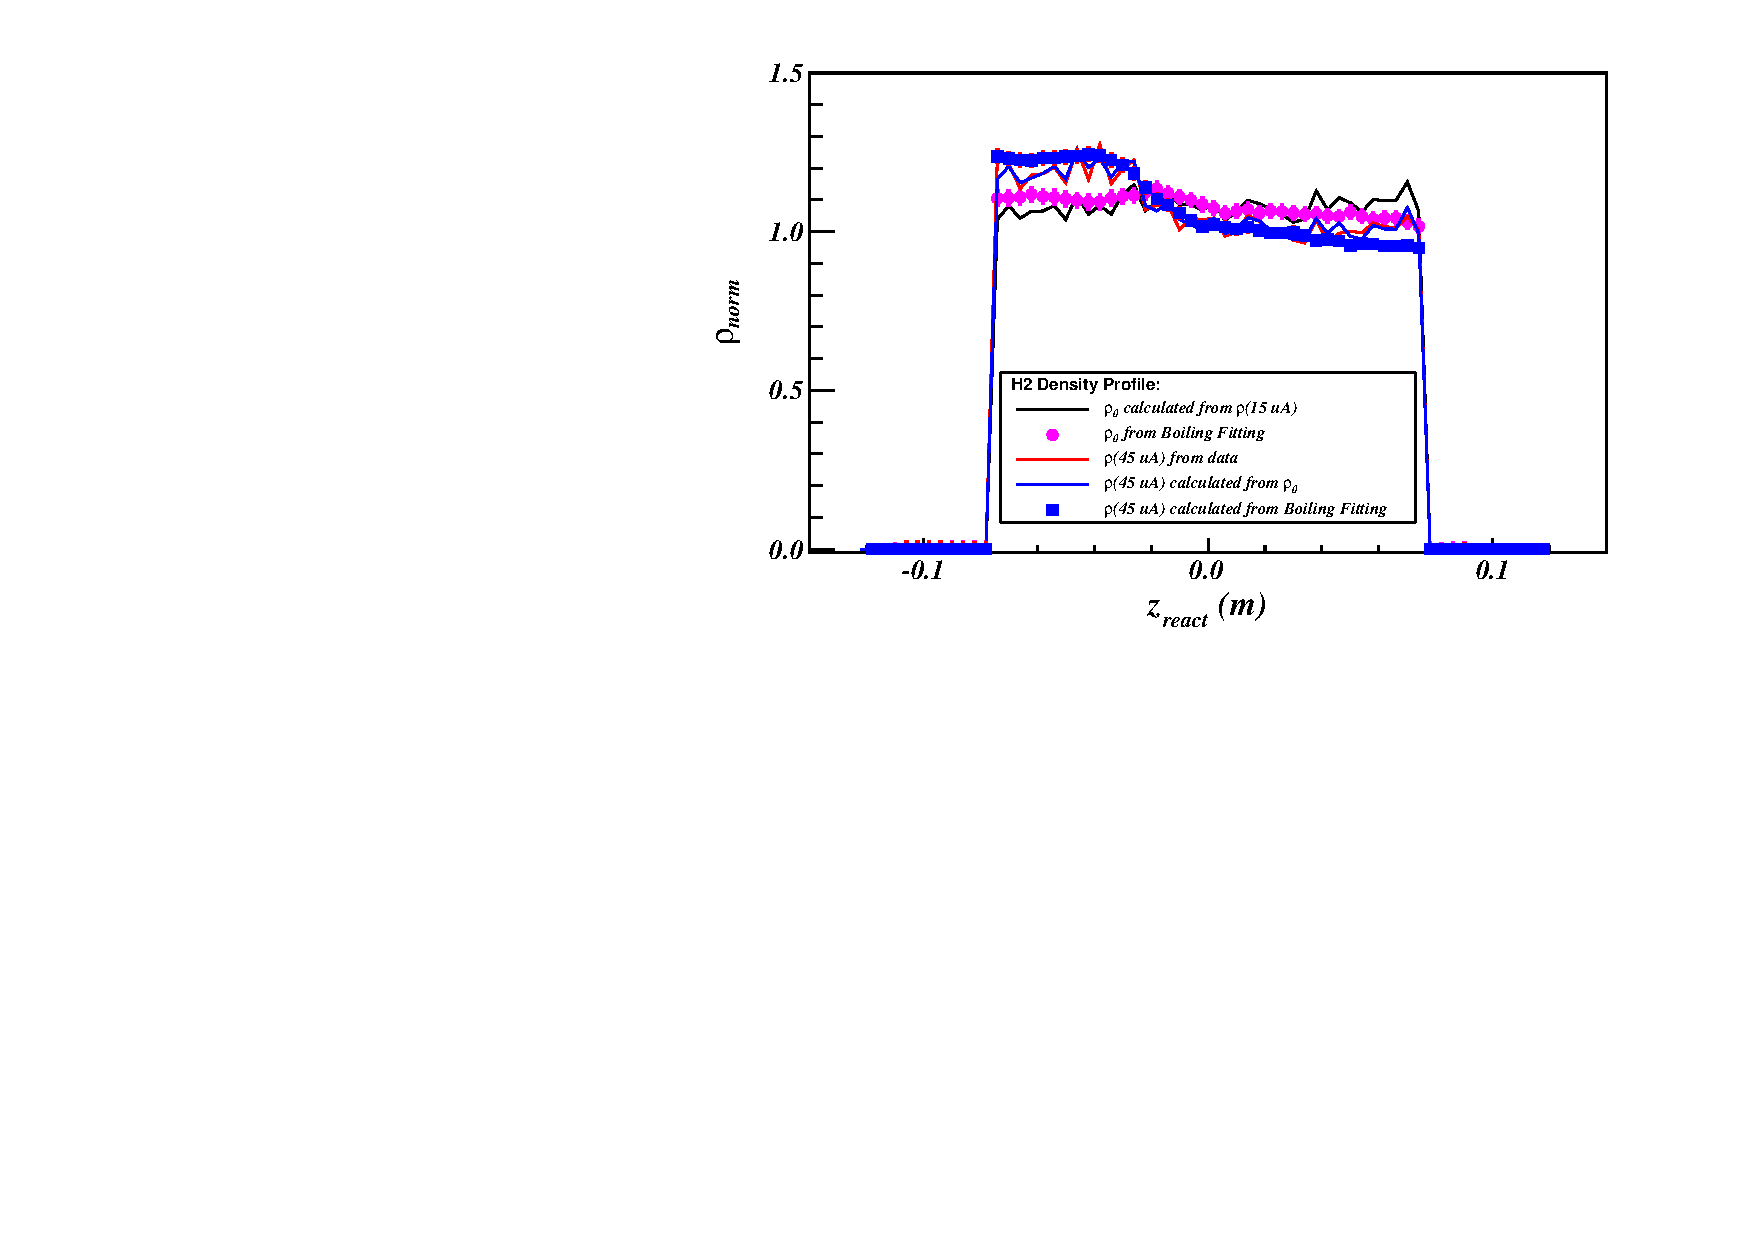
\includegraphics[type=pdf,ext=.pdf,read=.pdf,width=0.45\textwidth]{./figures/cryo/H2_Check_45} 
    }
\\
    \subfloat[$\mathrm{^{3}He}$ at I=60 uA]{
      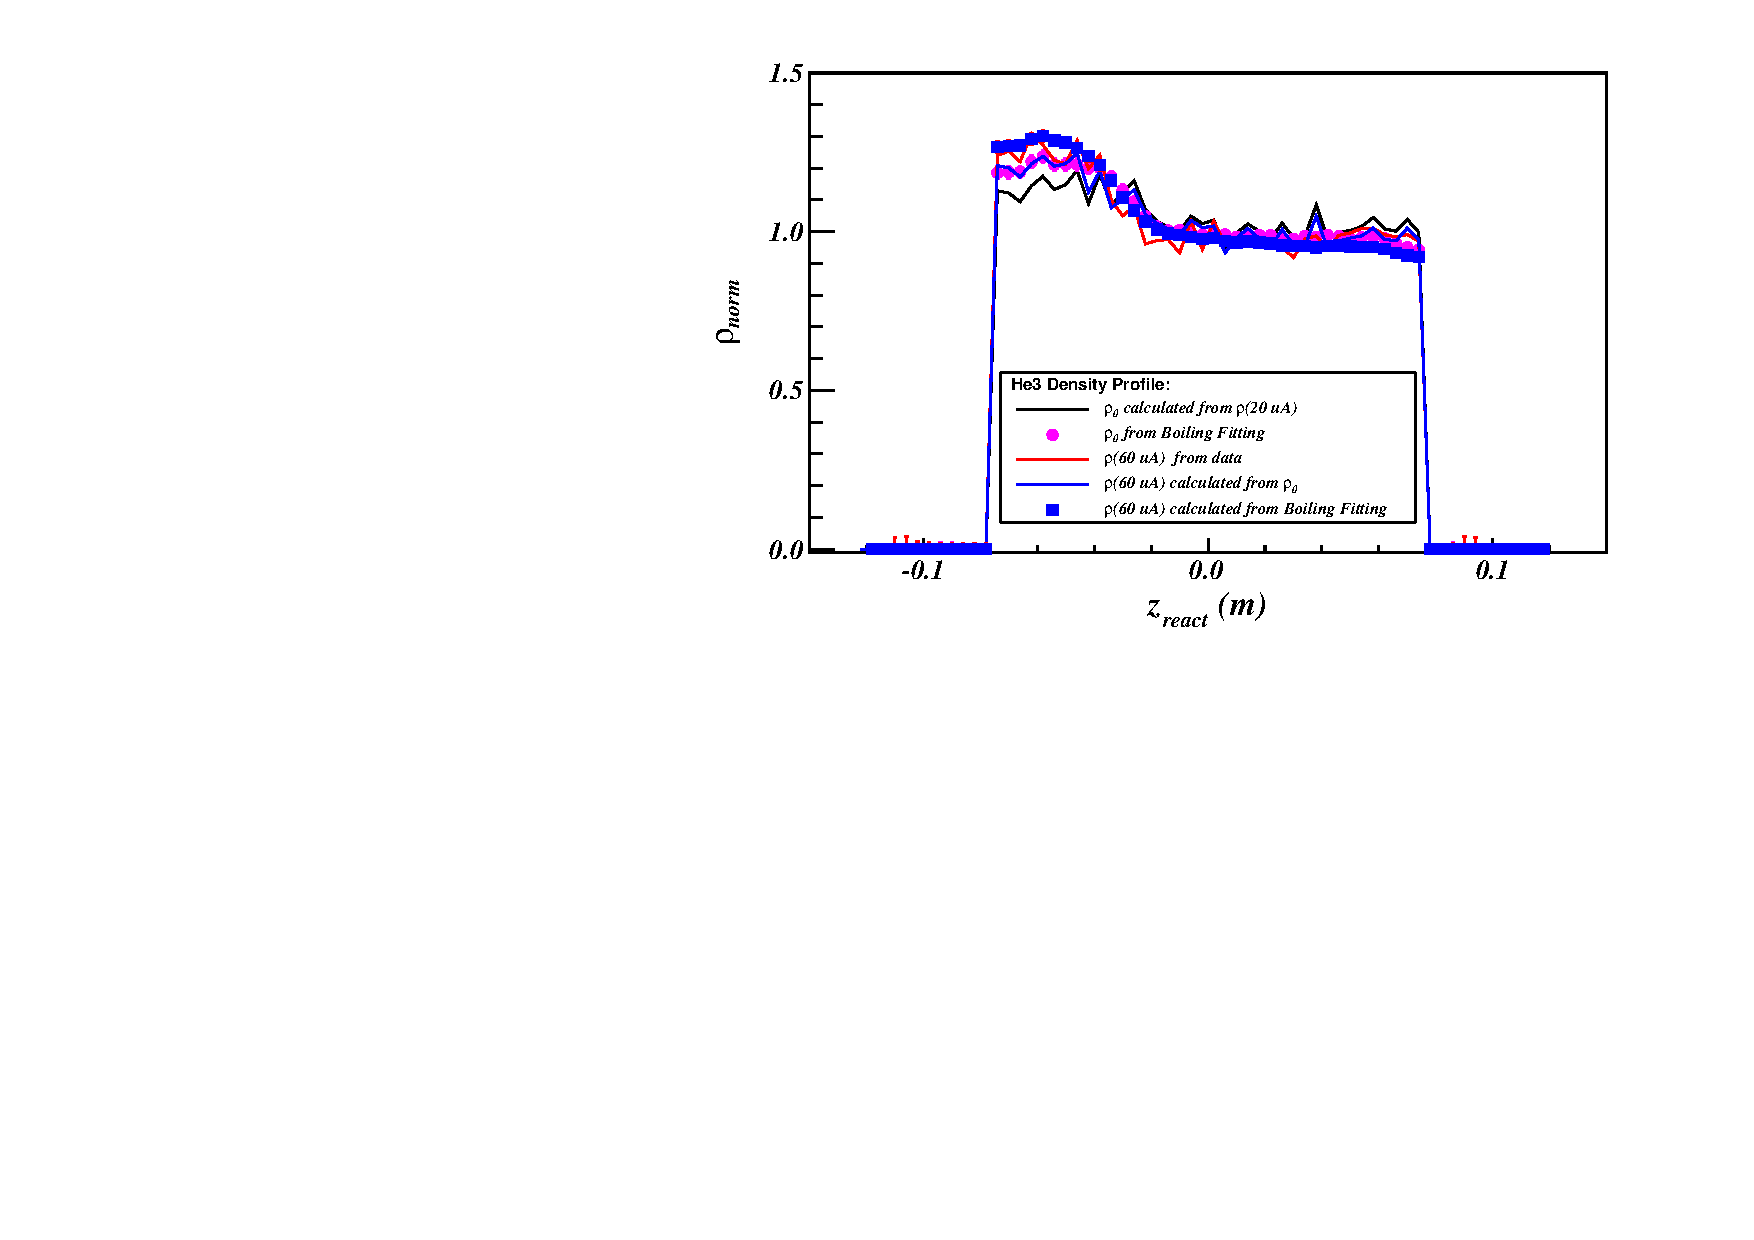
\includegraphics[type=pdf,ext=.pdf,read=.pdf,width=0.45\textwidth]{./figures/cryo/He3_Check_60} 
    }
    \hfill
    \subfloat[$\mathrm{^{3}He}$ at I=120 uA]{
      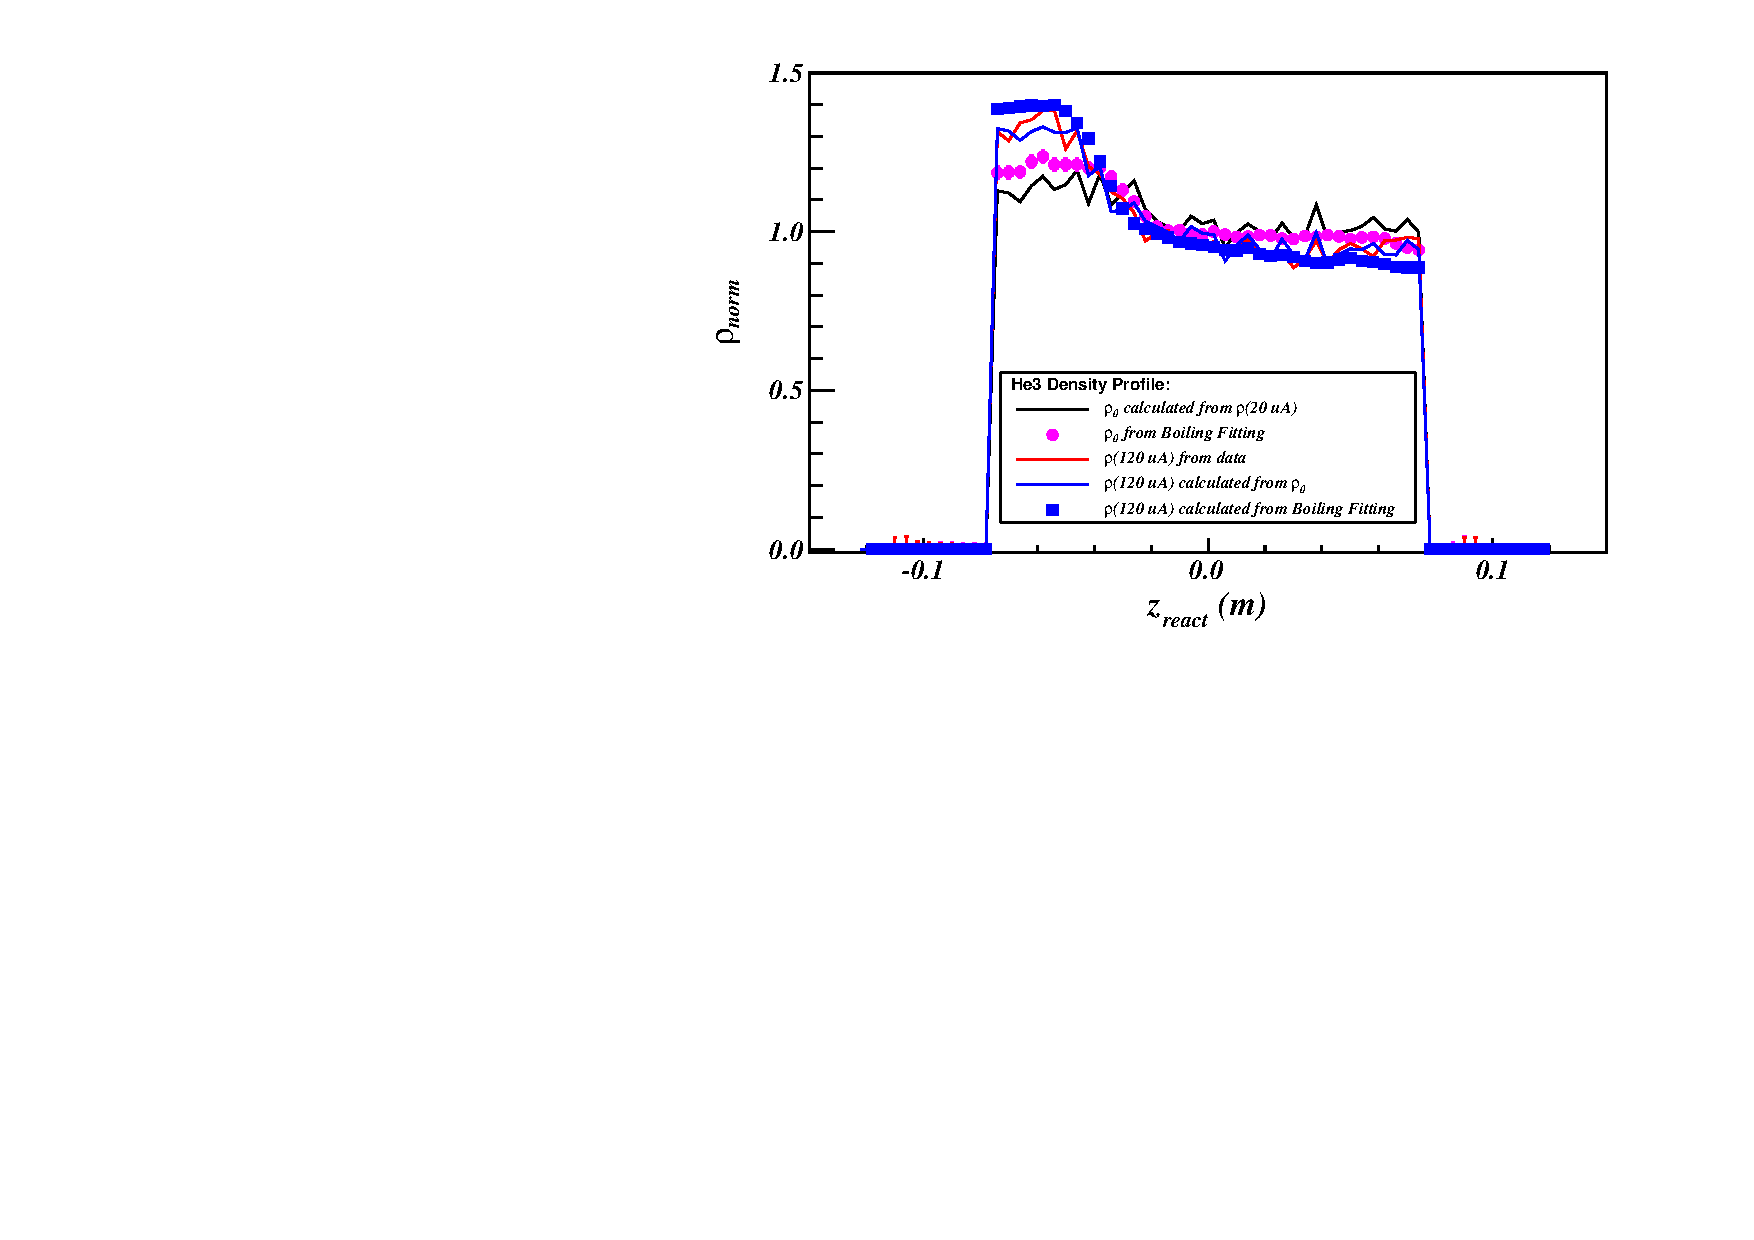
\includegraphics[type=pdf,ext=.pdf,read=.pdf,width=0.45\textwidth]{./figures/cryo/He3_Check_120} 
    }
\\
    \subfloat[$\mathrm{^{4}He}$ at I=60 uA]{
      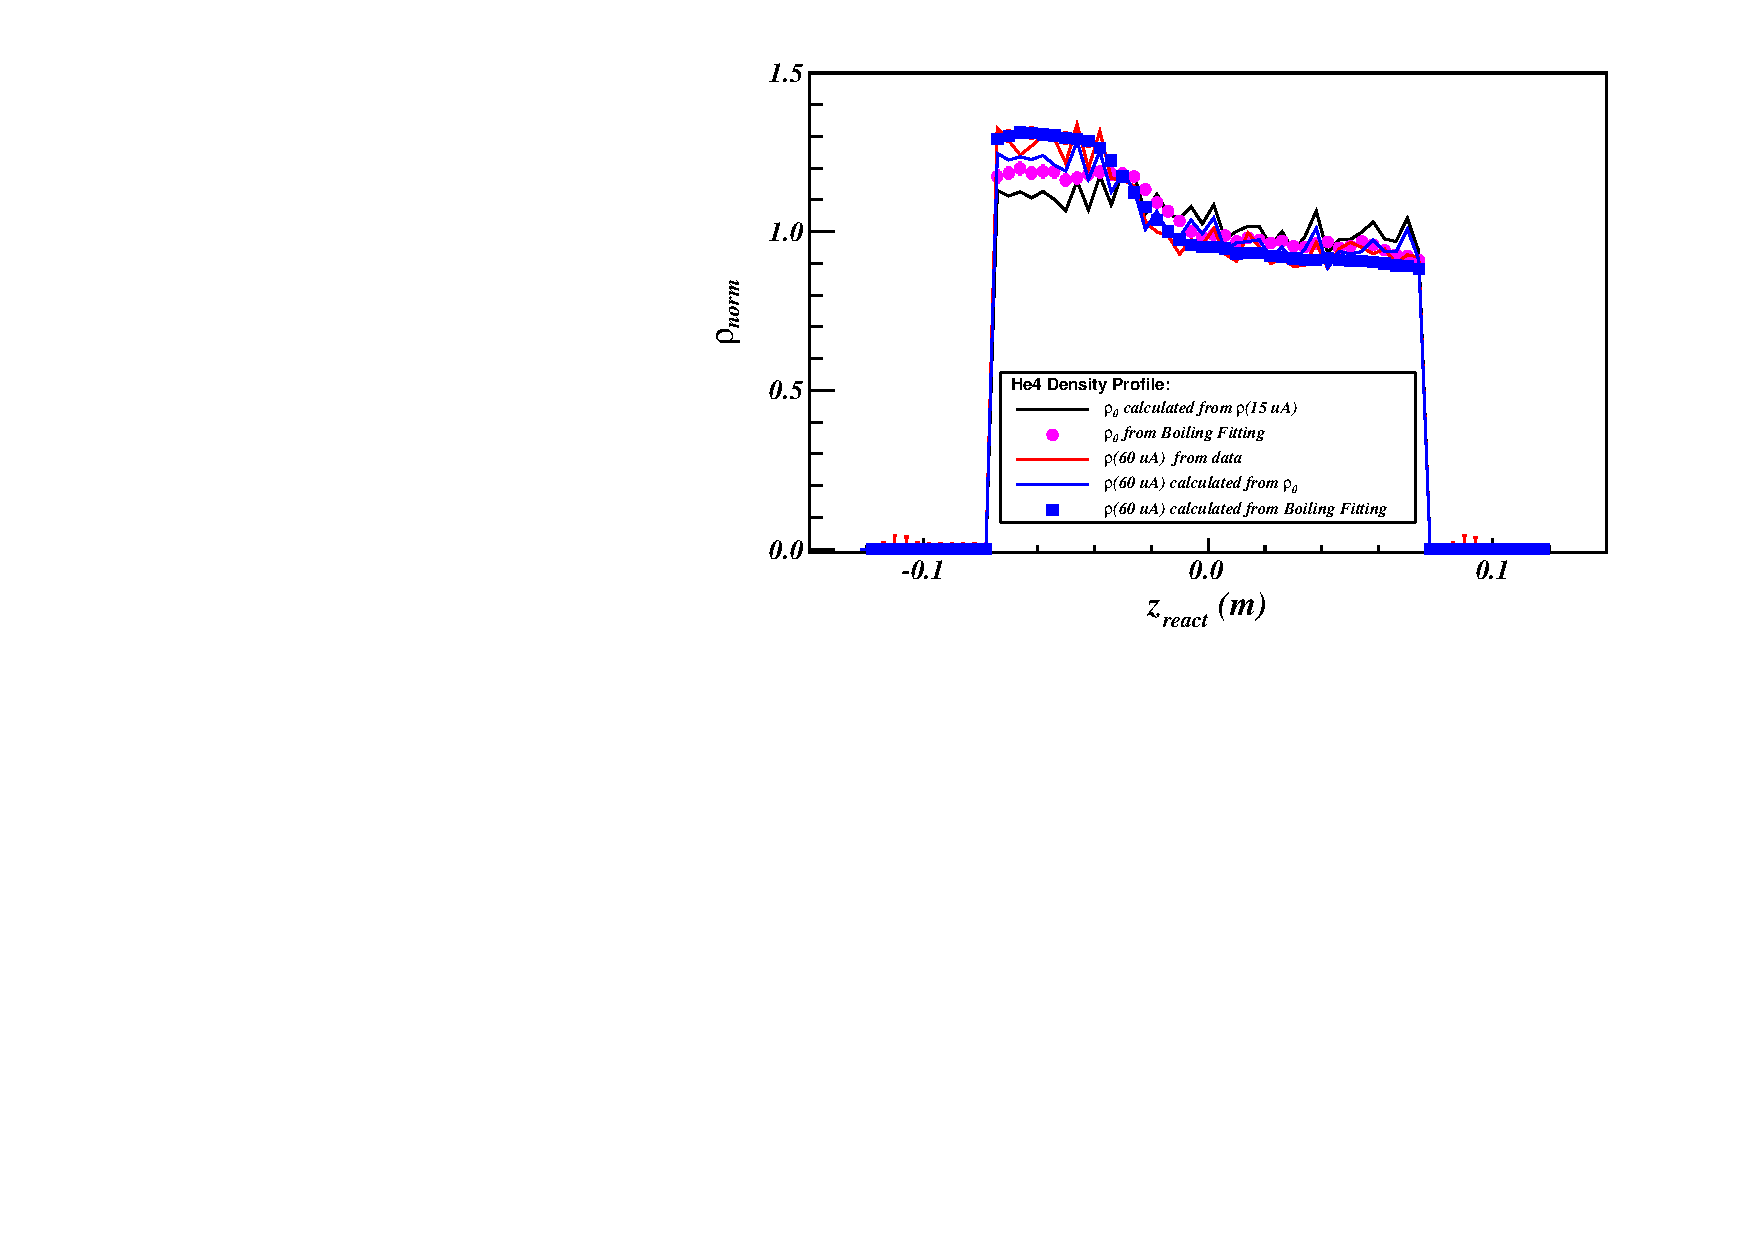
\includegraphics[type=pdf,ext=.pdf,read=.pdf,width=0.45\textwidth]{./figures/cryo/He4_Check_60} 
    }
    \hfill
    \subfloat[$\mathrm{^{4}He}$ at I=95 uA]{
      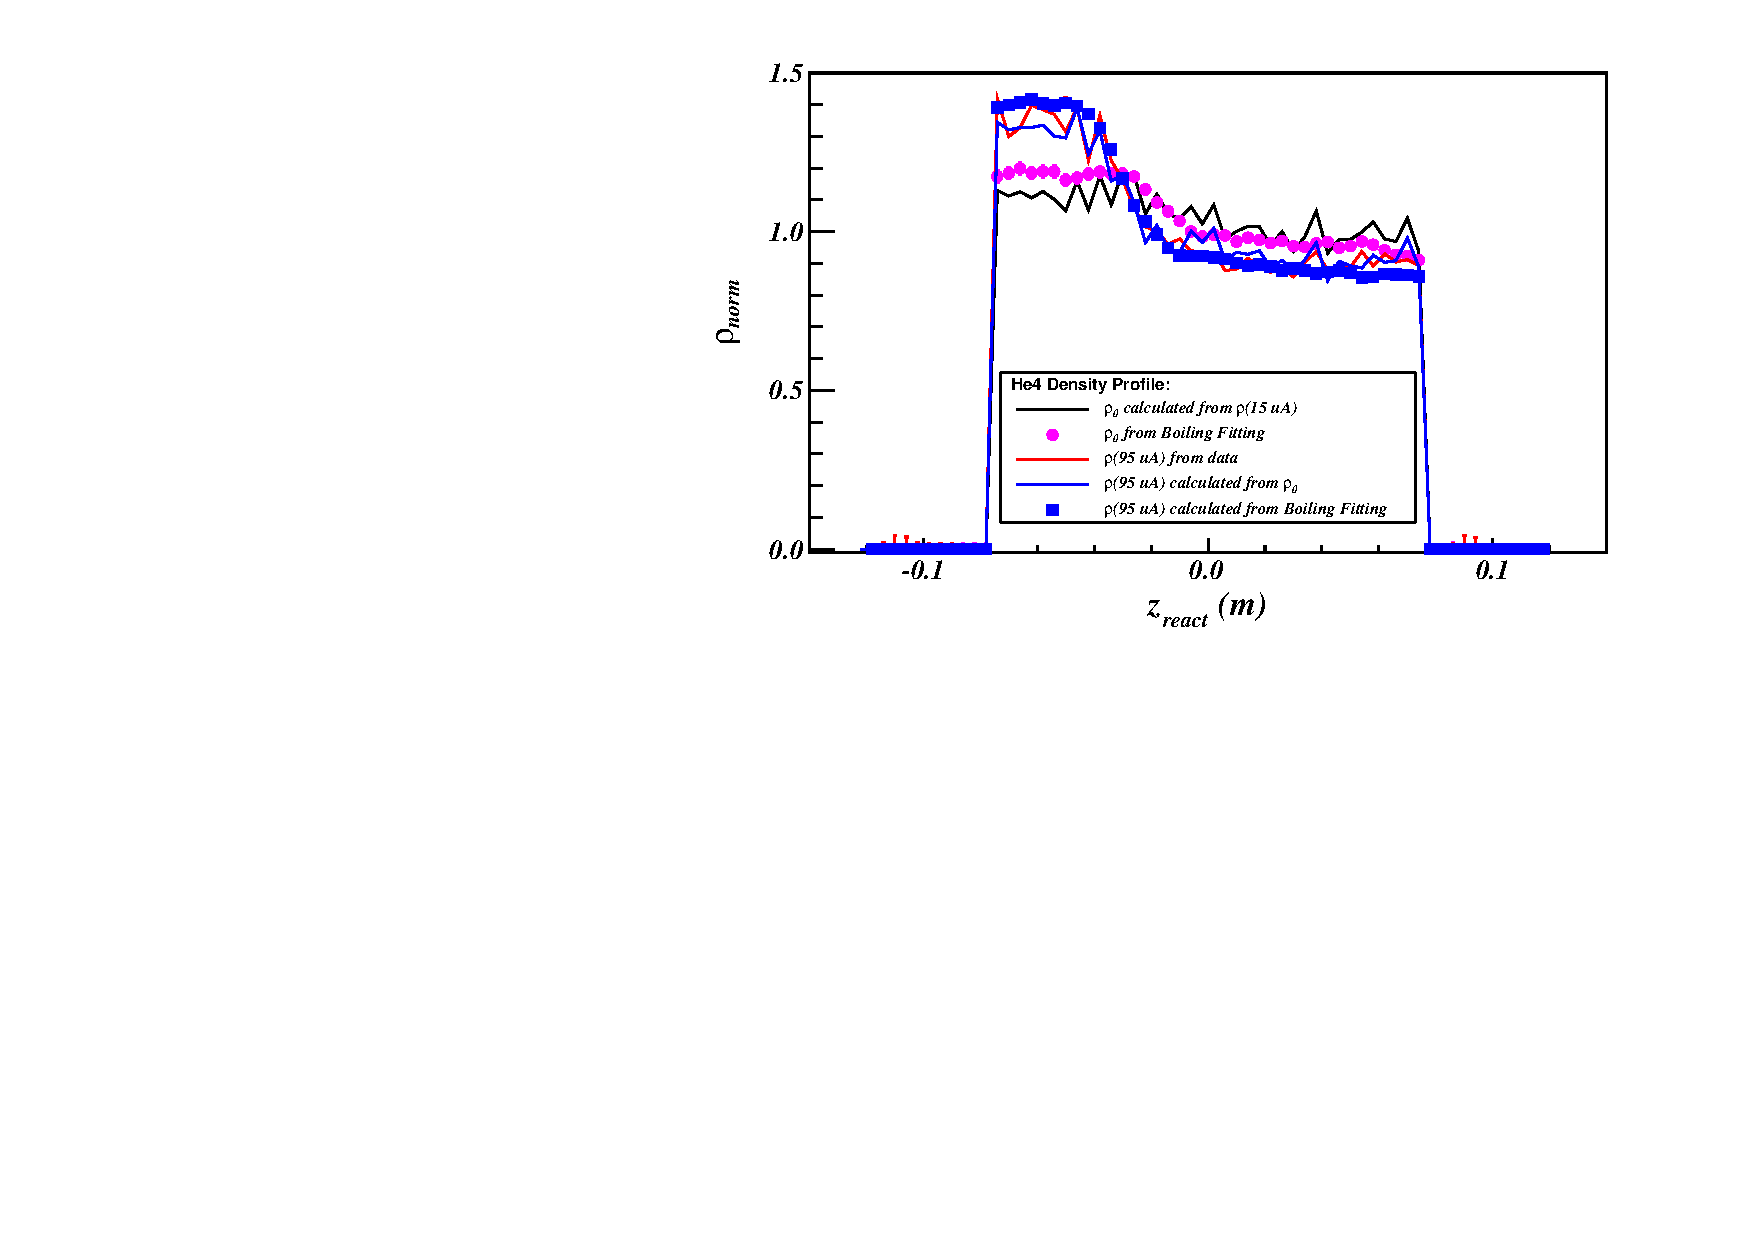
\includegraphics[type=pdf,ext=.pdf,read=.pdf,width=0.45\textwidth]{./figures/cryo/He4_Check_95} 
    }
    \caption[Cryo-targets relative density distribution]{\footnotesize{Cryo-targets relative density distribution extracted from data and corrected by the boiling factors. The density values were calculated in each $z_{react}$ bin and the peaks in these distribution were due to the statistical fluctuation. To remove the contribution of the endcaps, a cut was apply on the target length, $\mathrm{|z_{react}|\leq 7.5~cm}$}}
    \label{cryo_den_comp}
  \end{center}
\end{figure}

 Fig.~\ref{cryo_den_comp} also compares the distributions of the target density obtained from the boiling study and from the method discussed in this section. Ignoring the statistical fluctuations of the histograms, both methods give similar density profiles, and the small difference can be explained by the errors of the HRS acceptance simulation in SAMC and the cross section model in XEMC.
 
\section{Absolute Density}
 When the density distribution is uniform, the absolute density of a cryo-target can be calculated with the temperature and pressure readings from the target system with the fixed volume of the target cell. However, the calculation becomes impossible when the density is not uniform since the temperature and pressure fluctuate inside the target. While the relative density distribution has been extracted as discussed in previous section, one can obtain the absolute density distribution by calculating the density at the entrance of the target cell where the temperature and pressure were monitored.
 
  Whereas, the extracted relative density distribution at the entrance does not reflect the true density profile of the cryo-target due to the contamination of the aluminium endcaps during the boiling study, and an assumption has been made to assign the density value at the entrance to the value at $\mathrm{-10\leq z_{react} \leq -7.5~cm}$. The true value should not deviate too far away from this value since this location is very close to the entrance and the coolant flow should be able to maintain the same temperature as it at the entrance. The deviation can be corrected when comparing the experimental yield and the simulation yield, while the last one, yet, depends on the cross section model. To obtain the accurate density, one can utilize the 2N-SRC plateaus of cross section ratio of the carbon target to the cryo-targets~\cite{SLAC_Measurement_PRC.48.2451,PhysRevLett.96.082501,PhysRevLett.108.092502}, which have been well measured in previous experiments. Table~\ref{cryo_density_table} gives the densities of cryo-targets at the entrance and the yield-normalized density at $\mathrm{z_{react}=7.5~cm}$, where the values will be updated when they are further normalized by the 2N-SRC plateaus.
\begin{table}[htbp]
 \begin{tabular}{lcccccccc}
 \toprule
 Target:                        & $\mathrm{^{2}H}$  & $\mathrm{^{3}He}$-I  & $\mathrm{^{3}He}$-II & $\mathrm{^{4}He}$ \\
 \midrule
 $\rho_{entrance}~(g/cm^{3})$:   & 0.1676   & 0.0213      &  0.0296     & 0.0324 \\
 $\rho_{z_{react}=-7.5~cm}~(g/cm^{3})$:&  0.1906  & 0.0210 &  0.0292    & 0.0280 \\
 \bottomrule
 \end{tabular}
% \centering
\caption[Cryo-targets densities]{\footnotesize{Cryo-targets densities, where two values of the $\mathrm{^{3}He}$ density refer to two different run periods. The values of $\rho_{entrance}$ are calculated from the temperature and pressure reading~\cite{target_report}. The values of $\rho_{z_{react}}=-7.5~cm$ are the values of $\rho_{entrance}$ normalized by the ratio of the experimental yield and the simulation yield and will be further corrected by comparing the 2N-SRC plateaus.}}
\label{cryo_density_table}
\end{table}

\section{Radiative Correction}
  The most essential parameter during the radiative correction is the radiation length of the target. For a uniform target, the radiation length is evaluated at the center of the target. For a non-uniform target, such an approximation has to be carefully examined. 

\begin{figure}[!ht]
 \begin{center}
  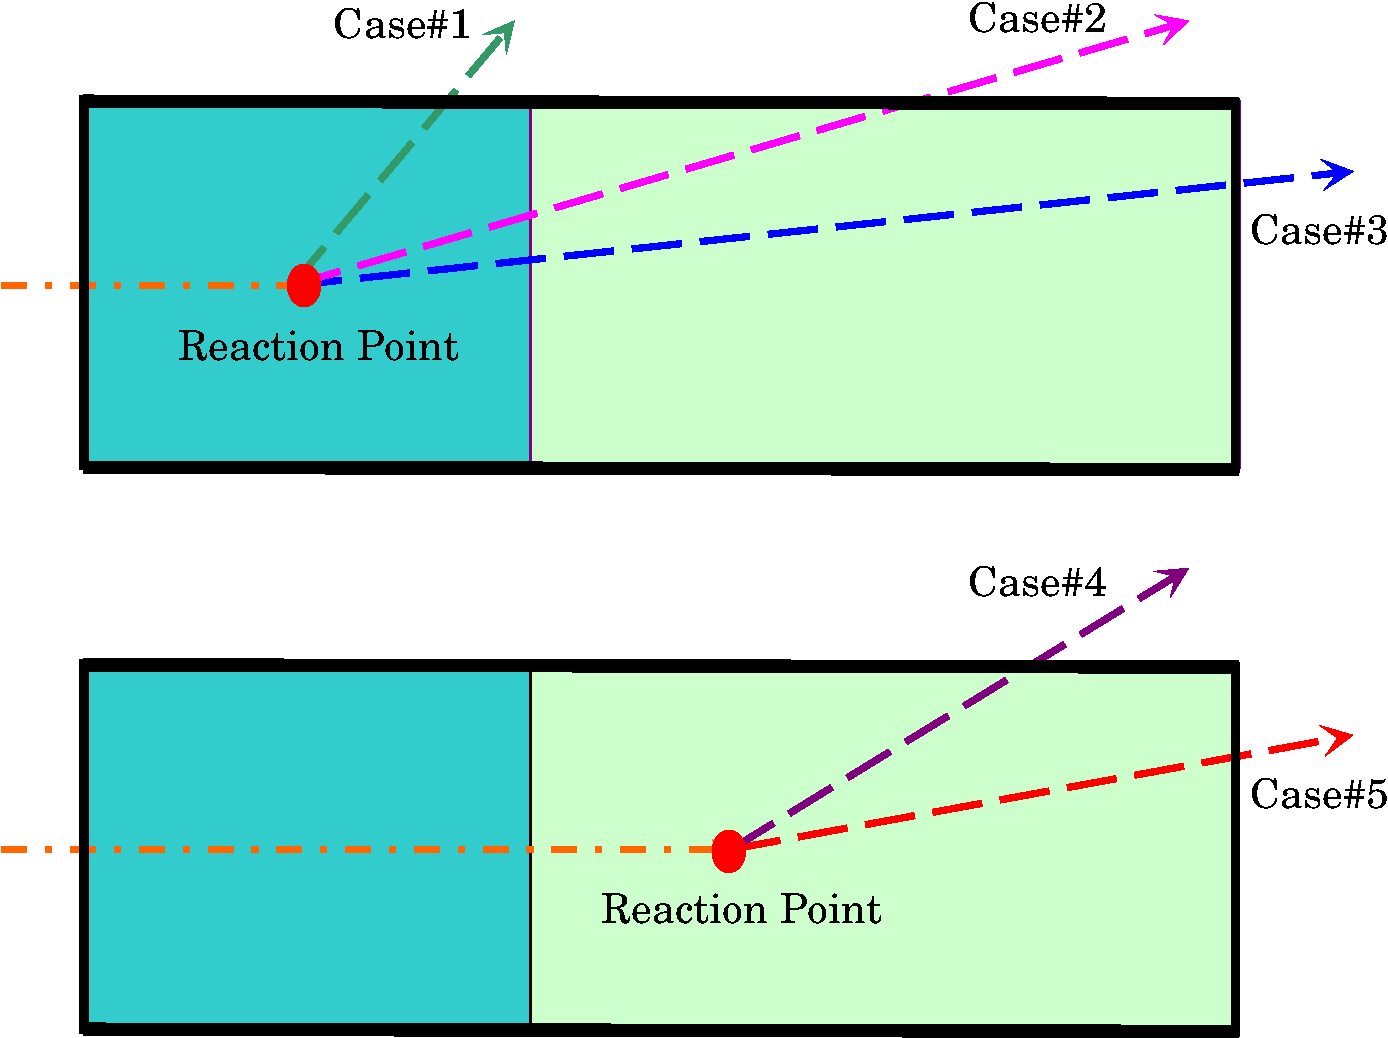
\includegraphics[angle=0,width=0.6\textwidth]{./figures/xemc/radc_cases}
  \caption[Different cases to calculate the radiation lengths]{\footnotesize{Different cases to calculate the radiation lengths, where the target has two parts with different density. The target cell's entrance, exit and wall (black lines ) also have different thickness. Depending on the reaction point in the forward scattering, there are five cases which give different radiation lengths.}}
  \label{radc_cases}
 \end{center}
\end{figure}
  In the radiative correction model in XEMC, the density distribution of a cryo-target is simplified as a step function, where the density is 30\% higher for -10~cm$\mathrm{\leq Z_{react}}\leq$-2~cm and is 20\% lower for the rest of the target. The value of radiation length in such a distribution depends on the reaction location and the scattering angle. Fig.~\ref{radc_cases} gives 5 different scattering paths which have been coded in the model. 
  
 \begin{figure}[!ht]
\begin{center}
  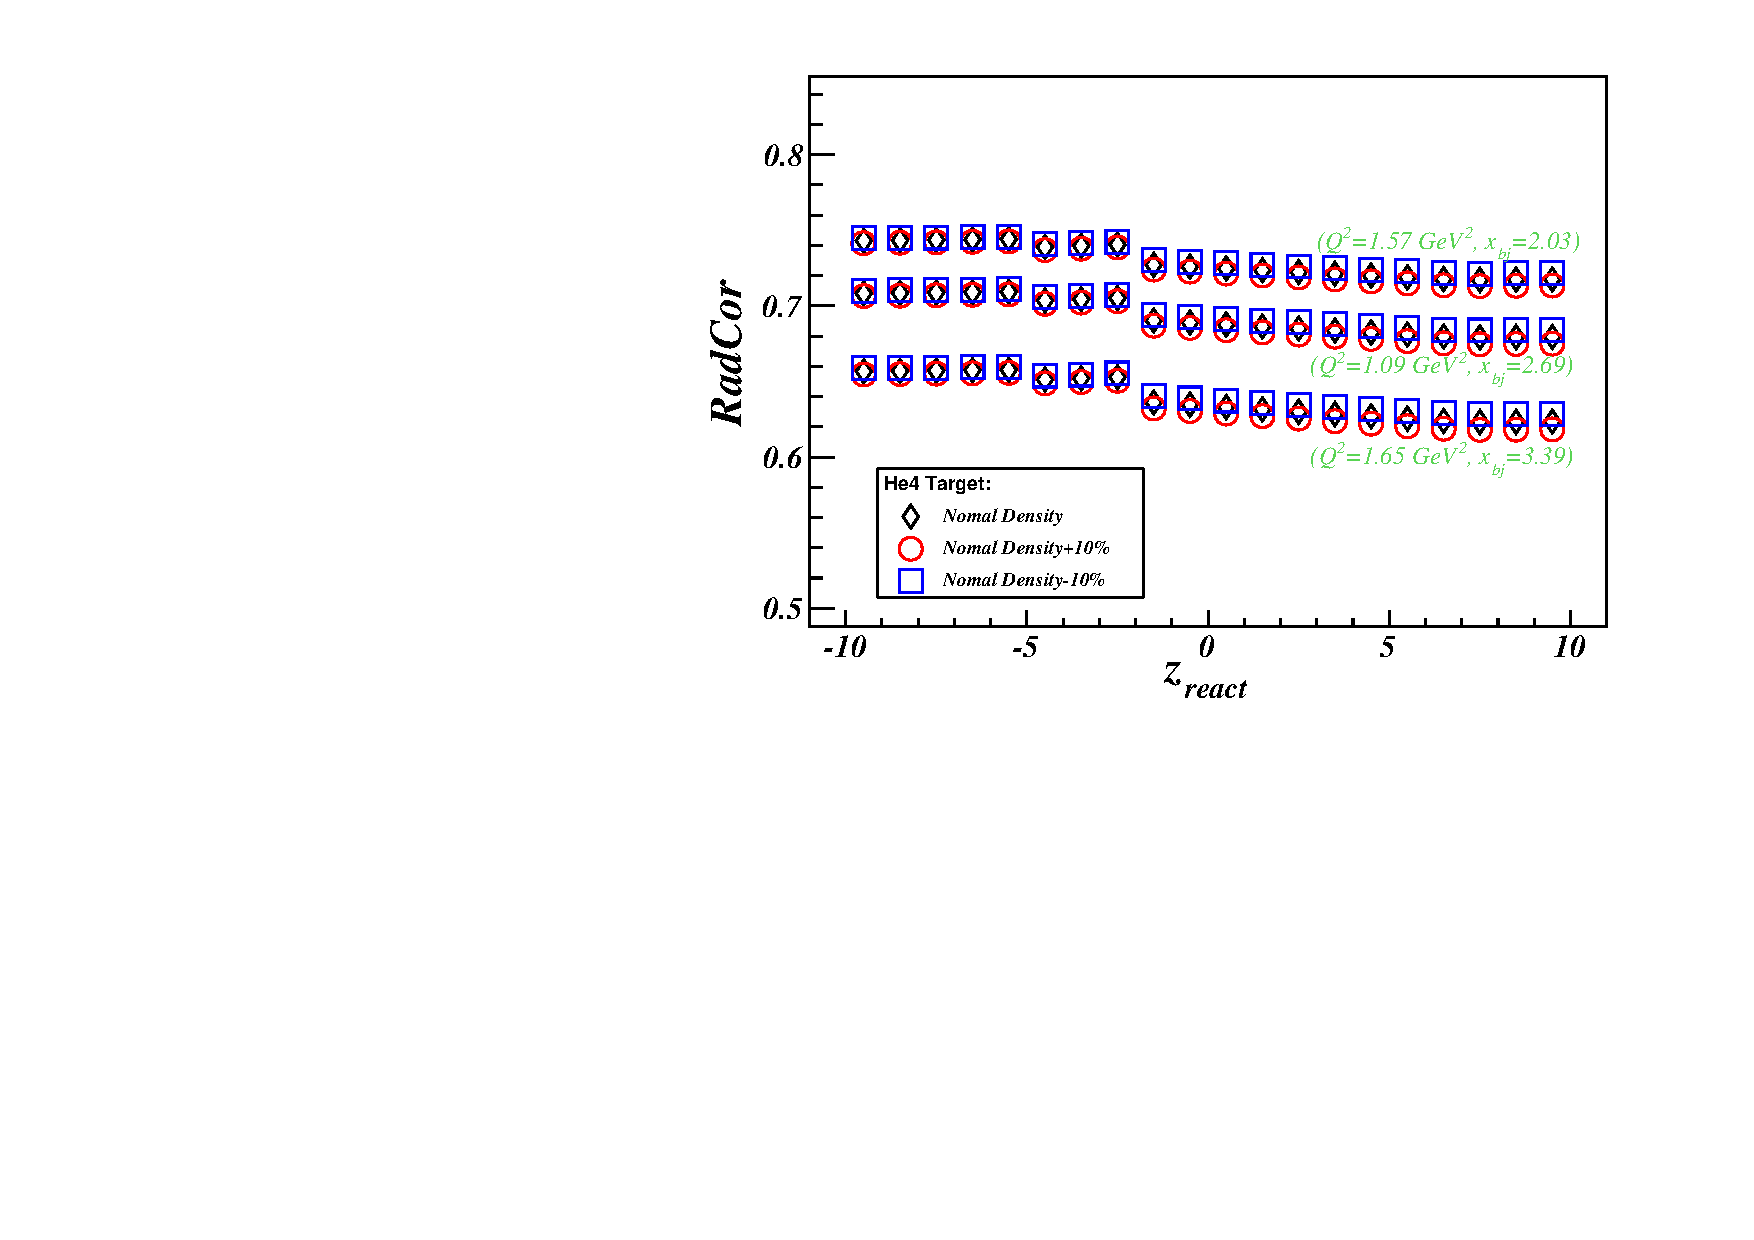
\includegraphics[angle=0,width=0.8\textwidth]{./figures/xemc/He4_RadC}
  \caption[Position dependence of radiative effect on $\mathrm{^{4}He}$]{\footnotesize{Position dependence of radiative effect on $\mathrm{^{4}He}$. With a step function as the density distribution, $\mathrm{z_{react}}$ was divided into 20 bins where in each bin radiative correction factors were calculated at three different kinematic settings. To check the variation of the absolute density, the radiative effect was calculated in each $\mathrm{z_{react}}$ bin by changing the density by $\mathrm{\pm 10}$\%. The radiative effect clearly depends on the reaction location but has small dependence on the absolute density.}}
  \label{he4_rad_check}
 \end{center}
\end{figure}
  To study the position dependence of the radiative effect, the target was divided into 20 bins along the $\mathrm{z_{react}}$ distribution where the radiative correction factor (Eq.~\eqref{eq_radc_fact}) was calculated in each bin. Fig.~\ref{he4_rad_check} shows the distribution of the radiative correction factor as a function of $\mathrm{z_{react}}$. The downstream part of the target has stronger radiative effect since the incoming electron loses more energy while passing through the upstream part which has higher density. Overall, the variation of the radiative correction factors along the target length is less than 2\%. The distributions at different kinematic settings were also studied by changing the value of $E'$ by $\mathrm{\pm}$ 3\%. The results give the similar distribution which indicates that the $\mathrm{z_{react}}$-dependence of the radiative correction factors does not change much within one kinematics.
  
   The absolute target density varies with the beam current. Even though the beam current was set to a constant value for each target, it still had fluctuations depending on the stability of the beam. As discussed in the previous section, the absolute density for cryo-targets will be further normalized by the 2N-SRC ratio. In Fig.~\ref{he4_rad_check}, the radiative effect at different target densities was also examined and the results showed very small deviation when changing the density by  $\mathrm{\pm}$ 10\%.
   
% As discussed in Section 5.7, the radiated cross section was not calculated event-by-event during the cross section extract. Instead, a cross section table was generated by dividing the entire kinematic space into grids, and one looked for the cross section value from the table for each event. This method can dramatically increase the speed of calculation but one has to evaluate the radiative correct at the center of the target with the uniform density equal to the average value of the whole target. For uniform targets this method is approximately accurate. However, when the target density is non-uniform, more events come from the dense part of the target which has stronger radiative effect. 
    
% The radiative correction factor at a position on $\mathrm{z_{react}}$ was weighted by the relative density in this location, and the average value of all these factors was compared with the value calculated at the center of the target after assuming the target to be uniform and its density equal to the average density. The study showed a X\% difference between this two values.
\chapter{Cross Section Results}

%\section{Yields}

\section{Cross Sectionss}
The measured born cross sections for $\mathrm{^{2}H}$, $\mathrm{^{3}He}$,$\mathrm{^{4}He}$,$\mathrm{^{12}C}$,$\mathrm{^{40}Ca}$,and $\mathrm{^{48}Ca}$ are shown in Fig.~\ref{xs_born_h2} through Fig.~\ref{xs_born_ca48}, respectively. Note that only the systematic errors from the detectors and the statistical errors are included. There are several other sources of systematic errors needed to be evaluated, e.g. the cryogenic target densities, acceptance correction, bin-centering correction and radiative corrections. etc..

 The detailed kinematic settings of two HRSs and list of targets measured are given in Table~\ref{kine_table_left} and Table~\ref{kine_table_right}. For each setting, if data is available from both arms, the cross section values are given as the average of individual cross sections extracted from these arms. 
\begin{table}[!ht]
  \centering
  \begin{tabular}{|c|c|c|c|c|}
    \hline
    Name      &  $\theta_{0} (^{o})$    & $P_{0}~(GeV/c)$ & $Q^{2}~(GeV^{2})$ &  Target \\
    \hline 
     Kin3.1   &21     & 2.905           & 1.295        & $^{2}H$,$^{3}He$, $^{4}He$,$^{12}C$,$^{40}Ca$,$^{48}Ca$ \\
    \hline                      
     Kin3.2   &21     & 3.055           & 1.362        &         $^{3}He$, $^{4}He$,$^{12}C$,                    \\
     \hline 
     Kin4.1   &23     & 2.855           & 1.523        &         $^{3}He$,          $^{12}C$,$^{40}Ca$,$^{48}Ca$ \\
      \hline 
     Kin4.2   &23     & 3.035           & 1.619        &         $^{3}He$, $^{4}He$,$^{12}C$,$^{40}Ca$,$^{48}Ca$ \\
     \hline 
     Kin5.0   &25     & 2.505           & 1.575        &         $^{3}He$, $^{4}He$,$^{12}C$,$^{40}Ca$,$^{48}Ca$ \\
     \hline 
     Kin5.05  &25     & 2.650           & 1.667        &         $^{3}He$,         $^{12}C$,$^{40}Ca$,$^{48}Ca$ \\
     \hline    
     Kin5.1   &25     & 2.795           & 1.758        &$^{2}H$, $^{3}He$, $^{4}He$,$^{12}C$,$^{40}Ca$,$^{48}Ca$ \\
     \hline    
     Kin5.2   &25     & 2.995           & 1.883        &$^{2}H$, $^{3}He$, $^{4}He$,$^{12}C$                     \\
    \hline 
     Kin6.5   &28     & 2.845           & 2.235        &          $^{3}He$,        $^{12}C$,                    \\
    \hline 
   \end{tabular}
  \caption[List of kinematic settings and target measured on HRS-L]{List of kinematic settings and targets measured on HRS-L}
  \label{kine_table_left}	
\end{table}
\begin{table}[!ht]
  \centering
  \begin{tabular}{|c|c|c|c|c|}
    \hline
    Name      &  $\theta_{0} (^{o})$    & $P_{0}~(GeV/c)$ & $Q^{2}~(GeV^{2})$ &  Target \\
    \hline 
     Kin3.1   &21     & 2.905           & 1.295   & $^{2}H$,          $^{4}He$,$^{12}C$,$^{40}Ca$,$^{48}Ca$ \\
    \hline                      
     Kin3.2   &21     & 3.055           & 1.362   &          $^{3}He$,$^{4}He$,$^{12}C$,$^{40}Ca$,$^{48}Ca$ \\
     \hline 
     Kin4.1   &23     & 2.855           & 1.523   &          $^{3}He$,         $^{12}C$,$^{40}Ca$,$^{48}Ca$ \\
      \hline 
     Kin4.2   &23     & 3.035           & 1.619   &          $^{3}He$,$^{4}He$,$^{12}C$,$^{40}Ca$,$^{48}Ca$ \\
     \hline 
     Kin5.0   &25     & 2.505           & 1.575   &          $^{3}He$,$^{4}He$,$^{12}C$,$^{40}Ca$,$^{48}Ca$ \\
     \hline 
     Kin5.05  &25     & 2.650           & 1.667   &                                                         \\
     \hline    
     Kin5.1   &25     & 2.795           & 1.758   & $^{2}H$, $^{3}He$,$^{4}He$,$^{12}C$,$^{40}Ca$,$^{48}Ca$ \\
     \hline    
     Kin5.2   &25     & 2.995           & 1.883   & $^{2}H$, $^{3}He$,$^{4}He$,$^{12}C$                     \\
    \hline 
     Kin6.5   &28                       & 2.845           & 2.235   &          $^{3}He$,        $^{12}C$,                    \\    
    \hline 
   \end{tabular}
  \caption[List of kinematic settings and target measured on HRS-R]{List of kinematic settings and target measured on HRS-R}
  \label{kine_table_right}	
\end{table}
  
 Fig.~\ref{xs_born_h2} shows the cross section of $\mathrm{^{2}H}$, where the Quasielastic (QE) peak can be clearly identified at $x_{bj}=1$ due to the relatively small Fermi motion of nucleons in the target. The results show good agreement with the calculation from XEMC model. $\mathrm{^{4}He}$ and $\mathrm{^{12}C}$ agree nicely with the model prediction (Fig.~\ref{xs_born_he4} and Fig.~\ref{xs_born_c12}). For $\mathrm{^{3}He}$ target, additional work is required on the XEMC model to correct the rapidly decreasing of cross section values when $x_{bj}\rightarrow 3$. Cross sections of $\mathrm{^{40}Ca}$ and $\mathrm{^{48}Ca}$ at high $\mathrm{Q^{2}}$ ($\mathrm{>1~GeV^{2}}$) are only available from this experiment and more iterations of the cross section models are necessary until the model and the data have solid agreement.
 
\begin{figure}[!ht]
  \begin{center}
    \subfloat[$\sigma^{^{2}H}_{born}$ .vs. $\nu$]{
      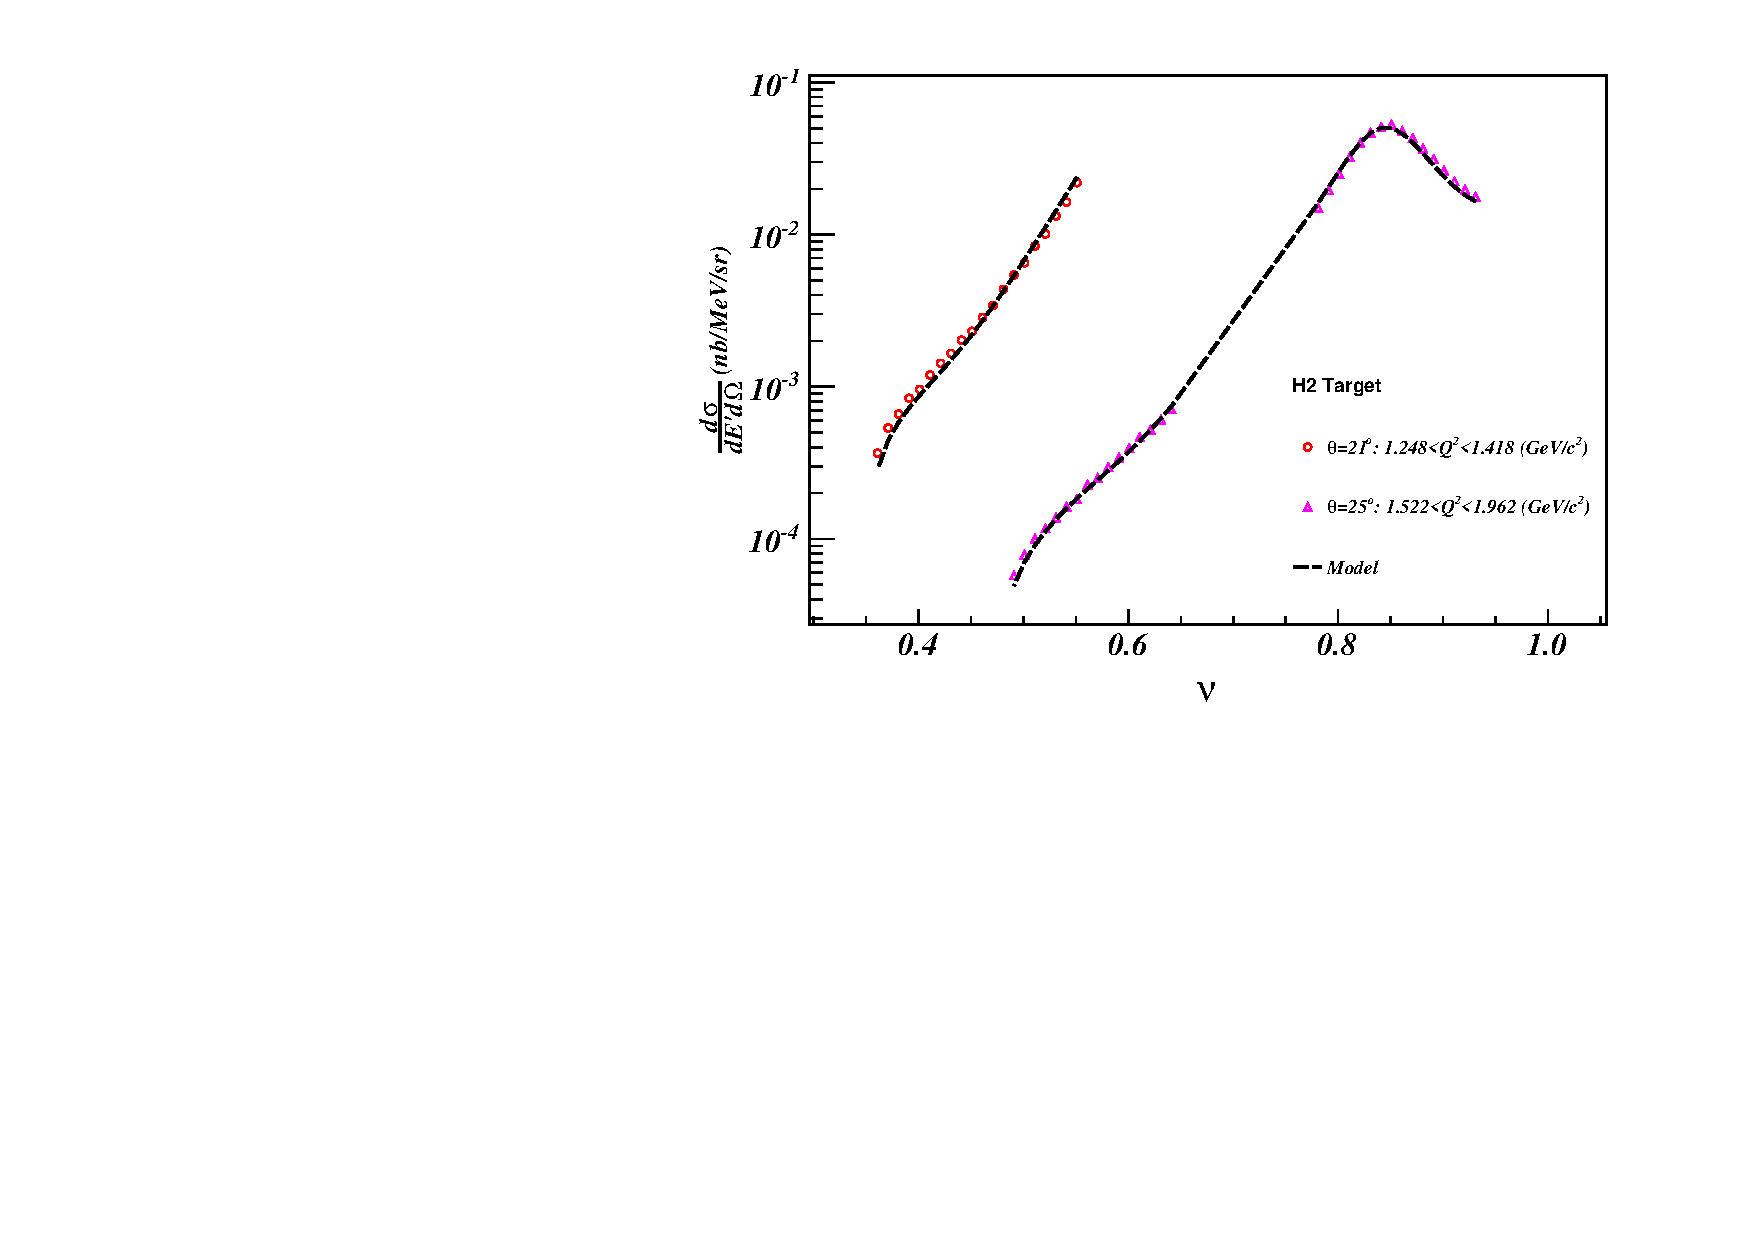
\includegraphics[type=pdf,ext=.pdf,read=.pdf,width=0.90\textwidth]{./figures/xs/H2_XS_All}
    }
    \\
    \subfloat[$\sigma^{^{2}H}_{born}$ .vs. $x_{bj}$]{
      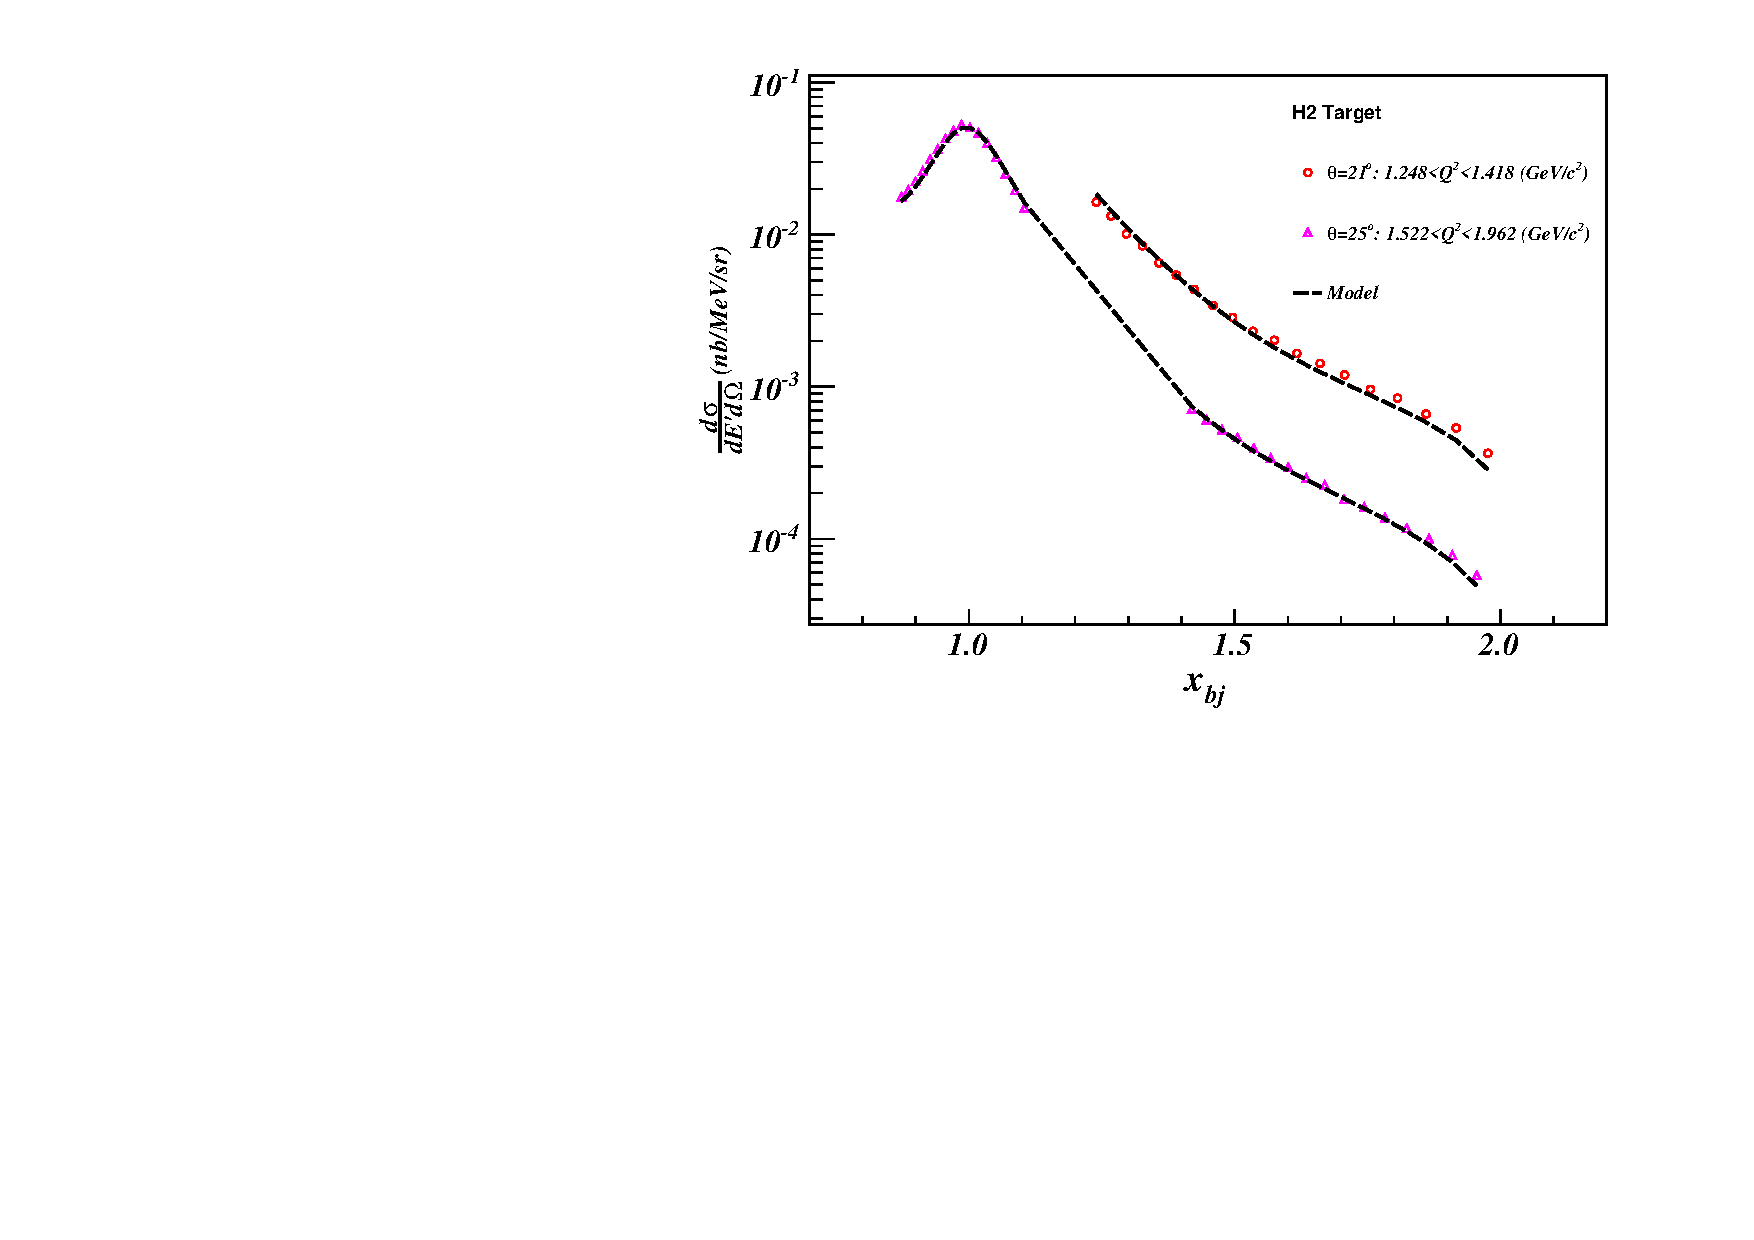
\includegraphics[type=pdf,ext=.pdf,read=.pdf,width=0.90\textwidth]{./figures/xs/H2_XS_All_xbj}
    }
    \caption[$\mathrm{^{2}H}$ preliminary born cross sections]{\footnotesize{$\mathrm{^{2}H}$ preliminary born cross sections, where dots are from experimental results and lines are calculated from XEMC model}}
    \label{xs_born_h2}
  \end{center}
\end{figure}
\begin{figure}[!ht]
  \begin{center}
    \subfloat[$\sigma^{^{3}He}_{born}$ .vs. $\nu$]{
      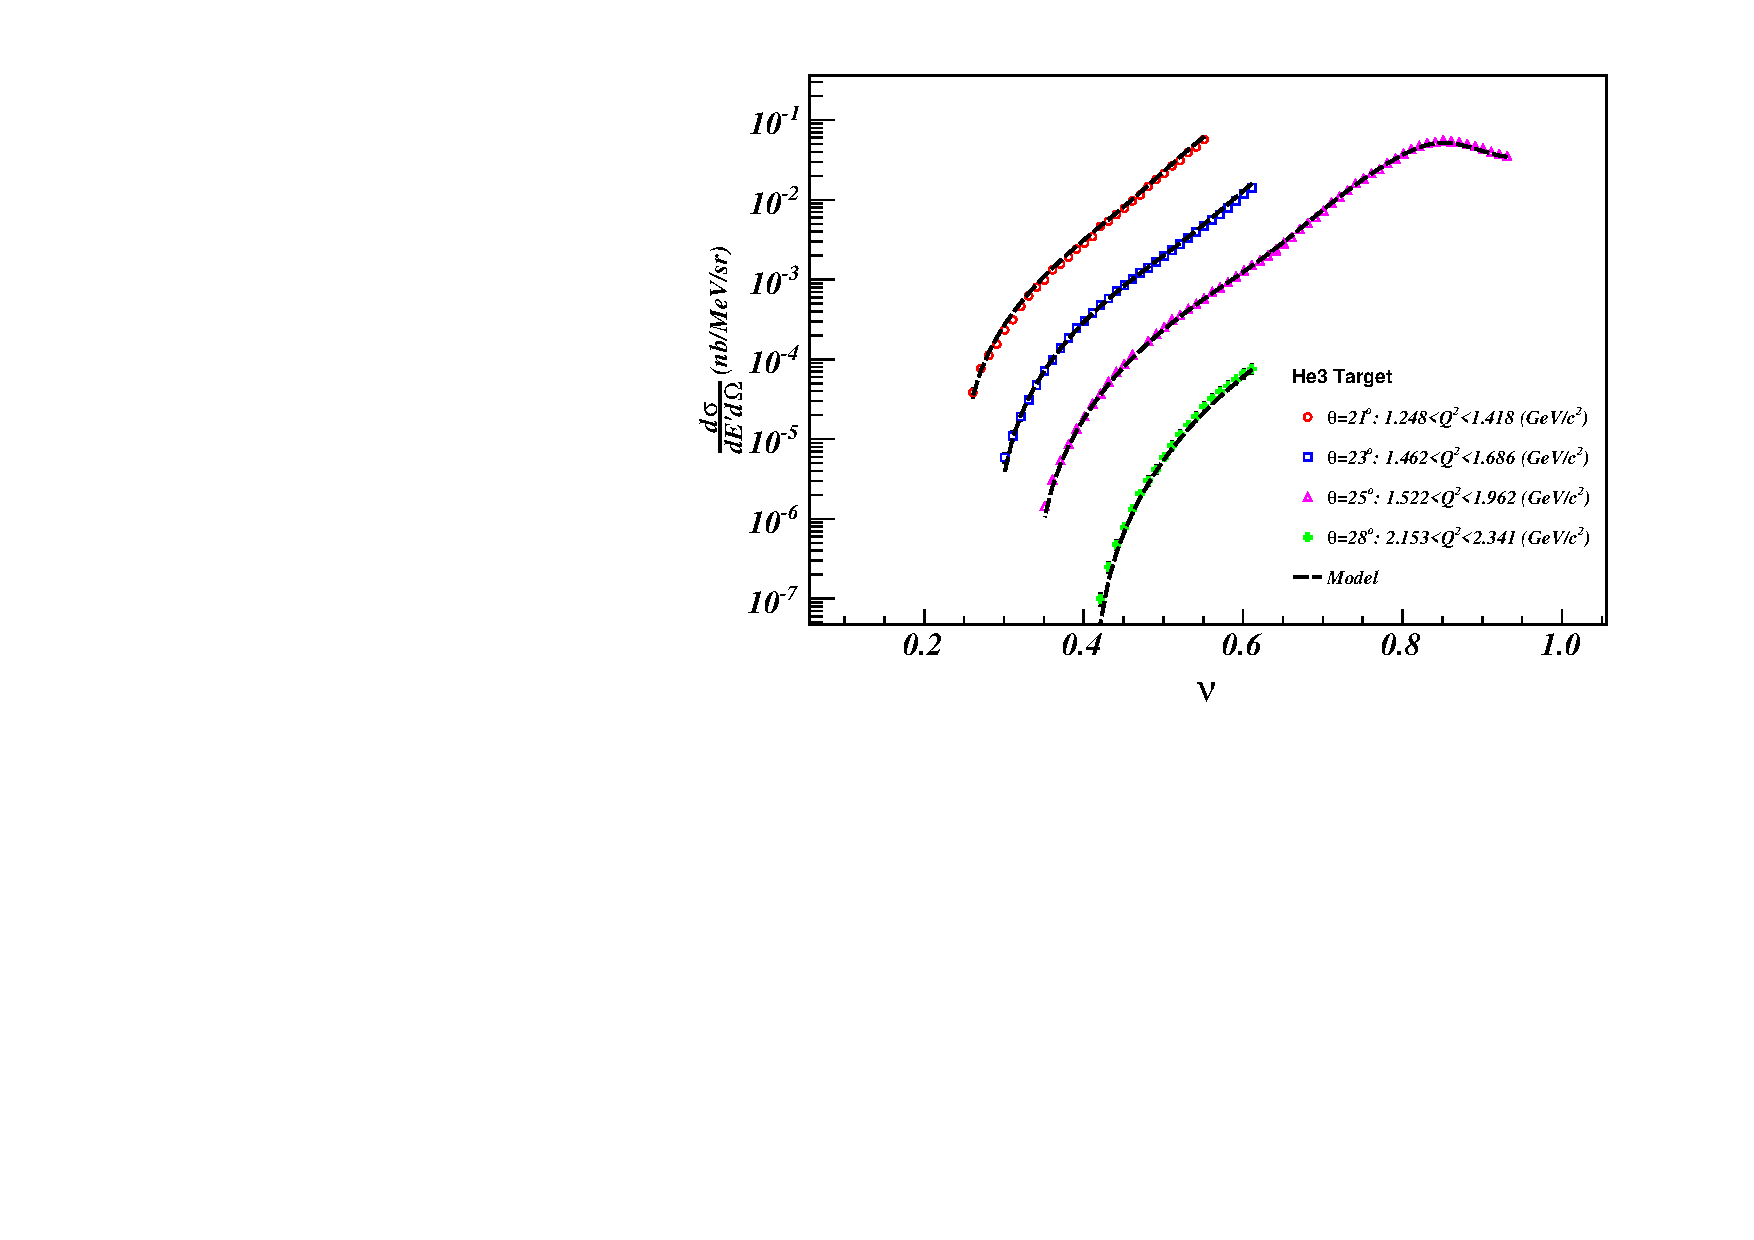
\includegraphics[type=pdf,ext=.pdf,read=.pdf,width=0.90\textwidth]{./figures/xs/He3_XS_All}
    }
    \\
    \subfloat[$\sigma^{^{3}He}_{born}$ .vs. $x_{bj}$]{
      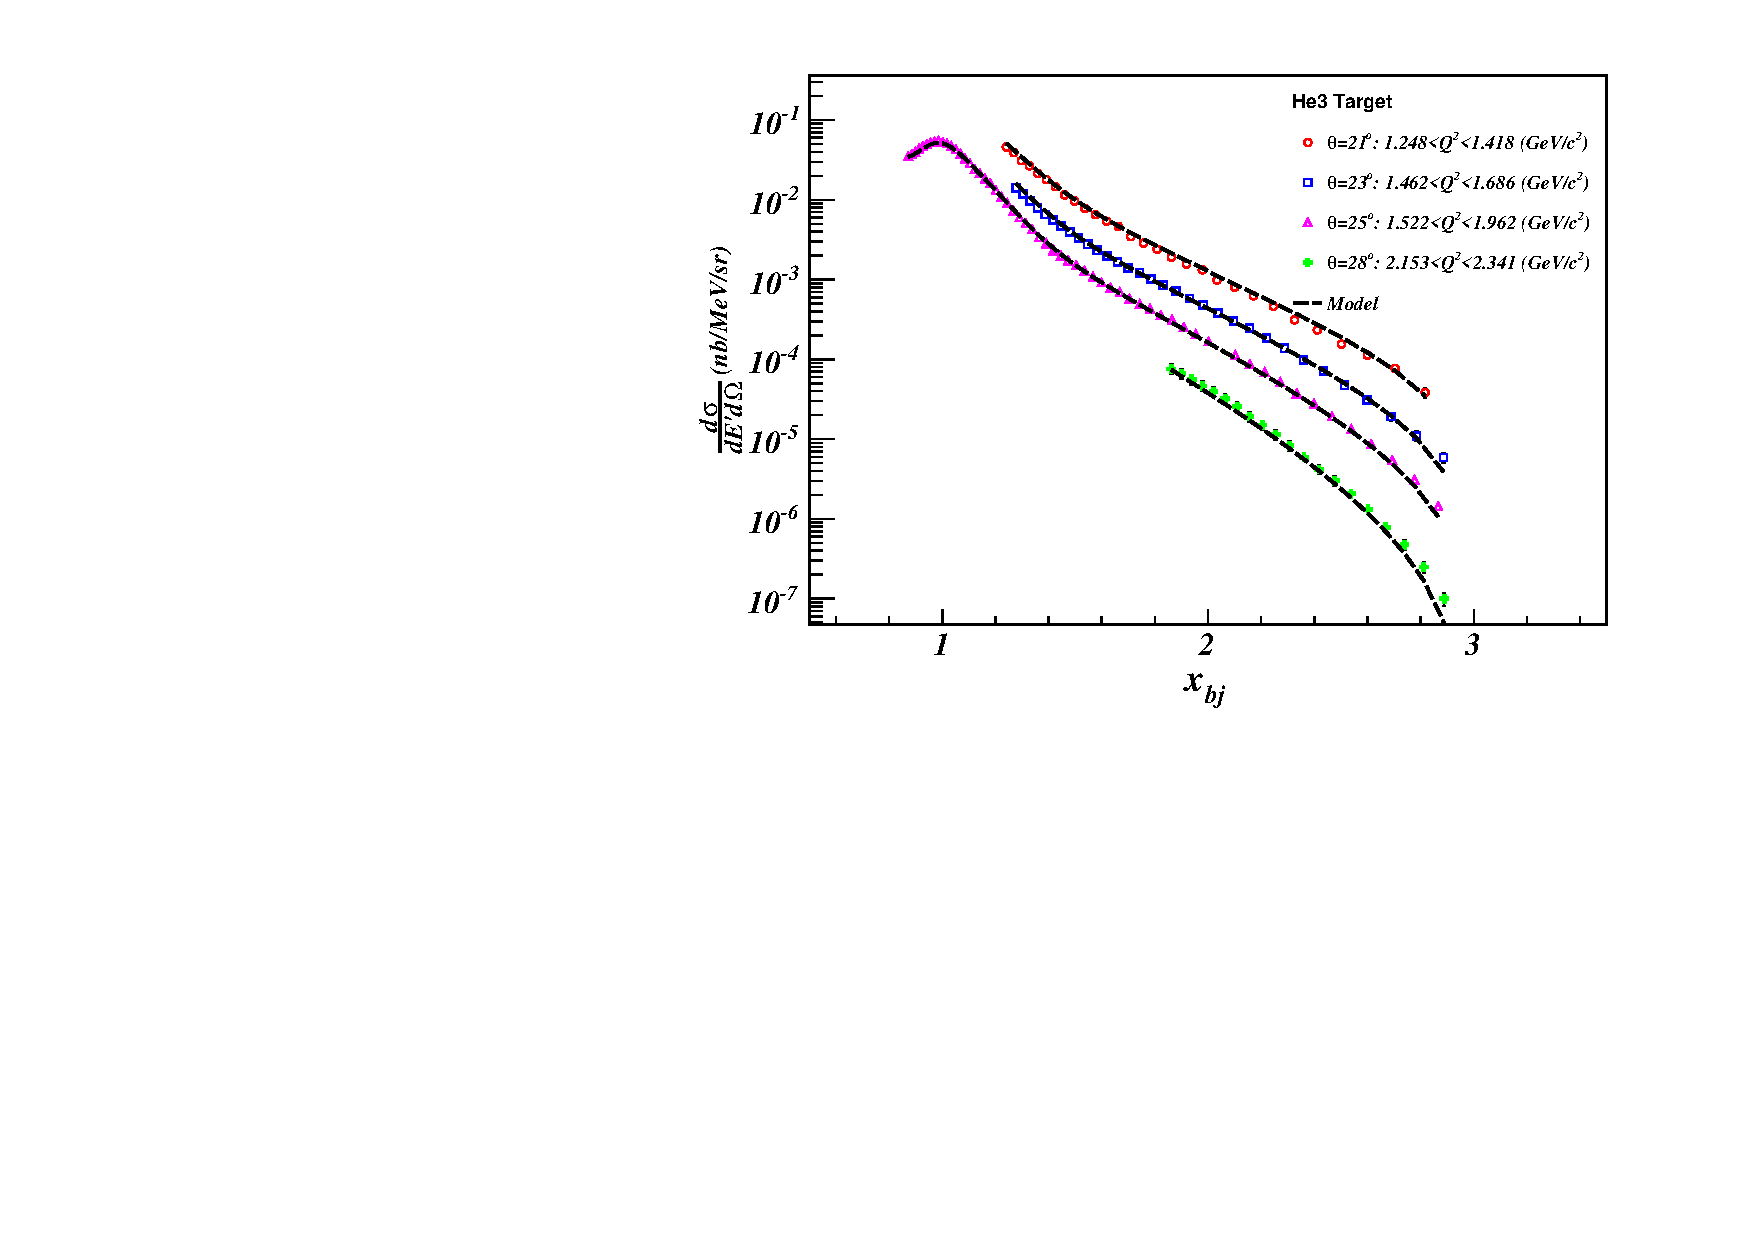
\includegraphics[type=pdf,ext=.pdf,read=.pdf,width=0.90\textwidth]{./figures/xs/He3_XS_All_xbj}
    }
    \caption[$\mathrm{^{3}He}$ preliminary born cross sections]{\footnotesize{$\mathrm{^{3}He}$ preliminary born cross sections, where dots are from experimental results and lines are calculated from XEMC model}}
    \label{xs_born_he3}
  \end{center}
\end{figure}
  \begin{figure}[!ht]
  \begin{center}
    \subfloat[$\sigma^{^{4}He}_{born}$ .vs. $\nu$]{
      \includegraphics[type=pdf,ext=.pdf,read=.pdf,width=0.90\textwidth]{./figures/xs/He4_XS_All}
    }
    \\
    \subfloat[$\sigma^{^{4}He}_{born}$ .vs. $x_{bj}$]{
      \includegraphics[type=pdf,ext=.pdf,read=.pdf,width=0.90\textwidth]{./figures/xs/He4_XS_All_xbj}
    }
    \caption[$\mathrm{^{4}He}$ preliminary born cross sections]{\footnotesize{$\mathrm{^{4}He}$ preliminary born cross sections, where dots are from experimental results and lines are calculated from XEMC model}}
    \label{xs_born_he4}
  \end{center}
\end{figure}

  \begin{figure}[!ht]
  \begin{center}
    \subfloat[$\sigma^{^{12}C}_{born}$ .vs. $\nu$]{
      \includegraphics[type=pdf,ext=.pdf,read=.pdf,width=0.90\textwidth]{./figures/xs/C12_XS_All}
    }
    \\
    \subfloat[$\sigma^{^{12}C}_{born}$ .vs. $x_{bj}$]{
      \includegraphics[type=pdf,ext=.pdf,read=.pdf,width=0.90\textwidth]{./figures/xs/C12_XS_All_xbj}
    }
    \caption[$\mathrm{^{12}C}$ preliminary born cross sections]{\footnotesize{$\mathrm{^{12}C}$ preliminary born cross sections, where dots are from experimental results and lines are calculated from XEMC model}}
    \label{xs_born_c12}
  \end{center}
\end{figure}

  \begin{figure}[!ht]
  \begin{center}
    \subfloat[$\sigma^{^{40}Ca}_{born}$ .vs. $\nu$]{
      \includegraphics[type=pdf,ext=.pdf,read=.pdf,width=0.90\textwidth]{./figures/xs/Ca40_XS_All}
    }
    \\
    \subfloat[$\sigma^{^{40}Ca}_{born}$ .vs. $x_{bj}$]{
      \includegraphics[type=pdf,ext=.pdf,read=.pdf,width=0.90\textwidth]{./figures/xs/Ca40_XS_All_xbj}
    }
    \caption[$\mathrm{^{40}Ca}$ preliminary born cross sections]{\footnotesize{$\mathrm{^{40}Ca}$ preliminary born cross sections, where dots are from experimental results and lines are calculated from XEMC model}}
    \label{xs_born_ca40}
  \end{center}
  \end{figure}
  
  \begin{figure}[!ht]
  \begin{center}
    \subfloat[$\sigma^{^{48}Ca}_{born}$ .vs. $\nu$]{
      \includegraphics[type=pdf,ext=.pdf,read=.pdf,width=0.90\textwidth]{./figures/xs/Ca48_XS_All}
    }
    \\
    \subfloat[$\sigma^{^{48}Ca}_{born}$ .vs. $x_{bj}$]{
      \includegraphics[type=pdf,ext=.pdf,read=.pdf,width=0.90\textwidth]{./figures/xs/Ca48_XS_All_xbj}
    }
    \caption[$\mathrm{^{48}Ca}$ preliminary born cross sections]{\footnotesize{$\mathrm{^{48}Ca}$ preliminary born cross sections, where dots are from experimental results and lines are calculated from XEMC model}}
    \label{xs_born_ca48}
  \end{center}
\end{figure}
%\section{Errors}
%The error bars shown here are calculated based on the discussion given in Chapter 5. 

%\begin{table}[!ht]
%  \centering
%  \begin{tabular}{|c|c|c|c|c|}
%    \hline
%    Source                   &  Scale   & Relative &  $\mathrm{\Delta\sigma/\sigma}$ & Comment\\
%    \hline\hline 
%    Trigger Efficiency       &  -       & 0.1\%    &                                 &        \\
%    Live-time                &  0.1\%   &  -       &                                 &        \\
%    VDC One-Track Efficiency &  0.4\%   & 0.3\%    &                                 &        \\
%    PID Efficiency           &  0.05\%  & 0.3\%    &                                 &        \\
%    \hline
%    Target Thickness         &0.5-2.4\% & -        &                                 &        \\
%    Beam Charge              &  0.4\%   & 0.3\%    &                                 &        \\
%    Beam Energy              & 0.05\%   & 0.02\%   &                                 &        \\
%    \hline
%    HRS-L Momentum           & 0.05\%   & 0.01\%   &                                 &        \\
%    HRS-L Angle              & 0.05\%   & 0.01\%   &                                 &        \\
%    HRS-R Momentum           & 0.05\%   & 0.01\%   &                                 &        \\
%    HRS-R Angle              & 0.05\%   & 0.01\%   &                                 &        \\
%    \hline    
%    Acceptance Correction    & 1\%      & 1\%      &                                 &        \\
%    Bin-Centering Correction & -        & 0.5\%    &                                 &        \\
%    Radiative Correction     & 1\%      & 1\%      &                                 &        \\
%    Coulomb Correction       & -        & 0-2\%    &                                 &        \\
%    \hline
%    Cryo-Target Boiling      &0.45\%    & 0.2\%    &                                 &        \\
%    Al End-Cups Subtraction  &$<$0.6\%  &0$\sim$1.8\% &                             &        \\
%    \hline
%   \end{tabular}
%  \caption[List of systematic errors]{List of systematic errors}
%  \label{stat_err_table}	
%\end{table}





%%%%%%%%%%%%% BIBLIOGRAPHY %%%%%%%%%%%%%%%%%%%%%%%%%%
\renewcommand{\baselinestretch}{1}\normalsize
\bibliographystyle{h-physrev3.bst}
%\bibliographystyle{nature}
\bibliography{xgt2}


\end{document}
